\documentclass[a4paper,11pt,oneside,openright]{report}
\usepackage{listings}
% Ams
\usepackage{xcolor}
\usepackage{graphicx}
\usepackage{uarial}
\renewcommand{\familydefault}{\sfdefault}
\usepackage[labelfont=bf,labelsep=period,justification=raggedright,font={sf,bf,small}]{caption}
%\usepackage[scaled]{helvet}  % Χρήση Helvetica αντί για Arial
%\renewcommand{\familydefault}{\sfdefault}  % Ορίζει προεπιλεγμένη sans-serif γραμματοσειρά
\usepackage{caption}
\captionsetup{font={sf,bf,small}, labelfont={bf}, justification=raggedright, singlelinecheck=false}    % Arial Bold 9pt, αριστερή στοίχιση
\usepackage{amsmath, amssymb}
\usepackage{placeins}
\usepackage{textcomp}
% Greek Language
\usepackage[utf8]{inputenc}
\usepackage[T1]{fontenc}
\usepackage[english,greek]{babel}
\usepackage[T1]{fontenc}
\newcommand{\en}{\foreignlanguage{english}}
\newcommand{\el}{\foreignlanguage{greek}}
\usepackage[autostyle=true]{csquotes}
\usepackage{kerkis}
\usepackage{float}
\usepackage{alphabeta}  
% Titlepage table
\usepackage{tabularx}

% Geometry
\usepackage[twoside,top=2.5cm,bottom=2.5cm,bindingoffset=1.5cm]{geometry}

% Fixes list of figures spacing
\usepackage{tocloft}
\setlength{\cftfignumwidth}{3em}
\renewcommand{\cfttoctitlefont}{\fontsize{11pt}{13pt}\selectfont\bfseries}
\renewcommand{\cftloftitlefont}{\fontsize{11pt}{13pt}\selectfont\bfseries}

% Format
\linespread{1.25}

% Various Packages
\usepackage{microtype}
\usepackage{subfiles}
\usepackage{setspace}
\usepackage[hidelinks,unicode, breaklinks]{hyperref}
\usepackage{bookmark}
\usepackage{afterpage}

% Use bold font in equations
\newcommand\bmmax{0}
\newcommand\hmmax{0}
\usepackage{bm}

% Better tables
\usepackage{booktabs}

% Header & Footer
\usepackage{fancyhdr}
\pagestyle{fancy}
\fancyhead{}
\fancyhead[RO,RE]{\fontsize{8pt}{10pt}\selectfont Σιμώτας Ιάσονας}
\fancyhead[LO,LE]{\fontsize{8pt}{10pt}\selectfont Διπλωματική Εργασία}
\fancyfoot{}
\fancyfoot[RO,RE]{\fontsize{8pt}{10pt}\selectfont \thepage}
\fancyfoot[LO,LE]{\fontsize{8pt}{10pt}\selectfont Ανάπτυξη Εφαρμογής για παραμετροποίηση δικτύου με το \en {Django Framework}}
\renewcommand{\headrulewidth}{0pt}
\fancypagestyle{plain}{
    \fancyhf{} % Clear all headers and footers
    \fancyfoot[RO,RE]{\fontsize{8pt}{10pt}\selectfont \thepage}
    \fancyfoot[LO,LE]{\fontsize{8pt}{10pt}\selectfont Ανάπτυξη Εφαρμογής για παραμετροποίηση δικτύου με το \en {Django Framework}}
    \renewcommand{\headrulewidth}{0pt}
    \renewcommand{\footrulewidth}{0.4pt}
}

% Images
\usepackage{graphicx}
\graphicspath{{graphics/}}
\usepackage{subcaption}
\usepackage{float}

% Diagrams
\usepackage{tikz}
\usepackage[utf8]{inputenc}
\usepackage{pgf-umlsd}

% Bibliography
\usepackage[
    natbib=true,
    backend=biber,
    style=ieee,
    sorting=none,
    doi=false,
    isbn=false,
    url=false,
    eprint=false,
    language=auto,
    autolang=other]{biblatex}
% If you want to break on URL numbers
\setcounter{biburlnumpenalty}{9000}
% If you want to break on URL lower case letters
\setcounter{biburllcpenalty}{9000}
% If you want to break on URL UPPER CASE letters
\setcounter{biburlucpenalty}{9000}

\addbibresource{bibliography.bib}

\usepackage{emptypage}

\newcommand\blankpage{%
    \null
    \thispagestyle{empty}%
    \newpage}
\newcommand{\specialcell}[2][c]{\begin{tabular}[#1]{@{}c@{}}#2\end{tabular}}

% Customizing section fonts
\usepackage{titlesec}
\titleformat{\chapter}{\fontsize{12pt}{14pt}\selectfont\bfseries}{\thechapter}{1em}{}
\titleformat{\section}{\fontsize{11pt}{13pt}\selectfont\bfseries}{\thesection}{1em}{}
\titleformat{\subsection}{\fontsize{10pt}{12pt}\selectfont\bfseries}{\thesubsection}{1em}{}

\begin{document}

\raggedbottom
\begin{titlepage}
    \begin{center}
        \vspace*{-1cm}
        
        
\includegraphics[width=0.20\textwidth]{unipi.png}
        \Huge
        \textbf{}
        
        \vspace{1cm}
       
        \fontsize{14}{16}\selectfont
        \textbf{ΠΑΝΕΠΙΣΤΗΜΙΟ ΠΕΙΡΑΙΩΣ - ΤΜΗΜΑ ΠΛΗΡΟΦΟΡΙΚΗΣ}\\[0.4em]
        \fontsize{11}{12.5}\selectfont
        \textbf{ΠΡΟΓΡΑΜΜΑ ΜΕΤΑΠΤΥΧΙΑΚΩΝ ΣΠΟΥΔΩΝ}\\[0.4em]
        \textbf{<<ΠΜΣ ΠΛΗΡΟΦΟΡΙΚΗ>>}
        
        
        
        \vspace{0.5cm}
        \selectfont \textbf{\underline{Μεταπτυχιακή Διατριβή}}

        \renewcommand{\arraystretch}{2.5} % Increase row height
\vspace{2.5cm}
\begin{tabularx}{1.2\textwidth} { 
    | >{\raggedright\arraybackslash}X 
    | >{\raggedright\arraybackslash}X |} 
   \hline
    \large \textbf{Τίτλος Διατριβής} & 
    \large \textbf{Ανάπτυξη Εφαρμογής για παραμετροποίηση δικτύου με το Django Framework} \\[0.5em]
    & \large \textbf{\en{Application Development for Network Configuration with the Django Framework}} \\
   \hline
    \large \textbf{Ονοματεπώνυμο Φοιτητή} & \large \textbf{Ιάσονας Σιμώτας} \\
   \hline
    \large \textbf{Πατρώνυμο} & \large \textbf{Παντελής} \\
   \hline
    \large \textbf{Αριθμός Μητρώου} & \large \textbf{ΜΠΠΛ21069} \\
   \hline
    \large \textbf{Επιβλέπων} & \large \textbf{Χρήστος Δουληγέρης, Καθηγητής} \\
   \hline
\end{tabularx}
        
        
    \end{center}
    
    \vspace{3cm}
    
   

   
	
    \vfill
    
    \begin{center}
    	Ημερομηνία Παράδοσης  Ιούνιος 2025
    \end{center}
\end{titlepage}

           \begin{center}
	
	       \vspace*{-1cm}

    
\includegraphics[width=0.55\textwidth]{unipi (1).jpg}
        
    \Large
    \textsc{Πανεπιστήμιο Πειραιά}\\
    \large
    \textsc{ΠΜΣ "Πληροφορική" }\\
    \textsc{Τομεας}
    
    \vspace{1.5cm}
	
	\Huge
    \textbf{Ανάπτυξη Εφαρμογής για παραμετροποίηση δικτύου με το \en {Django Framework}}
        
    \vspace{1.5cm}
    \Large
    \textsc{Διπλωματικη }\\
    του\\

    \LARGE
    \textbf{Ιάσονας Σιμωτας}
    
    \vfill
    \end{center}
    
   

    \begin{tabular}{ll}
		Επιβλέπων: & Δουληγέρης Χρήστος \\
		 & Καθηγητής ΠΑΠΕΙ
	\end{tabular}
	
	\vspace{1.5cm}
    
    Εγκρίθηκε από την κάτωθι τριμελή επιτροπή την 1\textsuperscript{η} Ιανουαρίου 2024.
    
    \vspace{1.5cm}
	
	\begin{center}
	\noindent\begin{tabular}{ccc}
		\makebox[0.3\textwidth]{\hrulefill} & 
		\makebox[0.3\textwidth]{\hrulefill} & 
		\makebox[0.3\textwidth]{\hrulefill} \\

		\specialcell{Όνομα Επώνυμο \\ Καθηγητής} & 
		\specialcell{Όνομα Επώνυμο \\ Καθηγητής} & 
		\specialcell{Όνομα Επώνυμο \\ Αναπληρωτής Καθηγητής} \\ [8ex]% adds space between the two sets of signatures
	\end{tabular}
	\end{center}
\vspace*{0.35\textheight}

\noindent\begin{tabular}{ll}
	\makebox[0.3\textwidth]{\hrulefill}\\
	\specialcell{Ιάσονας Σιμώτας}\\
	\specialcell{Πτυχιούχος Μεταπτυχιακού ΠΜΣ Πληροφορικής}
\end{tabular}

\vfill

\noindent \en{Copyright \textcopyright} Όνομα Επώνυμο, 2024\\
Με επιφύλαξη παντός δικαιώματος. \en{All rights reserved}.

\vspace{1cm}

\noindent\textit{Απαγορεύεται η αντιγραφή, αποθήκευση και διανομή της παρούσας εργασίας, εξ' ολοκλήρου ή τμήματος αυτής, για εμπορικό σκοπό.
Επιτρέπεται η ανατύπωση, αποθήκευση και διανομή για σκοπό μη κερδοσκοπικό, εκπαιδευτικής ή ερευνητικής φύσης, υπό την προϋπόθεση να αναφέρεται η πηγή προέλευσης και να διατηρείται το παρόν μήνυμα.
Ερωτήματα που αφορούν τη χρήση της εργασίας για κερδοσκοπικό σκοπό πρέπει να απευθύνονται προς τον συγγραφέα.}

\noindent\textit{Οι απόψεις και τα συμπεράσματα που περιέχονται σε αυτό το έγγραφο εκφράζουν τον συγγραφέα και δεν πρέπει να ερμηνευθεί ότι αντιπροσωπεύουν τις επίσημες θέσεις του Πανεπιστήμιου Πειραιά.}
\chapter*{Περίληψη}

Περίληψη διπλωματικής εργασίας.\\

\noindent Η παρούσα διπλωματική εργασία επικεντρώνεται στη μελέτη και ανάπτυξη λογισμικού για την παραμετροποίηση δικτυακών συσκευών, 
αξιοποιώντας το πλαίσιο \en{Django} της γλώσσας προγραμματισμού \en{Python}. Η ιδέα για την υλοποίηση αυτής της εφαρμογής προέκυψε από το ενδιαφέρον 
για τους τομείς του \en{software development}, \en{networking},\en{SDN} και \en{Cloud Native.} εμπνευσμένη από παρόμοιες εφαρμογές, όπως αυτή ενός μηχανικού της \en{Cisco}, 
καθώς και από σχετικές δημοσιεύσεις στον τομέα.

Σκοπός μας ήταν να μεταφέρουμε και να εξελίξουμε αυτές τις ιδέες, ενσωματώνοντας νέες έννοιες, όπως τα \en{microservices} και το \en{Kubernetes}, 
για να επιτύχουμε έναν συνδυασμό παραμετροποίησης δικτύων και αυτοματοποίησης που να ανταποκρίνεται στις απαιτήσεις σύγχρονων υποδομών.

Μέσω της παρούσας εφαρμογής, επιχειρούμε να συνδυάσουμε γνώσεις από διάφορους τομείς της Πληροφορικής, συνδυάζοντας την αυτοματοποίηση με 
καινοτόμες τεχνολογίες. Στο τέλος της εργασίας, θα παρουσιαστεί εκτενής βιβλιογραφία, συμπεριλαμβάνοντας τις πηγές που μας ενέπνευσαν κατά την 
ανάπτυξη αυτής της εφαρμογής. Η αυτοματοποίηση αποτελεί ακρογωνιαίο λίθο της σύγχρονης Πληροφορικής, και η εργασία αυτή φιλοδοξεί να αναδείξει τον 
τρόπο με τον οποίο οι εταιρείες υιοθετούν αυτές τις τεχνολογίες για να καινοτομήσουν και να αναπτύξουν τα προϊόντα τους, ακολουθώντας τις εξελίξεις στον τομέα.


\chapter{Αναγνώριση και Ευχαριστίες}

Η ολοκλήρωση της παρούσας διπλωματικής εργασίας αποτελεί έναν σταθμό που δεν θα ήταν εφικτός χωρίς την υποστήριξη και την ενθάρρυνση ορισμένων ανθρώπων, στους οποίους θα ήθελα να εκφράσω την βαθιά μου ευγνωμοσύνη.

Πρώτα και κύρια, θα ήθελα να ευχαριστήσω την οικογένειά μου, τους φίλους και την  κοπέλα μου για τη συνεχή τους υποστήριξη. Η ενθάρρυνση και η καθοδήγησή τους ήταν αστείρευτες πηγές έμπνευσης και δύναμης. Με βοήθησαν να παραμείνω επικεντρωμένος στους στόχους μου, ακόμα και όταν οι δυσκολίες και οι προκλήσεις πολλαπλασιάζονταν. Χάρη σε αυτούς, κατάφερα να διατηρήσω την αισιοδοξία και την αντοχή που απαιτούνταν για να φέρω εις πέρας αυτή την προσπάθεια.

Παρά το γεγονός ότι οι επαγγελματικές μου υποχρεώσεις ήταν συχνά απαιτητικές και πολλές φορές δεν μου άφηναν τον χρόνο που ήθελα για την ενασχόληση με τη διπλωματική μου, κατάφερα να αντλήσω από την εργασιακή μου εμπειρία πολύτιμα εφόδια. Η επαγγελματική μου πορεία ως μηχανικός δικτύωσης και λογισμικού στον τομέα των τηλεπικοινωνιών με βοήθησε να κατανοήσω καλύτερα τις έννοιες και τις τεχνολογίες που μελετήθηκαν. Επιπλέον, αυτή η εμπειρία αποτέλεσε σημαντικό εργαλείο για τη σύνθεση, την ανάλυση και την εμβάθυνση στις τεχνικές πτυχές του έργου.

Η χρονιά που ξεκίνησα το μεταπτυχιακό μου πρόγραμμα, το 2021, συνέπεσε με μια από τις πιο γόνιμες περιόδους της ακαδημαϊκής και επαγγελματικής μου ζωής. Με δύο χρόνια εμπειρίας στον τομέα της μηχανικής δικτύων, είχα ήδη τη βάση για να διευρύνω τις γνώσεις μου και να εξελίξω την αντίληψή μου γύρω από τις τεχνολογικές εξελίξεις στις τηλεπικοινωνίες. Η αγάπη μου για τον κλάδο αυτό αποτέλεσε το κύριο κίνητρο για την απόφαση να συνεχίσω τις σπουδές μου και να ασχοληθώ με την παρούσα εργασία. Αφορμή για την ιδέα αποτέλεσε μία δουλειά ενός μηχανικού η οποία με ενθουσίασε και θέλησα να την πάω ένα βήμα παρακάτω[1].

Μέσα από τη διαδικασία συγγραφής της διπλωματικής, απέκτησα όχι μόνο γνώσεις σε θεωρητικό επίπεδο αλλά και πρακτικές δεξιότητες που εμπλούτισαν την επαγγελματική μου ταυτότητα. Η εμπειρία αυτή συνδύασε την τεχνική μου κατάρτιση με τη θεωρητική ανάλυση, επιτρέποντάς μου να αναπτύξω την ικανότητα να αντιμετωπίζω περίπλοκα προβλήματα με δημιουργική και κριτική σκέψη.

Αναγνωρίζω ότι οι στιγμές αβεβαιότητας και πίεσης, που πολλές φορές συνδυάζονταν με τις επαγγελματικές απαιτήσεις, υπήρξαν ιδιαίτερα δύσκολες. Ωστόσο, αυτές οι προκλήσεις με δίδαξαν την αξία της αποτελεσματικής διαχείρισης χρόνου και της υπομονής. Μέσα από αυτές τις δυσκολίες, έμαθα να προτεραιοποιώ τις υποχρεώσεις μου και να εργάζομαι με συνέπεια.

Δεν μπορώ να παραλείψω την πολύτιμη συμβολή των συναδέλφων και των φίλων μου. Η κατανόηση και η υποστήριξή τους υπήρξαν ανεκτίμητες. Η υπομονή και η ενθάρρυνσή τους, ειδικά σε περιόδους έντονης πίεσης, μου έδωσαν τη δυνατότητα να διατηρήσω την ισορροπία μου και να ολοκληρώσω αυτό το έργο με επιτυχία. Μέσα από αυτή την εμπειρία, συνειδητοποίησα τη σημασία της συνεργασίας και της αλληλοϋποστήριξης, για τις οποίες τους ευχαριστώ από καρδιάς.

Η εργασία αυτή δεν είναι απλώς μια ακαδημαϊκή ολοκλήρωση αλλά ένα προσωπικό και επαγγελματικό επίτευγμα που ελπίζω να αποτελέσει εφαλτήριο για περαιτέρω ανάπτυξη και συνεισφορά στον χώρο της τεχνολογίας και των τηλεπικοινωνιών.


\tableofcontents
\pagebreak
\listoffigures

\chapter{Εισαγωγή}

%Το \en{Lorem Ipsum} είναι απλά ένα κείμενο χωρίς νόημα για τους επαγγελματίες της τυπογραφίας και στοιχειοθεσίας \cite{LoremIpsumAll}. Το \en{Lorem Ipsum} είναι το επαγγελματικό πρότυπο όσον αφορά το κείμενο χωρίς νόημα, από τον 15ο αιώνα, όταν ένας ανώνυμος τυπογράφος πήρε ένα δοκίμιο και ανακάτεψε τις λέξεις για να δημιουργήσει ένα δείγμα βιβλίου. Όχι μόνο επιβίωσε πέντε αιώνες, αλλά κυριάρχησε στην ηλεκτρονική στοιχειοθεσία, παραμένοντας με κάθε τρόπο αναλλοίωτο. Έγινε δημοφιλές τη δεκαετία του '60 με την έκδοση των δειγμάτων της \en{Letraset} όπου περιελάμβαναν αποσπάσματα του \en{Lorem Ipsum}, και πιο πρόσφατα με το λογισμικό ηλεκτρονικής σελιδοποίησης όπως το \en{Aldus PageMaker} που περιείχαν εκδοχές του \en{Lorem Ipsum}.
\section{Στόχοι του έργου}

Ο πρωταρχικός σκοπός της παρούσας διπλωματικής εργασίας είναι η ανάπτυξη μιας ολοκληρωμένης εφαρμογής που ενσωματώνει τις δυνατότητες της αυτοματοποίησης δικτύων 
και της ανάπτυξης εφαρμογών Ιστού. Η μελέτη επικεντρώνεται στη χρήση σύγχρονων τεχνολογιών, συμπεριλαμβανομένων του \en{Kubernetes}, του \en{Django} και της γλώσσας προγραμματισμού \en{Python}.
Ο βασικός στόχος αυτής της διπλωματικής εργασίας είναι η ανάπτυξη μιας ολοκληρωμένης εφαρμογής που ενσωματώνει τις δυνατότητες της αυτοματοποίησης δικτύων και της ανάπτυξης εφαρμογών Ιστού. Η εργασία εστιάζει στη χρήση σύγχρονων εργαλείων όπως το \en{Kubernetes}, το \en{Django} και την γλώσσα προγραμματισμού \en{Python}.   

Συγκεκριμένα, η εφαρμογή που αναπτύχθηκε επιτρέπει την αυτοματοποιημένη διαχείριση δικτυακών συσκευών μέσω ενός γραφικού περιβάλλοντος. Η υλοποίηση βασίστηκε στο \en{Django}, 
το οποίο χρησιμοποιήθηκε ως το βασικό \en{backend framework}. Χάρη στο \en{Django}, δημιουργήθηκαν οι απαραίτητες συναρτήσεις και ένα απλό \en{frontend} περιβάλλον, επιτρέποντας την εστίαση στη λειτουργικότητα της εφαρμογής, αντί της εμφάνισης προς τον χρήστη.
Για τη δοκιμή και αξιολόγηση της εφαρμογής, αξιοποιήθηκε το \en{GNS3}, ένα εργαλείο προσομοίωσης δικτυακών συσκευών. Το \en{GNS3} επέτρεψε την προσομοίωση ενός πραγματικού δικτυακού περιβάλλοντος, διευκολύνοντας τις δοκιμές και την επικοινωνία του \en{Django service} με εικονικές συσκευές. Χωρίς το \en{GNS3}, η διαδικασία αυτή θα απαιτούσε φυσικό εξοπλισμό, γεγονός που θα καθιστούσε τις δοκιμές ιδιαίτερα απαιτητικές τόσο σε κόστος όσο και σε πολυπλοκότητα, λόγω της ανάγκης για αγορά και της δικτυακή ενσωμάτωσή του.

Όταν η εφαρμογή έφτασε σε ένα ικανοποιητικό επίπεδο ανάπτυξης, ενσωματώθηκαν \en{Cloud Native} τεχνολογίες, προκειμένου να ακολουθήσει τις σύγχρονες τάσεις στον χώρο της Πληροφορικής και των δικτύων. 
Για την υλοποίηση αυτής της προσέγγισης, δημιουργήθηκε σε ένα \en{Linux} περιβάλλον το κατάλληλο περιβάλλον εκτέλεσης, ώστε η εφαρμογή να μετατραπεί σε \en{Image} και μετά \en{container} μέσα σε ένα \en{Kubernetes pod}. Στη συνέχεια, η διαχείρισή της έγινε μέσω του \en{Kubernetes}, το οποίο επιτρέπει την εύκολη ανάπτυξη, συντήρηση και κλιμάκωση των υπηρεσιών.


\section{Περιγραφή προβλήματος και λύσης}
Η διαχείριση δικτυακών υποδομών έχει γίνει εξαιρετικά περίπλοκη λόγω του μεγέθους και της πολυπλοκότητας των σύγχρονων δικτύων. 
Η χειροκίνητη διαχείριση αυτών των υποδομών είναι χρονοβόρα και επιρρεπής σε σφάλματα διαδικασία, ενώ δεν μπορεί να ανταποκριθεί επαρκώς στις 
αυξανόμενες απαιτήσεις για ευελιξία, ταχύτητα και αξιοπιστία. Τα παραδοσιακά μοντέλα διαχείρισης συσκευών απαιτούν εξειδικευμένες γνώσεις, 
καθιστώντας δύσκολη την προσαρμογή στις ταχέως μεταβαλλόμενες συνθήκες. Όταν μιλάμε για τα παραδοσιακά μοντέλα διαχείρισης συσκευών, αναφερόμαστε στη χειροκίνητη διαδικασία μέσω της οποίας οι μηχανικοί πραγματοποιούσαν αλλαγές και ρυθμίσεις στις υποδομές. Αυτή η προσέγγιση απαιτούσε άμεση ανθρώπινη παρέμβαση, καθιστώντας τη διαδικασία πιο χρονοβόρα, επιρρεπή σε σφάλματα και δύσκολα διαχειρίσιμη σε μεγάλης κλίμακας περιβάλλοντα. 

Αν και η εφαρμογή μας δεν περιλαμβάνει ιδιαίτερα σύνθετους μηχανισμούς αυτοματοποιημένης διαχείρισης, στις μεγάλες επιχειρήσεις 
σύγχρονα εργαλεία αυτού του τύπου χρησιμοποιούνται για την υλοποίηση πιο περίπλοκων διαδικασιών. Παρόλα αυτά, η προτεινόμενη λύση συμβάλλει στην αντιμετώπιση παρόμοιων προκλήσεων, μειώνοντας σημαντικά την πιθανότητα ανθρώπινου σφάλματος και βελτιώνοντας την αποδοτικότητα των δικτυακών διαχειριστικών εργασιών


Η λύση που προτείνεται στην παρούσα εργασία περιλαμβάνει την υλοποίηση μιας εφαρμογής που αξιοποιεί ένα \en{Django backend} για την παραμετροποίηση των δικτυακών συσκευών με στόχο να μειώσει την ανθρώπινη παρέμβαση, να εξαλείψει επαναλαμβανόμενες εργασίες και να ενισχύσει τη δυνατότητα λήψης αποφάσεων σε πραγματικό χρόνο. Μέσα από τη χρήση βιβλιοθηκών \en{Python}, της πλατφόρμας \en{Django}, και της τεχνολογίας \en{Kubernetes}, επιτυγχάνεται η κεντρικοποιημένη διαχείριση και η δυναμική προσαρμογή της εφαρμογής σύμφωνα με τις ανάγκες του οργανισμού.

Η δυνατότητα δυναμικής προσαρμογής της εφαρμογής δεν υλοποιήθηκε στο πλαίσιο της παρούσας διπλωματικής εργασίας, ωστόσο αναφέρεται ως μια προοπτική που θα μπορούσε να αξιοποιηθεί αν αυτή η εφαρμογή υλοποιούνταν σε ένα πραγματικό και μεγαλύτερο περιβάλλον. Σε περιπτώσεις αυξημένης ζήτησης για υπηρεσίες, η ανάγκη για επέκταση της εφαρμογής θα μπορούσε να καλυφθεί αυτόματα, εξασφαλίζοντας αποδοτικότητα και ευελιξία. Στο \en{Kubernetes}, αυτό επιτυγχάνεται μέσω του \en{Horizontal Pod Autoscaling}, το οποίο επιτρέπει την προσαρμογή της εφαρμογής ανάλογα με τους διαθέσιμους πόρους και τις απαιτήσεις για ζήτηση υπηρεσίας.  

\section{Τεχνολογίες που χρησιμοποιήθηκαν και γιατί}



Η παρούσα εργασία επικεντρώνεται στην ανάπτυξη μιας εφαρμογής 
για τη διαχείριση δικτυακών υποδομών, χρησιμοποιώντας σύγχρονες 
τεχνολογίες και εργαλεία. Η \en{Python} αποτέλεσε τη βασική γλώσσα 
προγραμματισμού, χάρη στην ευκολία της στη σύνταξη κώδικα, αλλά και 
στη μεγάλη συλλογή βιβλιοθηκών που προσφέρει, ειδικά για δικτυακές 
εφαρμογές και αυτοματοποίηση. Μέσω της ενσωμάτωσης πρωτοκόλλων όπως 
το \en{SSH} και το \en{REST}, καταφέραμε να επιτύχουμε την 
αποτελεσματική διαχείριση συσκευών και τη διεκπεραίωση κρίσιμων 
λειτουργιών. Η \en{Python} χρησιμοποιήθηκε κυρίως για την 
αυτοματοποίηση διαδικασιών, την ανάπτυξη \en{scripts} που 
παρακολουθούν τη λειτουργία των συσκευών, καθώς και για την 
υλοποίηση \en{API} που ενισχύουν τη διαλειτουργικότητα της εφαρμογής.

Για την ανάπτυξη του \en{backend}, επιλέξαμε το \en{Django}, 
το οποίο ξεχωρίζει για την ευελιξία, την ασφάλεια και την 
ταχύτητα ανάπτυξης που προσφέρει. Το \en{Django} 
αξιοποιήθηκε για τη δημιουργία της κεντρικής διεπαφής διαχείρισης 
των δικτύων, επιτρέποντας την επεξεργασία δεδομένων και 
την παροχή δυναμικών υπηρεσιών στους χρήστες. Με τη χρήση αυτού 
του ισχυρού πλαισίου, μπορέσαμε να διαχειριστούμε δεδομένα με 
τρόπο ασφαλή και αξιόπιστο, ενώ παράλληλα υποστηρίξαμε την ταχύτερη 
ανάπτυξη της εφαρμογής.

Για τη διαχείριση των \en{microservices} και την εξασφάλιση της 
κλιμακωσιμότητας της εφαρμογής, υιοθετήσαμε το \en{Kubernetes}. 
Η χρήση του \en{Kubernetes} μας έδωσε τη δυνατότητα να 
διαχειριστούμε κοντέινερ που φιλοξενούσαν τα \en{microservices}, 
επιτρέποντας τη δυναμική ανάπτυξη, την αποτελεσματική κατανομή πόρων 
και τη συντήρηση της εφαρμογής. Αυτή η προσέγγιση εξασφάλισε ότι η 
εφαρμογή θα μπορούσε να προσαρμοστεί σε αυξημένες απαιτήσεις φορτίου, 
και αυξημένη ζήτηση για υπηρεσία.

Ένα ιδιαίτερα σημαντικό στοιχείο της εργασίας ήταν η δυνατότητα 
δοκιμής της εφαρμογής σε περιβάλλοντα που προσομοιώνουν 
πραγματικές συνθήκες. Για τον σκοπό αυτό, δημιουργήσαμε εικονικά 
δίκτυα χρησιμοποιώντας το εργαλείο \en{GNS3} (\en{Graphical Network Simulator-3}), 
σε συνδυασμό με \en{Cisco Images} και \en{VirtualBox}. 
Αυτή η υποδομή επέτρεψε την εξομοίωση πραγματικών δικτυακών 
συσκευών, διευκολύνοντας την ανίχνευση και την επίλυση 
προβλημάτων πριν από την εφαρμογή του συστήματος σε πραγματικά δίκτυα. 
Η διαδικασία αυτή αποδείχθηκε καθοριστική, καθώς μας επέτρεψε να βελτιώσουμε την αξιοπιστία και τη λειτουργικότητα της εφαρμογής, μειώνοντας σημαντικά τον κίνδυνο αποτυχίας σε πραγματικές συνθήκες.


\section{Διάρθρωση της παρούσας εργασίας}

Η παρούσα πτυχιακή εργασία αποτελεί το αποτέλεσμα μιας συστηματικής και επίμονης προσπάθειας, με στόχο την ανάπτυξη μιας ολοκληρωμένης εφαρμογής, αξιοποιώντας σύγχρονες τεχνολογίες ανάπτυξης λογισμικού. Μέσα από αυτήν την εργασία, επιχειρείται η αναλυτική παρουσίαση όλων των σταδίων της διαδικασίας ανάπτυξης, από τη θεωρητική θεμελίωση έως την τελική υλοποίηση και αξιολόγηση.

Στο πρώτο κεφάλαιο γίνεται ένας πρόλογος της εργασίας ενώ στο τρίτο παρουσιάζεται η εισαγωγή στο θέμα της πτυχιακής εργασίας. Αναλύονται οι στόχοι, το γενικό πλαίσιο και η σπουδαιότητα της εφαρμογής. Γίνεται μια σύντομη αναφορά στο πρόβλημα που επιχειρείται να επιλυθεί, καθώς και στη συνεισφορά της εργασίας στην ευρύτερη επιστημονική κοινότητα.

Το τέταρτο κεφάλαιο επικεντρώνεται στο θεωρητικό υπόβαθρο, παρουσιάζοντας τις βασικές αρχές, τα μοντέλα και τις τεχνολογίες που υποστηρίζουν την ανάπτυξη της εφαρμογής. Αναλύονται οι απαιτήσεις του έργου και περιγράφονται τα εργαλεία που χρησιμοποιήθηκαν.

Στο πέμπτο κεφάλαιο περιγράφεται η σχεδίαση της εφαρμογής. Παρουσιάζεται η μεθοδολογία ανάπτυξης, οι αρχιτεκτονικές επιλογές και οι σχεδιαστικές αποφάσεις που ελήφθησαν. Επιπλέον, αναλύεται η λογική δομή της εφαρμογής μέσω διαγραμμάτων και περιγράφονται οι λειτουργικές και μη λειτουργικές απαιτήσεις.

Το έκτο κεφάλαιο καλύπτει την υλοποίηση της εφαρμογής. Περιγράφονται βήμα προς βήμα τα επιμέρους στάδια ανάπτυξης, οι τεχνολογίες που χρησιμοποιήθηκαν, καθώς και οι προκλήσεις που προέκυψαν. Παρουσιάζονται, επίσης, τα κύρια χαρακτηριστικά της εφαρμογής και οι λειτουργίες που υλοποιήθηκαν ενώ γίνεται και μια εκτεταμένη παρουσίαση του \en{testbed}.

Στο έβδομο κεφάλαιο γίνεται επίδειξη της εφαρμογής. Παρουσιάζεται η λειτουργία της εφαρμογής μέσα από παραδείγματα χρήσης, καθώς και τα αποτελέσματα που επιτεύχθηκαν. 

Το όγδοο κεφάλαιο εστιάζει στη διαδικασία \en{containerization} και στην ανάπτυξη της εφαρμογής σε περιβάλλοντα κυβερνήτη. Εξηγείται η επιλογή της συγκεκριμένης τεχνολογίας, τα πλεονεκτήματά της και τα βήματα που ακολουθήθηκαν για την ολοκλήρωση της διαδικασίας μετατροπής \en{Image},\en{container} μέχρι και την υλοποίηση κυβερνήτη.

Στο ένατο κεφάλαιο παρουσιάζονται τα συμπεράσματα που προέκυψαν από την εκπόνηση της εργασίας. Αξιολογείται η απόδοση της εφαρμογής, καταγράφονται τα διδάγματα που αντλήθηκαν από τη διαδικασία ανάπτυξης, ενώ παράλληλα προτείνονται ιδέες για μελλοντικές βελτιώσεις και επεκτάσεις.

Η εργασία αυτή στοχεύει να προσφέρει μια ολοκληρωμένη εικόνα της ανάπτυξης μιας σύγχρονης εφαρμογής, συνδυάζοντας θεωρία, σχεδιασμό, υλοποίηση και τεχνολογίες αιχμής, όπως το \en{containerization}, σε ένα ενιαίο, δομημένο πλαίσιο.




\chapter{Θεωρητικό υπόβαθρο}

%Το \en{Lorem Ipsum} είναι απλά ένα κείμενο χωρίς νόημα για τους επαγγελματίες της τυπογραφίας και στοιχειοθεσίας \cite{LoremIpsumAll}. Το \en{Lorem Ipsum} είναι το επαγγελματικό πρότυπο όσον αφορά το κείμενο χωρίς νόημα, από τον 15ο αιώνα, όταν ένας ανώνυμος τυπογράφος πήρε ένα δοκίμιο και ανακάτεψε τις λέξεις για να δημιουργήσει ένα δείγμα βιβλίου. Όχι μόνο επιβίωσε πέντε αιώνες, αλλά κυριάρχησε στην ηλεκτρονική στοιχειοθεσία, παραμένοντας με κάθε τρόπο αναλλοίωτο. Έγινε δημοφιλές τη δεκαετία του '60 με την έκδοση των δειγμάτων της \en{Letraset} όπου περιελάμβαναν αποσπάσματα του \en{Lorem Ipsum}, και πιο πρόσφατα με το λογισμικό ηλεκτρονικής σελιδοποίησης όπως το \en{Aldus PageMaker} που περιείχαν εκδοχές του \en{Lorem Ipsum}.
\section{\en{Web Framework} και Βασικές Τεχνολογίες Ανάπτυξης}

\subsection{\en{Django Framework}}

Το \en{Django} είναι ένα \en{backedn framework} το οποίο βασίζεται στη γλώσσα προγραμματισμού \en{Python}. Με το \en{Django}, μπορείτε να μεταφέρετε τις εφαρμογές Ιστού από την ιδέα στην κυκλοφορία μέσα σε λίγες ώρες. 
Το \en{Django} βοηθάει στο να στηθεί γρήγορα μία εφαρμογή ανάπτυξης ιστού έτσι ώστε να μπορούμε να εστιάσουμε στη σύνταξη της εφαρμογής και της λειτουργικότητάς της χωρίς να χρειάζεται να ανακαλύψουμε ξανά τον τροχό.
Είναι δωρεάν και ανοιχτού κώδικα. Ορισμένες από τις πιο μεγάλες εταιρίες στον πλανήτη χρησιμοποιούν την ικανότητα του
να κλιμακώνεται γρήγορα και με ευελιξία για να ανταποκρίνεται στις μεγαλύτερες απαιτήσεις κίνησης. Στη δικιά μας περίπτωση χρησιμοποιήθηκε το συγκεκριμένου
{Framework} γιατί θα μας έδινε τη δυνατότητα να φτιάξουμε μία εφαρμογή με μεγάλη επεκτασιμότητα και παράλληλα να μπορέσουμε να ενσωματώσουμε μεσα διαφορετικές τεχνολογίες.

Παράλληλα με το \en{Django} χρησιμοποιήθηκαν έτοιμες βιβλιοθήκες της \en{Python} προκειμένου να μπορέσουν να εκτελεστούν βασικές λειτουργίες της εφαρμογής όπως 
τα πρωτοκολλα επικοινωνίας. Παρακάτων παρουσιάζονται οι βιβλιοθήκες που χρησιµοποιήθηκαν και κάποια βασικά χαρακτηριστικά τους.

\subsection{Διαχείρηση εκδόσεων (\en{Version Control}) με \en{Git} και \en{GitHub} }

Το \en{Git} είναι ένα σύγχρονο σύστημα ελέγχου εκδόσεων (γνωστό και ως σύστημα διαχείρισης αναθεωρήσεων ή πηγαίου κώδικα), 
σχεδιασμένο με έμφαση στην ταχύτητα, την ακεραιότητα των δεδομένων και την υποστήριξη κατανεμημένων, μη γραμμικών ροών εργασίας. 
Στην παρούσα διπλωματική εργασία, θα αξιοποιήσουμε το \en{Git} για να διασφαλίσουμε την ορθή διαχείριση των εκδόσεων του λογισμικού, 
τόσο κατά τη διάρκεια της ανάπτυξης όσο και για την πιθανή μελλοντική χρήση και εξέλιξη της δουλειάς μας. Το \en{GIT} συνεπώς είναι απαραίτητο σε κάθε σοβαρό 
έργο ανάπτυξης, και αυτό δεν αποτελεί εξαίρεση. Παρέχει γρήγορη ανάπτυξη κώδικα, έκδοση και επιτρέπει διακλαδώσεις. Έχοντας το εγκατεστημένο στον 
τοπικό υπολογιστή ανάπτυξης και στο περιβάλλον παραγωγής επιτρέπει την εύκολη και γρήγορη ανάπτυξη στο περιβάλλον παραγωγής.
τον ήδη δοκιμασμένο κώδικα στο τοπικό περιβάλλον ανάπτυξης. Η έκδοση παρέχει τη δυνατότητα επαναφοράς σε προηγούμενες εκδόσεις κώδικα σε
περίπτωση που κάποιο άγνωστο σφάλμα εμφανιστεί σε μια νεότερη έκδοση. 

\section{Αυτοματοποίηση Δικτύων και Διασύνδεση με Δικτυακές Συσκευές}

\subsection{Αυτοματοποίηση Διαχείρησης Δικτύου}

Η αυτοματοποίηση δικτύου δεν περιορίζεται μόνο στη διαμόρφωση συσκευών. 
Αντιθέτως, το πιο σημαντικό μέρος της αυτοματοποίησης δικτύου, που συμβάλλει στη μείωση των ανθρώπινων σφαλμάτων, 
είναι η δυνατότητα που παρέχει στους διαχειριστές να αυτοματοποιούν διαδικασίες για τη διενέργεια ελέγχων συμμόρφωσης και 
επικύρωσης της τρέχουσας διαμόρφωσης ή οποιασδήποτε διαμόρφωσης πρόκειται να εφαρμοστεί.

Αυτό έχει ως αποτέλεσμα τη μείωση του χρόνου υλοποίησης των αλλαγών στο δίκτυο και του κινδύνου διακοπής ή διατάραξης της υπηρεσίας, 
ενώ ελαχιστοποιεί την πιθανότητα ανθρώπινου λάθους και διασφαλίζει την ευθυγράμμιση με τις πολιτικές του δικτύου.Μία ακόμη διαδικασία που μπορεί να 
αυτοματοποιηθεί είναι η επίλυση προβλημάτων. Όταν προκύπτει κάποιο πρόβλημα στο δίκτυο, το πρώτο βήμα για την αντιμετώπισή του είναι η συλλογή πληροφοριών. 
Η συλλογή πληροφοριών από κάθε συσκευή μπορεί να είναι χρονοβόρα και περίπλοκη, κάτι που είναι κρίσιμο, διότι συνήθως, στο μεταξύ, το δίκτυο ή ένα μέρος του παραμένει 
εκτός λειτουργίας.

Με τη χρήση της αυτοματοποίησης δικτύου, μπορούμε να αυτοματοποιήσουμε τις εντολές που απαιτούνται για τη 
συλλογή των απαραίτητων πληροφοριών για την επίλυση προβλημάτων και να έχουμε πρόσβαση σε αυτές σε πραγματικό χρόνο.
Η προγραμματική συλλογή αυτών των πληροφοριών επιτρέπει και τον έλεγχο τους σε πραγματικό χρόνο. Ο έλεγχος πληροφοριών σε πραγματικό χρόνο και η λήψη αποφάσεων για τις απαραίτητες ενέργειες, εάν, για παράδειγμα, αλλάξει η τιμή κάποιου παραμέτρου, όπως το MTU, αποτελεί μία τρίτη πτυχή της αυτοματοποίησης δικτύου, γνωστή ως αυτοματοποιημένη παρακολούθηση. Η αυτοματοποιημένη παρακολούθηση βοηθά στην πρόληψη βλαβών που προκαλούνται από αποτυχίες υλικού.

\section{Βιβλιοθήκες της \en{Python} για \en{Network automation}}

\subsection{\en{Paramiko}}
Το \en{Paramiko} είναι μια βιβλιοθήκη της \en{Python} που υλοποιεί το πρωτόκολλο \en{SSH} έκδοσης 2 σε \en{Python}, παρέχοντας λειτουργικότητα τόσο πελάτη όσο και διακομιστή.
Η \en{Paramiko} βασίζεται στην κρυπτογραφία για τη λειτουργία κρυπτογράφησης, η οποία χρησιμοποιεί επεκτάσεις \en{C} και \en{Rust}.
Οποιαδήποτε συσκευή που μπορεί να ρυθμιστεί μέσω \en{SSH} μπορεί επίσης να ρυθμιστεί από την \en{Python} με σενάρια με τη χρήση αυτής της μονάδας.

\subsection{\en{Netmiko}}
Το \en{Netmiko} είναι µια βιβλιοθήκη \en{Python} ανοικτού κώδικα η οποία μπορεί να υποστηρίξει πολλές 
διαφορετικές συσκεύες διαφορετικών προµηθευτών(\en{Cisco},\en{Juniper},\en{Arista} και άλλοι) που σηµαίνει ότι πολλές συσκευές µπορούν 
να ρυθµιστούν από την \en{python} χρησιµοποιώντας το \en{Netmiko}. 
Το \en{framework} αυτό χρησιμοποιήθηκε στην εργασία γιατί απλοποιεί τη σύνδεση με συσκευές μέσω \en{SSH}, αφαιρώντας την πολυπλοκότητα στη διαχείριση διαφορετικών πρωτοκόλλων και 
τύπων συσκευών.
Το \en{Netmiko} περιλαμβάνει επίσης ενσωματωμένες λειτουργίες για την εκτέλεση εντολών και τη διαχείριση ρυθμίσεων, επιταχύνοντας την ανάπτυξη λύσεων.
Υποστηρίζει ασύγχρονες λειτουργίες για αποτελεσματική διαχείριση πολλαπλών ταυτόχρονων συνδέσεων, κάτι που είναι κρίσιμο για μεγάλης κλίμακας δίκτυα. Επιπλέον, έχει ισχυρή 
κοινότητα και τακτικές ενημερώσεις, διευκολύνοντας την υποστήριξη και την επίλυση προβλημάτων.
. Τόσο το \en{Paramiko} όσο και το \en{Netmiko} αποτελούν εναλλακτικές επιλογές για συσκευές που δεν υποστηρίζουν \en{APIs}.


\subsection{\en{Napalm}}
Το \en{NAPALM} (\en{Network Automation and Programmability Abstraction Layer with Multivendor support}) είναι μια βιβλιοθήκη \en{Python} που υλοποιεί ένα σύνολο λειτουργιών για την αλληλεπίδραση με διαφορετικά λειτουργικά συστήματα συσκευών δικτύου χρησιμοποιώντας ένα ενοποιημένο \en{API}.
Το \en{NAPALM} υποστηρίζει διάφορες μεθόδους σύνδεσης με τις συσκευές, χειρισμού των ρυθμίσεων ή ανάκτησης δεδομένων. Το \en{Napalm} συνεπώς είναι μια βιβλιοθήκη \en{Python} που παρέχει ένα \en{API}
\en{(Application Programming Interface)} για την εργασία με συσκευές δικτύου. Έχει σχεδιαστεί για να απλοποιεί την
αυτοματοποίηση και τη διαχείριση του δικτύου με την αφαίρεση των υποκείμενων λεπτομερειών που σχετίζονται με τον εκάστοτε προμηθευτή και την παροχή μιας συνεπούς διεπαφής σε διαφορετικά δίκτυα. 
συσκευών.
Το \en{Napalm} επιτρέπει στους μηχανικούς και τους διαχειριστές δικτύων να αυτοματοποιούν κοινές εργασίες διαχείρισης δικτύου, όπως η διαμόρφωση, η παροχή, η παρακολούθηση και η 
αντιμετώπιση προβλημάτων. Υποστηρίζει πολλούς προμηθευτές συσκευών δικτύου, συμπεριλαμβανομένων των \en{Cisco}, \en{Juniper}, \en{Arista} και \en{Huawei}.
Το \en{Napalm} παρέχει ένα σύνολο κοινών λειτουργιών που μπορούν να εκτελεστούν σε συσκευές δικτύου, όπως η ανάκτηση πληροφοριών διαμόρφωσης, η εφαρμογή διαμόρφωσης 
αλλαγών, έλεγχος στατιστικών στοιχείων διασύνδεσης και συλλογή πληροφοριών τοπολογίας δικτύου παρέχει επίσης χαρακτηριστικά όπως υποστήριξη επαναφοράς, επικύρωση διαμόρφωσης 
αλλαγών διαμόρφωσης, και σύγκριση των διαφορών διαμόρφωσης μεταξύ συσκευών.
14
Το \en{Napalm} μπορεί να συνδυαστεί με βιβλιοθήκες \en{Python} όπως οι \en{Netmiko}, \en{Paramiko} και \en{Ansible} για τη δημιουργία σύνθετων ροών εργασίας αυτοματισμού δικτύου. Μπορεί επίσης να ενσωματωθεί 
με δημοφιλή εργαλεία παρακολούθησης δικτύου, όπως το \en{Prometheus} και το \en{Grafana}, για την παρακολούθηση της απόδοσης του δικτύου σε πραγματικό χρόνο.

\subsection{\en{Cisco IOS}}
Το \en{IOU} σημαίνει \en{Cisco Internetwork Operating System}. Είναι μια εικονική έκδοση του λογισμικού \en{IOS} της \en{Cisco} που 
μπορεί να χρησιμοποιηθεί για σκοπούς προσομοίωσης και δοκιμής δικτύου. Επιτρέπει στους μηχανικούς δικτύου να δημιουργούν εικονικές τοπολογίες δικτύου και να εξασκούνται σε διάφορες εργασίες δικτύου, 
όπως η διαμόρφωση δρομολογητών και μεταγωγέων, χωρίς να απαιτείται φυσικό υλικό. Το πλεονέκτημα του \en{GNS3} σε σχέση με εφαρμογές άλλες όπως το \en{Packet tracer} είναι ότι το \en{GNS3} 
μπορεί να σηκώσει πραγματικά \en{images} άρα πραγματικό λογισμικό συνεπώς οι λειτουργίες που μπορείς να κάνεις είναι πολύ περισσότερες.




\section{\en{Devops} και Διαδικασίες Αυτοματισμού}

\subsection{Συνεχής Ενσωμάτωση και Παράδοση (\en{CI/CD}) }

Μόλις η εφαρμογή ιστού συνδεθεί με το απομακρυσμένο αποθετήριο, η τελευταία τάση στο
στον κόσμο του \en{DevOps} είναι η υλοποίηση ενός αγωγού \en{CI/CD}, ο οποίος ουσιαστικά
είναι μια αυτοματοποιημένη διαδικασία που ενεργοποιείται όταν νέος κώδικας δημοσιεύεται στο
απομακρυσμένο αποθετήριο. Αυτή η διαδικασία ξεκινάει τη δημιουργία κώδικα, εκτελεί κάποιες δοκιμές και
τέλος, αν όλα είναι εντάξει, αναπτύσσει αυτόματα τον κώδικα στην παραγωγή
περιβάλλον. Με αυτόν τον τρόπο, οι προγραμματιστές μπορούν να διασφαλίσουν ότι τίποτα δεν θα χαλάσει
στην παραγωγή και οι νέες λειτουργικότητες εξυπηρετούνται το συντομότερο δυνατό στους
πελάτη. Στην περίπτωσής μας τόσο η διπλωματική εργασία(\en{latex}) όσο και η εφαρμογή υλοποιήθηκαν με αυτή τη λογική. Τα βήματα όμως
από τη δημιουργία του \en{Docker Image} μέχρι το \en{Deploymnet } στο \en{Kubernetes} επίπεδο γίνανε \en{manually} προκειμένου να καταλάβουμε σε βάθος 
τα βήματα που ακολουθούνται με αυτοματοποιημένο τρόπο μέσα από εργαλεία όπως το \en{Jenkins} και το \en{GitLab CI/CD}. Για τη δικιά μας εφαρμογή θεώρησα αχρείαστο τη χρησιμοποίηση εργαλείων \en{CI/CD} τέτοιων όπως για παράδειγμα το \en{GitHub Actions} καθώς ήθελα 
να εντρυφήσω περισσότερο στο \en{Kubernetes/Containerization} της \en{DevOps} κουλτούρας.



\subsection{\en{Containers} και \en{Docker}}

Το \en{Docker} είναι μια πλατφόρμα που επιτρέπει τη δημιουργία, τη διανομή και την εκτέλεση εφαρμογών μέσα σε ελαφριά, απομονωμένα "κοντέινερ" (\en{containers}). 
Τα κοντέινερ περιλαμβάνουν ό,τι χρειάζεται μια εφαρμογή για να τρέξει, όπως κώδικα, βιβλιοθήκες και εξαρτήσεις, διασφαλίζοντας ότι θα λειτουργεί ομοιόμορφα 
ανεξάρτητα από το περιβάλλον στο οποίο εκτελείται. Με αυτόν τον τρόπο διευκολύνει τη διαχείριση και τη μεταφορά εφαρμογών από τον έναν υπολογιστή ή διακομιστή 
στον άλλον.

\subsection{\en{Kubernetes} και \en{Container Orchestration}}
Ο κυβερνήτης είναι ο διαχειριστής των με απλά λόγια ο διαχειριστής των \en{containers}. Είναι μια 
πλατφόρμα ανοικτού κώδικα για τη διαχείριση φορτίων εργασίας και υπηρεσιών που περιέχουν \en{containers}
, η οποία διευκολύνει τόσο τη δηλωτική διαμόρφωση όσο και την αυτοματοποίηση. 
Διαθέτει ένα μεγάλο, ταχέως αναπτυσσόμενο οικοσύστημα. Οι υπηρεσίες, η υποστήριξη και τα εργαλεία του \en{Kubernetes} είναι ευρέως διαθέσιμα.




%\subsection{\en{REST APIs} για Δικτυακές Συσκευές \en{Cisco}}
%Το \en{Django}, σε συνδυασμό με το \en{Django REST Framework (DRF)}, είναι μια ισχυρή επιλογή για την κατασκευή \en{backend} 
%εφαρμογών που αλληλεπιδρούν με \en{REST APIs}, συμπεριλαμβανομένων των \en{APIs} της \en{Cisco}. Μπορείς να χρησιμοποιήσεις το \en{Django} 
%για να αυτοματοποιήσεις και να διαχειριστείς δικτυακές συσκευές της \en{Cisco} μέσω αυτών των \en{APIs}.


\subsection{\en{GNS3} και Εικονικά Δίκτυα}

Το \en{GNS3} Είναι ένα εργαλείο προσομοίωσης δικτύων ανοικτού κώδικα που επιτρέπει στους χρήστες να προσομοιώσουν 
σύνθετες τοπολογίες δικτύων στους υπολογιστές τους. Μηχανικοί δικτύων και φοιτητές 
το χρησιμοποιούν ευρέως για να μάθουν και να εξασκηθούν σε έννοιες δικτύωσης, να δοκιμάσουν διαμορφώσεις δικτύου και να δημιουργήσουν εικονικά περιβάλλοντα δικτύου.


Το \en{GNS3} υποστηρίζει διάφορες συσκευές δικτύου, όπως δρομολογητές, μεταγωγείς και τείχη προστασίας 
από διάφορους προμηθευτές, συμπεριλαμβανομένων των \en{Cisco}, \en{Juniper}, \en{Nokia} και άλλων. Επιτρέπει στους χρήστες να 
προσομοιώσουν διάφορα σενάρια και διαμορφώσεις δικτύου και να δοκιμάσουν τη συμπεριφορά των 
συσκευών δικτύου σε ένα ελεγχόμενο περιβάλλον. 

Στην επιστήμη της πληροφορικής, η εικονικοποίηση \en{virtualization} είναι ένας ευρύς όρος 
των υπολογιστικών συστημάτων που αναφέρεται σε έναν μηχανισμό αφαίρεσης, 
στοχευμένο στην απόκρυψη λεπτομερειών της υλοποίησης και της κατάστασης
ορισμένων υπολογιστικών πόρων από πελάτες των πόρων αυτών 
(π.χ. εφαρμογές, άλλα συστήματα, χρήστες κλπ). 
Η εν λόγω αφαίρεση μπορεί είτε να αναγκάζει έναν πόρο να 
συμπεριφέρεται ως πλειάδα πόρων (π.χ. μία συσκευή αποθήκευσης σε διακομιστή τοπικού δικτύου),
είτε πολλαπλούς πόρους να συμπεριφέρονται ως ένας (π.χ. συσκευές αποθήκευσης σε κατανεμημένα συστήματα). 

Η εικονικοποίηση δημιουργεί μία εξωτερική διασύνδεση η οποία αποκρύπτει την 
υποκείμενη υλοποίηση (π.χ. πολυπλέκοντας την πρόσβαση από διαφορετικούς χρήστες).
Αυτή η προσέγγιση στην εικονικοποίηση αναφέρεται ως εικονικοποίηση πόρων. 
Μία άλλη προσέγγιση, ίδιας όμως νοοτροπίας, είναι η εικονικοποίηση πλατφόρμας,
όπου η αφαίρεση που επιτελείται προσομοιώνει ολόκληρους υπολογιστές. Το αντίθετο της εικονικοποίησης είναι η διαφάνεια: 
ένας εικονικός πόρος είναι ορατός, αντιληπτός, αλλά στην πραγματικότητα ανύπαρκτος, 
ενώ ένας διαφανής πόρος είναι υπαρκτός αλλά αόρατος. 
 
Θα εξηγήσουμε την εικονικοποίηση στην δικιά μας περίπτωση. Το πρώτο επίπεδο είναι αυτό του υλικού. Η εικονικοποίηση
σα τεχνολογία εικονοποιεί το υλικό για να μπορέσει να δώσε πόρους στις εικονικές μηχανές. Η υλοιποίηση
της εικονικοποίησης γίνεται με λογισμικό \en{hypervisor}. Στη δικιά μας περίπτωση ο \en{hypervisor} είναι 
το \en{Virtual Box} ο οποίος είναι ένας τύπου Β \en{hypervisor}. Ο \en{hypervisor} τύπου 2 είναι μια εφαρμογή εγκατεστημένη 
στο λειτουργικό σύστημα του κεντρικού υπολογιστή το οποίο μας δίνει τη δυνατότητα να σηκώσουμε 
εικονικές μηχανές άλλων λειτουργικών συστημάτων πάνω στο ήδη υπάρχον σύστημα.

Οι παρακάτω εικόνες μπορούν να εξηγήσουν σχηματικά τη γενική καθώς και την ειδική αρχιτεκτονική.

\begin{figure}[htb]
	\centering
	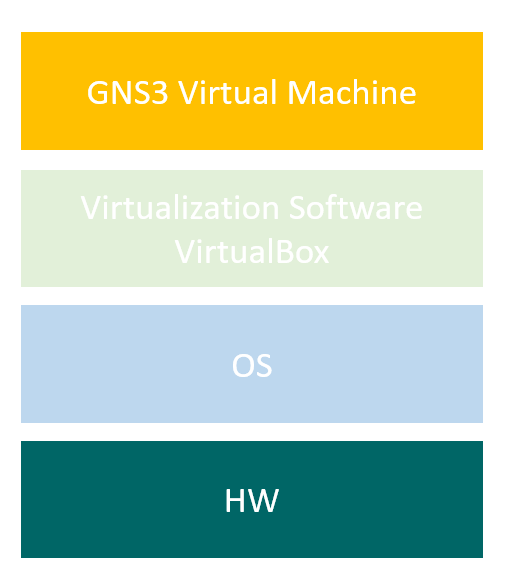
\includegraphics[width=0.5\textwidth]{graphics/Architecture_virtualbox.PNG}
	\caption{\en{Virtualization} Γενική αρχιτεκτονική}
\end{figure}

\begin{figure}[htb]
	\centering
	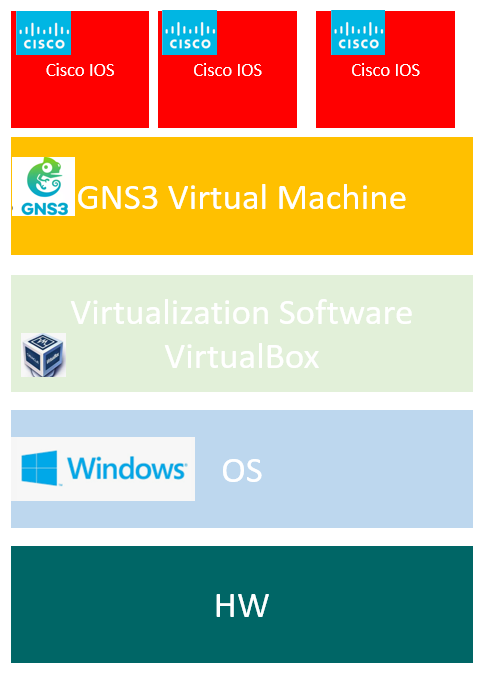
\includegraphics[width=0.5\textwidth]{graphics/virtualization_architecture.PNG}
	\caption{\en{Virtualization} Γενική αρχιτεκτονική}
\end{figure}

\section{Πρόγραμμα εικονοποίσης για το \en{GNS3 VM-VirtualBox}}

Το \en{Oracle VM VirtualBox} ή \en{VirtualBox} (πρώην \en{Sun VirtualBox}, \en{Sun xVM VirtualBox} και \en{Innotek VirtualBox}) είναι υπερεπόπτης
ανοιχτού κώδικα για υπολογιστές \en{x86} που αναπτύσσεται από την \en{Oracle Corporation}.
Αναπτύχθηκε αρχικά από την \en{Innotek GmbH}
και αποκτήθηκε από τη \en{Sun Microsystems} το 2008, η οποία εξαγοράστηκε από την \en{Oracle} το 2010.

Το \en{VirtualBox} μπορεί να εγκατασταθεί σε διάφορα λειτουργικά συστήματα, συμπεριλαμβανόμενων των \en{Linux, macOS, Windows, Solaris} και \en{OpenSolaris}.
Υπάρχουν επίσης μεταφορές για το \en{FreeBSD} και το \en{Genode}.
Υποστηρίζει τη δημιουργία και τη διαχείριση εικονικών μηχανών που εκτελούν εκδόσεις και παραλλαγές των \en{Microsoft Windows, Linux, BSD, Solaris, Haiku, OSx86}
και άλλα, καθώς και περιορισμένη εικονικοποίηση \en{macOS}.
Για ορισμένα λειτουργικά συστήματα είναι διαθέσιμο ένα πακέτο \en{"Guest Additions"} από μηχανές συσκευών και εφαρμογές συστήματος
που συνήθως βελτιώνει την απόδοση, ειδικά των γραφικών, επίσης δίνει την δηνατότητα στον χρήστη να μεταφέρει αρχεία ή κείμενο από μία εικονική μηχανή στον υπολογιστή του χρήστη και να αυξήσει την ανάλυση του παράθυρου της μηχανή. 
Στην εικόνα 3.4 μπορούμε να δούμε το \en{VirtualBox} και την εικονική μηχανή \en{GNS3 VM}

\begin{figure}[htb]
	\centering
	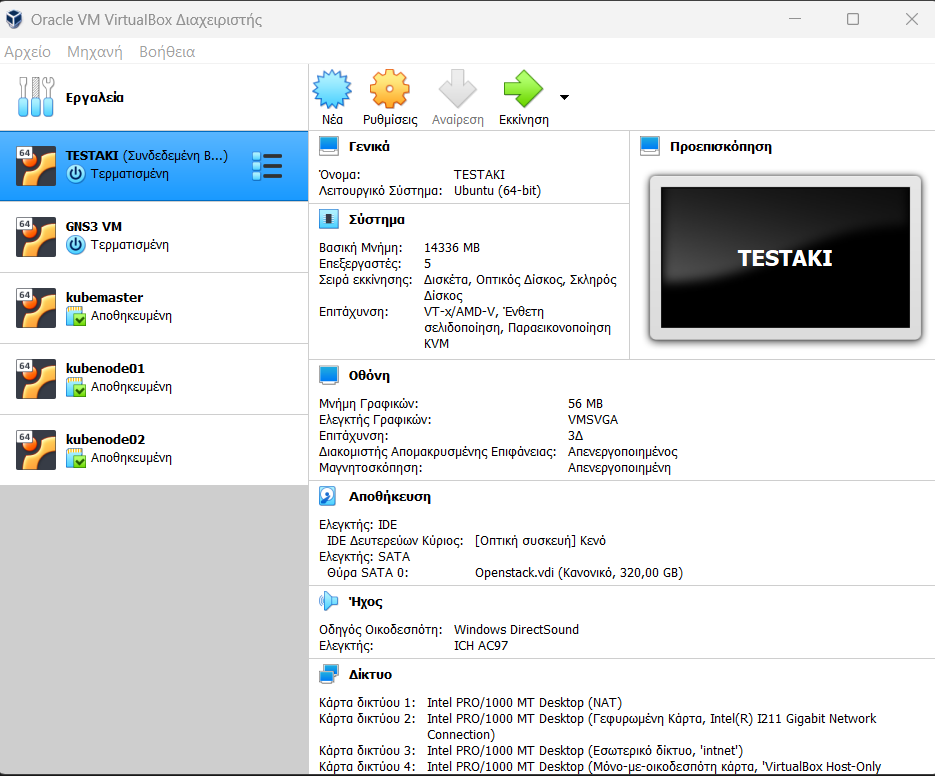
\includegraphics[width=0.9\textwidth]{graphics/virtualbox.PNG}
	\caption{\en{Virtualbox} }
\end{figure}


%\begin{equation}
%	y = \alpha x + \beta
%\end{equation}

%Αντίθετα με αυτό που θεωρεί η πλειοψηφία, το \en{Lorem Ipsum} δεν είναι απλά ένα τυχαίο κείμενο. Οι ρίζες του βρίσκονται σε ένα κείμενο Λατινικής λογοτεχνίας του 45 π.Χ., φτάνοντας την ηλικία του πάνω από 2000 έτη.


%\begin{figure}[htb]
%	\centering
%	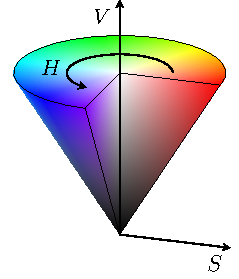
\includegraphics{tikz/hsv_cone/hsv_cone.pdf}
%	\caption{Ο χρωματικός χώρος \en{HSV}.}
%\end{figure}

%\chapter{Τεχνολογιές}

\section{Εισαγωγή}

Αρχικά δημιουργήθηκε η βασική δομή και η δομή της διαδικτυακής πύλης καθορίστηκε. Αυτή η βασική δομή φαίνεται στο Παρακάτω σχήμα

Είναι σημαντικό να σημειωθεί ότι ολόκληρη η εφαρμογή Django βρίσκεται στον ίδιο φυσικό
διακομιστή. Όταν ο χρήστης στέλνει ένα αίτημα για την εκτέλεση ενός σεναρίου με συγκεκριμένες εισόδους αυτό στέλνεται στις συσκευές στο τοπικό δίκτυο.


Το πρώτο βήμα στη διαδικασία ήταν να καθοριστεί τι θα αυτοματοποιηθεί με βάση τις
διάφορες εκτιμήσεις. Για να καθοριστεί αυτό, πραγματοποιήθηκαν πολλές συναντήσεις καταιγισμού ιδεών.
με την ομάδα. Προτού γίνει αυτό όμως η αρχική ιδεά που τέθηκε στο τραπέζι βγήκε με βάση μια παρόμοια δουλειά ενός μηχανικού
της \en{Cisco}. Το έργο του θα αναφερθεί αναλυτικά στην εκτενή βιβλιογραφία στο τέλος. Με βάση λοιπόν
αυτο το έργο ξεκινήσαν συζητήσεις για το πως θα μπορέσουμε να αναπτύξουμε κάτι παρόμοιο
καθώς και να το εμπλουτίσουμε στο τέλος έτσι ώστε να αντοπρίνεται όσο γίνεται στις τεχνολογίες του
σήμερα.

Σε αυτές τις συναντήσεις που γίνανε μεταξύ μας τέθηκαν πολλές ιδέες τέθηκαν στο τραπέζι και η ομάδα καθόρισε
μια σειρά προτεραιότητας για την ανάπτυξη. Ο στόχος σε πολλούς αυτοματισμούς είναι να μειωθεί ο χρόνος που καταναλώνεται για την εκτέλεση
αυτές τις επαναλαμβανόμενες εργασίες. Πολλές τεχνολογίες χρησιμοποιήθηκαν για την υλοποίηση του συγκεκριμένου έργου οι οποίες θα παρουσιαστούν
εκτενώς σε άλλες ενότητες.

Η υλοποίησή μιας τέτοιας εφαρμογής είχε κάποιες δυσκολίες. Κυρίως ποιο θα είναι το περιβάλλον στο οποίο
η εφαρμογή θα μπορούσε να τεσταριστεί και υλοποιηθεί. Για αυτό πάρθηκε η απόφαση οι συσκευές με τις οποίες θα τεσταριστεί
και συνάμα θα λειτουργήσει η εφαρμογή θα είναι \en{virtual }συσκευές της \en{Cisco} οι οποίες θα τρέχουν στο \en{GNS3}
και το \en{GNS3} θα μπορεί να επικοινωνεί δικτυακά με τον \en{Django Server} στο τοπικό δίκτυο.
Το στήσιμο όλου του περιβάλλοντος και της εφαρμογής θα αναλυθεί εκτενώς περαιτέρω σε άλλο κεφάλαιο.


\section{\en{GNS3}}
Το \en{GNS3} Είναι ένα εργαλείο προσομοίωσης δικτύων ανοικτού κώδικα που επιτρέπει στους χρήστες να προσομοιώσουν 
σύνθετες τοπολογίες δικτύων στους υπολογιστές τους. Μηχανικοί δικτύων και φοιτητές 
το χρησιμοποιούν ευρέως για να μάθουν και να εξασκηθούν σε έννοιες δικτύωσης, να δοκιμάσουν διαμορφώσεις δικτύου και να δημιουργήσουν εικονικά περιβάλλοντα δικτύου.


Το \en{GNS3} υποστηρίζει διάφορες συσκευές δικτύου, όπως δρομολογητές, μεταγωγείς και τείχη προστασίας 
από διάφορους προμηθευτές, συμπεριλαμβανομένων των \en{Cisco}, \en{Juniper}, \en{Nokia} και άλλων. Επιτρέπει στους χρήστες να 
προσομοιώσουν διάφορα σενάρια και διαμορφώσεις δικτύου και να δοκιμάσουν τη συμπεριφορά των 
συσκευών δικτύου σε ένα ελεγχόμενο περιβάλλον. 

\begin{figure}[htb]
	\centering
	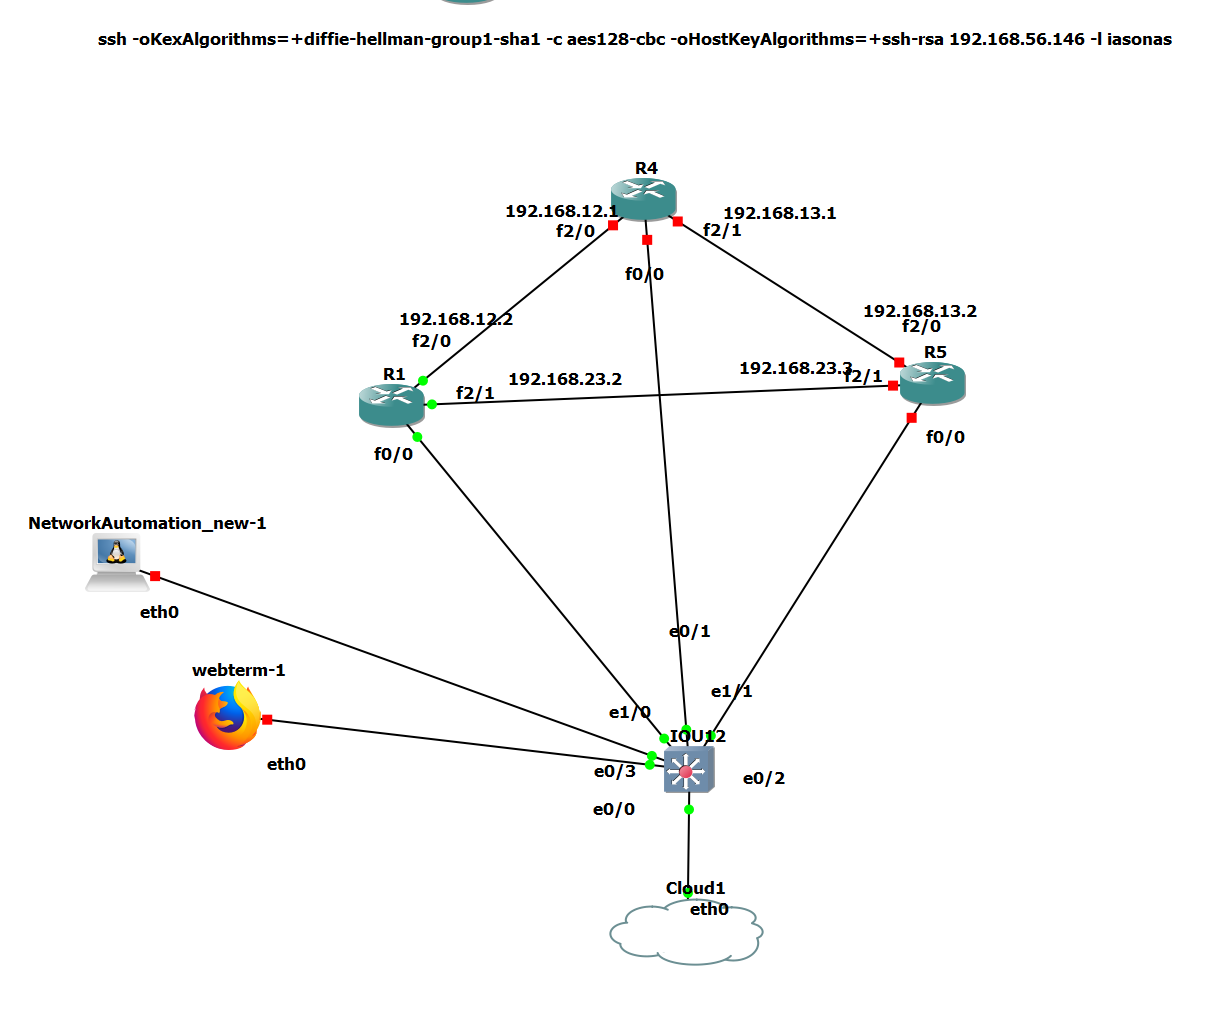
\includegraphics[width=0.7\textwidth]{graphics/Network_topology.png}
	\caption{\en{General Network Topology} }
\end{figure}



\section{\en{Cisco IOS}}
Το \en{IOU} σημαίνει \en{IOS on Unix} είναι μια εικονική έκδοση του λογισμικού \en{IOS} της \en{Cisco} που 
μπορεί να χρησιμοποιηθεί για σκοπούς προσομοίωσης και δοκιμής δικτύου. Επιτρέπει στους μηχανικούς δικτύου να δημιουργούν εικονικές τοπολογίες δικτύου και να εξασκούνται σε διάφορες εργασίες δικτύου, 
όπως η διαμόρφωση δρομολογητών και μεταγωγέων, χωρίς να απαιτείται φυσικό υλικό. Το πλεονέκτημα του \en{GNS3} σε σχέση με εφαρμογές άλλες όπως το \en{Packet tracer} είναι ότι το \en{GNS3} 
μπορεί να σηκώσει πραγματικά \en{images} άρα πραγματικό λογισμικό συνεπώς οι λειτουργίες που μπορείς να κάνεις είναι πολύ περισσότερες.

Το \en{Cisco IOU} χρησιμοποιείται συχνά σε συνδυασμό με λογισμικό προσομοίωσης δικτύου όπως 
\en{GNS3} ή \en{EVE-NG}, τα οποία αποτελούν την πλατφόρμα εικονικοποίησης δικτύου που σας επιτρέπει να 
να δημιουργείτε και να διαχειρίζεστε εικονικά περιβάλλοντα δικτύου για σκοπούς δοκιμής και εκμάθησης, τα οποία παρέχουν ένα γραφικό περιβάλλον χρήστη για τη δημιουργία και τη διαχείριση εικονικών 
τοπολογιών δικτύου. Οι εικόνες \en{IOU} μπορούν να φορτωθούν σε αυτά τα εργαλεία προσομοίωσης για τη δημιουργία εικονικών συσκευών \en{Cisco} που μπορούν να διαμορφωθούν και να δοκιμαστούν όπως το φυσικό δίκτυο 
συσκευές.

\section{Εικονικοποίηση}
Στην επιστήμη της πληροφορικής, η εικονικοποίηση \en{virtualization} είναι ένας ευρύς όρος 
των υπολογιστικών συστημάτων που αναφέρεται σε έναν μηχανισμό αφαίρεσης, 
στοχευμένο στην απόκρυψη λεπτομερειών της υλοποίησης και της κατάστασης
ορισμένων υπολογιστικών πόρων από πελάτες των πόρων αυτών 
(π.χ. εφαρμογές, άλλα συστήματα, χρήστες κλπ). 
Η εν λόγω αφαίρεση μπορεί είτε να αναγκάζει έναν πόρο να 
συμπεριφέρεται ως πλειάδα πόρων (π.χ. μία συσκευή αποθήκευσης σε διακομιστή τοπικού δικτύου),
είτε πολλαπλούς πόρους να συμπεριφέρονται ως ένας (π.χ. συσκευές αποθήκευσης σε κατανεμημένα συστήματα). 

Η εικονικοποίηση δημιουργεί μία εξωτερική διασύνδεση η οποία αποκρύπτει την 
υποκείμενη υλοποίηση (π.χ. πολυπλέκοντας την πρόσβαση από διαφορετικούς χρήστες).
Αυτή η προσέγγιση στην εικονικοποίηση αναφέρεται ως εικονικοποίηση πόρων. 
Μία άλλη προσέγγιση, ίδιας όμως νοοτροπίας, είναι η εικονικοποίηση πλατφόρμας,
όπου η αφαίρεση που επιτελείται προσομοιώνει ολόκληρους υπολογιστές. Το αντίθετο της εικονικοποίησης είναι η διαφάνεια: 
ένας εικονικός πόρος είναι ορατός, αντιληπτός, αλλά στην πραγματικότητα ανύπαρκτος, 
ενώ ένας διαφανής πόρος είναι υπαρκτός αλλά αόρατος. 
 
Θα εξηγήσουμε την εικονικοποίηση στην δικιά μας περίπτωση. Το πρώτο επίπεδο είναι αυτό του υλικού. Η εικονικοποίηση
σα τεχνολογία εικονοποιεί το υλικό για να μπορέσει να δώσε πόρους στις εικονικές μηχανές. Η υλοιποίηση
της εικονικοποίησης γίνεται με λογισμικό \en{hypervisor}. Στη δικιά μας περίπτωση ο \en{hypervisor} είναι 
το \en{Virtual Box} ο οποίος είναι ένας τύπου Β \en{hypervisor}. Ο \en{hypervisor} τύπου 2 είναι μια εφαρμογή εγκατεστημένη 
στο λειτουργικό σύστημα του κεντρικού υπολογιστή το οποίο μας δίνει τη δυνατότητα να σηκώσουμε 
εικονικές μηχανές άλλων λειτουργικών συστημάτων πάνω στο ήδη υπάρχον σύστημα.

Οι παρακάτω εικόνες μπορούν να εξηγήσουν σχηματικά τη γενική καθώς και την ειδική αρχιτεκτονική.

\begin{figure}[htb]
	\centering
	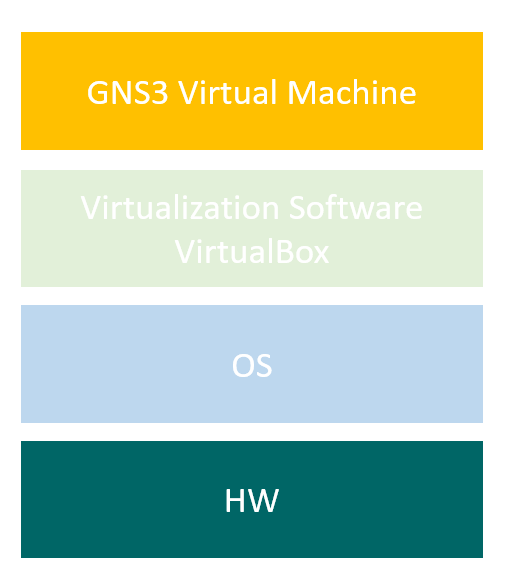
\includegraphics[width=0.5\textwidth]{graphics/Architecture_virtualbox.PNG}
	\caption{\en{Virtualization} Γενική αρχιτεκτονική}
\end{figure}

\begin{figure}[htb]
	\centering
	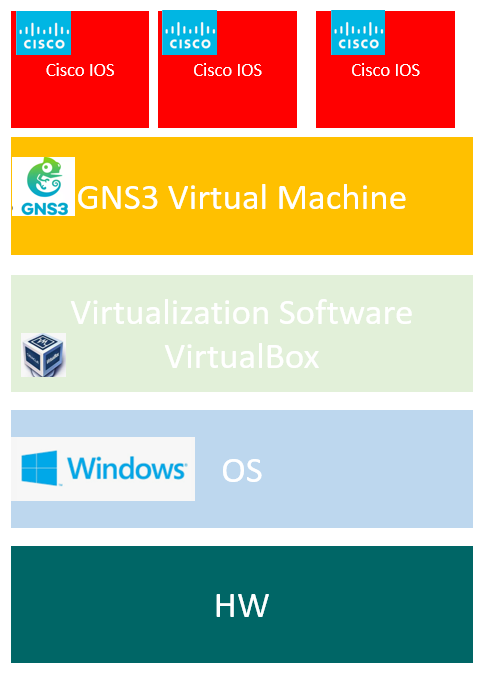
\includegraphics[width=0.5\textwidth]{graphics/virtualization_architecture.PNG}
	\caption{\en{Virtualization} Γενική αρχιτεκτονική}
\end{figure}

\section{Πρόγραμμα εικονοποίσης για το \en{GNS3 VM-VirtualBox}}

Το \en{Oracle VM VirtualBox} ή \en{VirtualBox} (πρώην en{Sun VirtualBox}, \en{Sun xVM VirtualBox} και \en{Innotek VirtualBox}) είναι υπερεπόπτης
ανοιχτού κώδικα για υπολογιστές \en{x86} που αναπτύσσεται από την \en{Oracle Corporation}.
Αναπτύχθηκε αρχικά από την \en{Innotek GmbH}
και αποκτήθηκε από τη \en{Sun Microsystems} το 2008, η οποία εξαγοράστηκε από την \en{Oracle} το 2010.

Το \en{VirtualBox} μπορεί να εγκατασταθεί σε διάφορα λειτουργικά συστήματα, συμπεριλαμβανόμενων των \en{Linux, macOS, Windows, Solaris} και \en{OpenSolaris}.
Υπάρχουν επίσης μεταφορές για το \en{FreeBSD} και το \en{Genode}.
Υποστηρίζει τη δημιουργία και τη διαχείριση εικονικών μηχανών που εκτελούν εκδόσεις και παραλλαγές των \en{Microsoft Windows, Linux, BSD, Solaris, Haiku, OSx86}
και άλλα, καθώς και περιορισμένη εικονικοποίηση \en{macOS}.
Για ορισμένα λειτουργικά συστήματα είναι διαθέσιμο ένα πακέτο \en{"Guest Additions"} από μηχανές συσκευών και εφαρμογές συστήματος
που συνήθως βελτιώνει την απόδοση, ειδικά των γραφικών, επίσης δίνει την δηνατότητα στον χρήστη να μεταφέρει αρχεία ή κείμενο από μία εικονική μηχανή στον υπολογιστή του χρήστη και να αυξήσει την ανάλυση του παράθυρου της μηχανή. 
Στην εικόνα 3.4 μπορούμε να δούμε το \en{VirtualBox} και την εικονική μηχανή \en{GNS3 VM}

\begin{figure}[htb]
	\centering
	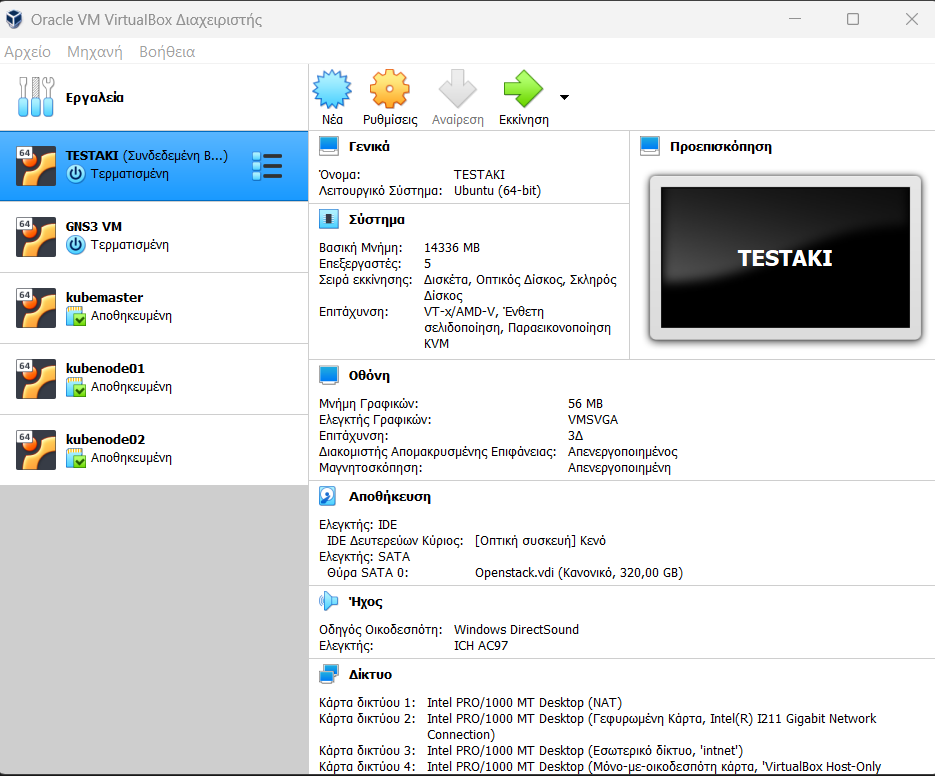
\includegraphics[width=0.9\textwidth]{graphics/virtualbox.PNG}
	\caption{\en{Virtualbox} }
\end{figure}

\section{\en{Django Web Framework}}

Το \en{Django} είναι ένα \en{backedn framework} το οποίο βασίζεται στη γλώσσα προγραμματισμού \en{Python}. Με το \en{Django}, μπορείτε να μεταφέρετε τις εφαρμογές Ιστού από την ιδέα στην κυκλοφορία μέσα σε λίγες ώρες. Το \en{Django} φροντίζει για μεγάλο μέρος
της ταλαιπωρίας της ανάπτυξης ιστού, ώστε να μπορείτε να εστιάσετε στη σύνταξη της εφαρμογής σας χωρίς να χρειάζεται να ανακαλύψετε ξανά τον τροχό.
Είναι δωρεάν και ανοιχτού κώδικα. Ορισμένες από τις πιο μεγάλες εταιρίες στον πλανήτη χρησιμοποιούν την ικανότητα του
να κλιμακώνεται γρήγορα και με ευελιξία για να ανταποκρίνεται στις μεγαλύτερες απαιτήσεις κίνησης. Στη δικιά μας περίπτωση χρησιμοποιήθηκε το συγκεκριμένου
{Framework} γιατί θα μας έδινε τη δυνατότητα να φτιάξουμε μία εφαρμογή με μεγάλη επεκτασιμότητα και παράλληλα να μπορέσουμε να ενσωματώσουμε μεσα διαφορετικές τεχνολογίες.

Παράλληλα με το \en{Django} χρησιμοποιήθηκαν έτοιμες βιβλιοθήκες της \en{Python} προκειμένου να μπορέσουν να εκτελεστούν βασικές λειτουργίες της εφαρμογής όπως 
τα πρωτοκολλα επικοινωνίας. Θεωρούμε ότι η δημιουργία τέτοιων βιβλιοθηκών ξεφεύγει από τα όρια μιας διπλωματικής εργασίας καθώς απαιτεί πολύ χρόνο και ερευνητική
ενασχόληση που μόνο στα πλαίσια ενός διδακτορικού θα μπορούσε να υλοποιηθεί μιά τέτοια ιδέα. Παρακάτων παρουσιάζονται οι βιβλιοθήκες που χρησιμοποιήθηκαν και κάποια βασικά χαρακτηριστικά τους.

\subsection{\en{Paramiko}}
Το \en{Paramiko} είναι μια διασύνδεση καθαρά \en{Python} που υλοποιεί το πρωτόκολλο \en{SSH} έκδοσης 2 σε \en{Python}, παρέχοντας λειτουργικότητα τόσο πελάτη όσο και διακομιστή.
Το \en{Paramiko} μπορεί να επιτύχει υψηλές επιδόσεις σε χαμηλού επιπέδου κρυπτογραφικές έννοιες.
Οποιαδήποτε συσκευή που μπορεί να ρυθμιστεί μέσω \en{SSH} μπορεί επίσης να ρυθμιστεί από την \en{Python} με σενάρια με τη χρήση αυτής της μονάδας.

\subsection{\en{Netmiko}}
Το \en{Netmiko} είναι μια βιβλιοθήκη ανοικτού κώδικα για πολλούς προμηθευτές, που σημαίνει ότι πολλές συσκευές μπορούν να ρυθμιστούν από την \en{python}
χρησιμοποιώντας το \en{Netmiko}.
Ορισμένες από τις συσκευές που υποστηρίζει το \en{Netmiko} είναι οι εξής: \en{Cisco IOS}, \en{Juniper}, \en{Arista}, \en{HP} και \en{Linux}. 
Μπορεί επίσης να υποστηρίζει και άλλους προμηθευτές όπως η \en{Alcatel}, η \en{Huawei} και η \en{Ubiquity} αλλά περιορισμένα 
δοκιμές έχουν γίνει με αυτούς τους προμηθευτές.
Το \en{Netmiko} τρέχει πάνω από το \en{Paramiko} για να κάνει τη σύνδεση \en{SSH} σε συσκευές δικτύου λιγότερο περίπλοκη, πιο ευέλικτη και πιο εύκολη στη χρήση. Παρόλο που το \en{Netmiko} είναι ευκολότερο στη χρήση, όπως αναφέρθηκε 
παραπάνω, υποστηρίζει συγκεκριμένους προμηθευτές και μόνο έναν αριθμό συσκευών τους. Από την άλλη πλευρά,
το \en{Paramiko} μπορεί να χρησιμοποιηθεί για την επικοινωνία με οποιαδήποτε συσκευή που υποστηρίζει \en{SSH}.
Τόσο το \en{Paramiko}όσο και το \en{Netmiko} αποτελούν εναλλακτικές επιλογές για συσκευές που δεν υποστηρίζουν 
\en{APIs}.

\subsection{\en{Napalm}}
Το \en{NAPALM} (\en{Network Automation and Programmability Abstraction Layer with Multivendor support}) είναι μια βιβλιοθήκη \en{Python} που υλοποιεί ένα σύνολο λειτουργιών για την αλληλεπίδραση με διαφορετικά λειτουργικά συστήματα συσκευών δικτύου χρησιμοποιώντας ένα ενοποιημένο \en{API}.
Το \en{NAPALM} υποστηρίζει διάφορες μεθόδους σύνδεσης με τις συσκευές, χειρισμού των ρυθμίσεων ή ανάκτησης δεδομένων. Το \en{Napalm} συνεπώς είναι μια βιβλιοθήκη \en{Python} που παρέχει ένα \en{API}
\en{(Application Programming Interface)} για την εργασία με συσκευές δικτύου. Έχει σχεδιαστεί για να απλοποιεί την
αυτοματοποίηση και τη διαχείριση του δικτύου με την αφαίρεση των υποκείμενων λεπτομερειών που σχετίζονται με τον εκάστοτε προμηθευτή και την παροχή μιας συνεπούς διεπαφής σε διαφορετικά δίκτυα. 
συσκευών.
Το \en{Napalm} επιτρέπει στους μηχανικούς και τους διαχειριστές δικτύων να αυτοματοποιούν κοινές εργασίες διαχείρισης δικτύου, όπως η διαμόρφωση, η παροχή, η παρακολούθηση και η 
αντιμετώπιση προβλημάτων. Υποστηρίζει πολλούς προμηθευτές συσκευών δικτύου, συμπεριλαμβανομένων των \en{Cisco}, \en{Juniper}, \en{Arista} και \en{Huawei}.
Το \en{Napalm} παρέχει ένα σύνολο κοινών λειτουργιών που μπορούν να εκτελεστούν σε συσκευές δικτύου, όπως η ανάκτηση πληροφοριών διαμόρφωσης, η εφαρμογή διαμόρφωσης 
αλλαγών, έλεγχος στατιστικών στοιχείων διασύνδεσης και συλλογή πληροφοριών τοπολογίας δικτύου παρέχει επίσης χαρακτηριστικά όπως υποστήριξη επαναφοράς, επικύρωση διαμόρφωσης 
αλλαγών διαμόρφωσης, και σύγκριση των διαφορών διαμόρφωσης μεταξύ συσκευών.
14
Το \en{Napalm} μπορεί να συνδυαστεί με βιβλιοθήκες \en{Python} όπως οι \en{Netmiko}, \en{Paramiko} και \en{Ansible} για τη δημιουργία σύνθετων ροών εργασίας αυτοματισμού δικτύου. Μπορεί επίσης να ενσωματωθεί 
με δημοφιλή εργαλεία παρακολούθησης δικτύου, όπως το \en{Prometheus} και το \en{Grafana}, για την παρακολούθηση της απόδοσης του δικτύου σε πραγματικό χρόνο.







\chapter{Σχεδίαση και Ανάλυση}

\section{Απαιτήσεις Συστήματος}




\subsection{Λειτουργικές απαιτήσεις}

Μια σειρά από λειτουργίες κρίθηκαν απαραίτητες και υλοποιηθήκαν στην παρούσα εφαρμογή. Έτσι:

\begin{itemize}
    \item Η εφαρμογή διαχείρισης του δικτύου θα πρέπει να  παρέχει στον χρήστη ένα γραφικό περιβάλλον που θα του επιτρέπει να αλληλεπιδρά εύκολα και αποδοτικά με το σύστημα. 
    \item Ο χρήστης θα πρέπει να έχει την δυνατότητα να παρακολουθεί την κατάσταση μιας συγκεκριμένης διεπαφής δικτύου, βλέποντας αν λειτουργεί σωστά ή αν υπάρχουν προβλήματα. 
    \item Επιπλέον, θα πρέπει να έχει τη δυνατότητα να βλέπει αναλυτικά στατιστικά στοιχεία για μια συγκεκριμένη δικτυακή συσκευή, όπως η χρήση δεδομένων, η ταχύτητα σύνδεσης ή τυχόν σφάλματα, αλλά και για συγκεκριμένες διεπαφές του δικτύου, ώστε να κατανοεί τη λειτουργία τους σε βάθος
    \item Η εφαρμογή θα επιτρέπει επίσης τη δημιουργία αντιγράφου ασφαλείας (\en{backup}) της τρέχουσας ρύθμισης του δικτύου, για να μπορεί ο χρήστης να επαναφέρει τη ρύθμιση αν χρειαστεί
    \item Τέλος, θα δίνεται η δυνατότητα αλλαγής της διεύθυνσης \en{IP} μιας επιλεγμένης δικτυακής εφαρμογής, εξασφαλίζοντας μεγαλύτερη ευελιξία στη διαχείριση του δικτύου. 
\end{itemize}

Όλες αυτές οι λειτουργίες έχουν σχεδιαστεί για να διευκολύνουν τη διαχείριση και την παρακολούθηση του δικτύου, ακόμα και από χρήστες χωρίς εξειδικευμένες γνώσεις.


\section{Αρχιτεκτονική της εφαρμογής}

Στην αρχή, οι εφαρμογές ιστού δεν ήταν τίποτα περισσότερο από ένα σύνολο αρχείων \en{HTML, CSS} και
\en{javascript} που ήταν συνδεδεμένα μεταξύ τους. Ένας καλός προγραμματιστής ήταν σε θέση να φτιάξει σπουδαίες εφαρμογές ιστού αν αυτός/αυτή
είχε αρκετές δεξιότητες/γνώσεις.

Στην εποχή μας, εμφανίστηκαν τα \en{frameworks} και λαμβάνοντας υπόψη ότι ουσιαστικά δεν βελτιώνουν αυτό που τελικά βλέπει ο χρήστης και τις
αλληλεπιδράσεις του με το \en{frontend}, τότε
θα μπορούσε κανείς να αναρωτηθεί γιατί χρησιμοποιούνται ευρέως στις μέρες μας.
Παρόμοιες δουλειές με την παρούσα εργασία υπάρχουν και σε άλλες διπλωματικές εργασίες καθώς και σε μη διπλωματικές εργασίες. Μηχανικοί από όλο τον κόσμο
ασχολούνται με την αυτοματοποίηση συστημάτων και τη δημιουργία κώδικα που να αυτοματοποιεί συσκευές/συστήματα. 

Με βάση άλλες τέτοιες προσπάθειες που έχουν γίνει στο παρελθόν εμείς συλλέξαμε την εως τώρα βιβλιογραφία
και προσπαθήσαμε να φτιάξουμε μία τέτοια εφαρμογή η οποία όμως να βασίζεται στα τωρινά δεδομένα και να 
ενσωματσώσουμε τις τελευταίες τεχνολογίες αιχμής όπως την \en{Cloud Native} αρχιτεκτονική. Στη συνέχεια γίνεται προσπάθεια να δωθεί εκτενής
ανάλυση στο πως λειτουργεί η εφαρμογή καθώς και στην αλληλλεπίδρασή της με τα συνεργαζόμενα συστήματα. 
 
\subsection{Μοντέλο \en{MVC} (\en{Model-View-Controller})}

Το μοτίβο \en{MVC}[15] (\en{Model-View-Controller} σχήμα 5.1) είναι ένα αρχιτεκτονικό πρότυπο ανάπτυξης λογισμικού που έχει ως στόχο τον διαχωρισμό της παρουσίασης των δεδομένων από τη λογική που διέπει τη διαχείριση των αλληλεπιδράσεων του χρήστη. Συγκεκριμένα, το \en{"Model"} αναλαμβάνει τη διαχείριση των δεδομένων και της επιχειρησιακής λογικής, το "\en{View}" είναι υπεύθυνο για την παρουσίαση των δεδομένων στον χρήστη, ενώ το "\en{Controller}" χειρίζεται την αλληλεπίδραση του χρήστη και τη ροή των δεδομένων μεταξύ του \en{Model} και του \en{View}.
Χάρη στη δομή του, το \en{MVC} προσφέρει μεγαλύτερη ευελιξία, επεκτασιμότητα και καλύτερη οργάνωση του κώδικα, καθιστώντας το ιδανικό για σύνθετες εφαρμογές. Γι’ αυτόν τον λόγο, όλα τα κορυφαία \en{frameworks} για την ανάπτυξη εφαρμογών \en{web}, όπως το \en{Django}, είναι βασισμένα σε αυτό το μοτίβο.


\begin{figure}[h]
	\centering
	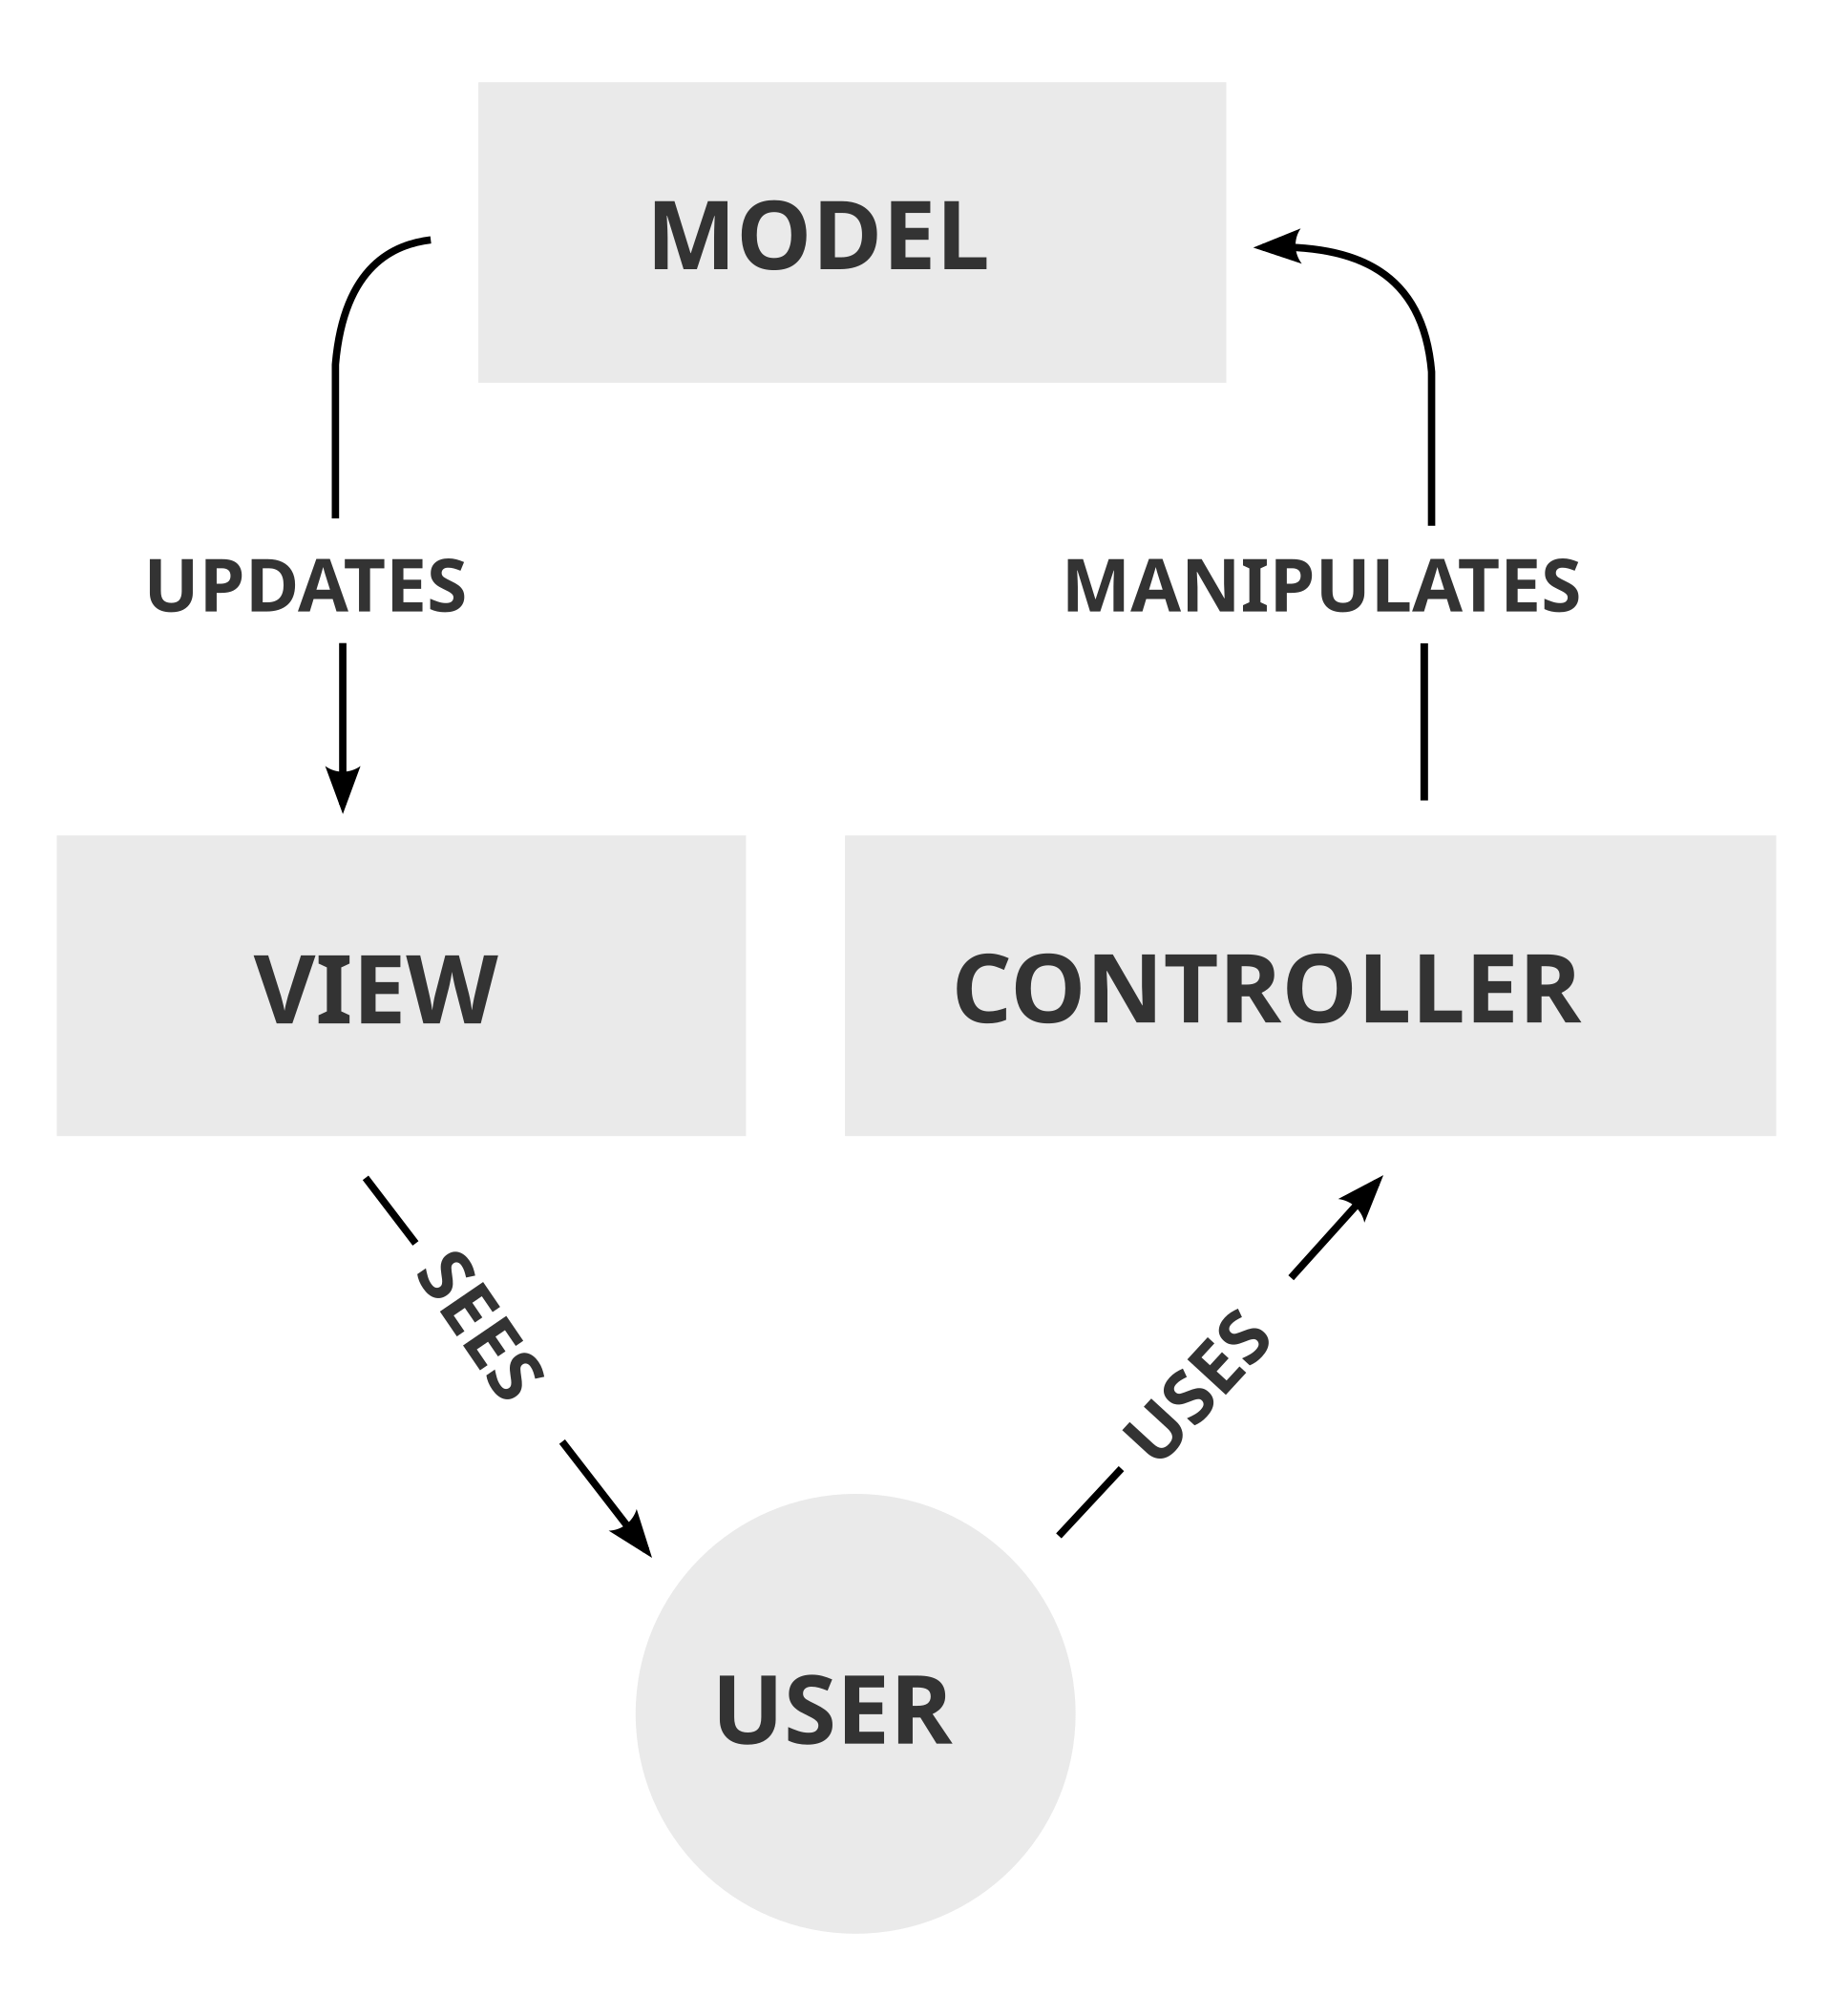
\includegraphics[width=0.7\textwidth]{graphics/MVC-Process.svg.png}
	\caption{\en{MTC} μοντέλο}
\end{figure}

\FloatBarrier

\subsection{\en{Django MTV} }

Παρόλο που το \en{Django} ακολουθεί το μοτίβο \en{MVC}, προτιμά να χρησιμοποιεί τη δική του λογική στην υλοποίηση. Το \en{framework} αναλαμβάνει το \en{Controller} 
μέρος του \en{MVC} και αφήνει τα περισσότερα από τα "καλά" να γίνονται στο \en{Model-Template-View (MTV)}.
Αυτός είναι ο λόγος που το \en{Django} συχνά αναφέρεται ως \en{MTV framework}.



\subsection{Χρήση του \en{MTV} στην εφαρμογή}

Η εφαρμογή διαχείρισης δικτύου έχει υλοποιηθεί με βάση το 
αρχιτεκτονικό μοτίβο \en{MVC (Model-View-Controller)}, το οποίο 
εξασφαλίζει τη σαφή οργάνωση της λειτουργικότητας της εφαρμογής σε 
τρία επίπεδα: το μοντέλο για τη διαχείριση των δεδομένων, τα πρότυπα 
για την παρουσίαση των πληροφοριών στον χρήστη και τις προβολές για 
τη διασύνδεση των χρηστών με τα δεδομένα και την παρουσίασή τους.
Το μοντέλο αποτελεί τον πυρήνα της εφαρμογής και διαχειρίζεται τα 
δεδομένα που σχετίζονται με τις δικτυακές συσκευές. 

Το βασικό μοντέλο που χρησιμοποιείται εδώ είναι το \en{Device}, 
το οποίο αναπαριστά συσκευές όπως δρομολογητές και \en{switches}, 
αποθηκεύοντας πληροφορίες όπως η διεύθυνση του \en{host}, το όνομα 
χρήστη και ο κωδικός πρόσβασης, η πλατφόρμα της συσκευής 
και πρόσθετα στοιχεία ασφαλείας. Το \en{Device} είναι συνδεδεμένο με 
τη βάση δεδομένων της εφαρμογής και παρέχει τις βασικές λειτουργίες 
για την εισαγωγή, ανάγνωση, επεξεργασία και διαγραφή δεδομένων. 
Αυτή η δομή επιτρέπει την κεντρική διαχείριση όλων των δεδομένων που 
απαιτούνται για την ομαλή λειτουργία της εφαρμογής.

Για την παρουσίαση των δεδομένων στον χρήστη, χρησιμοποιούνται αρχεία 
\en{HTML} ως πρότυπα. Αυτά τα αρχεία λειτουργούν ως δυναμικές σελίδες 
που δημιουργούνται με τη γλώσσα \en{Django Template}, εξασφαλίζοντας 
την απεικόνιση των δεδομένων με τρόπο φιλικό προς τον χρήστη. 
Για παράδειγμα, τα πρότυπα χρησιμοποιούνται για την εμφάνιση της λίστας των συσκευών, παρέχοντας λεπτομέρειες για κάθε μία από αυτές, καθώς και για την προβολή στατιστικών ή ρυθμίσεων. Επιπλέον, τα πρότυπα προσαρμόζονται ανάλογα με τα δεδομένα που αντλούνται από το μοντέλο, ώστε να παρέχουν ενημερωμένες πληροφορίες, όπως αποτελέσματα εκτέλεσης εντολών ή την κατάσταση μιας συσκευής.

Οι προβολές της εφαρμογής(\en{views.py}) είναι συναρτήσεις \en{Python} που συνδέουν 
τα αιτήματα των χρηστών με τα δεδομένα και την παρουσίαση. 
Όταν ένας χρήστης κάνει μια ενέργεια, όπως το να ζητήσει την προβολή 
μιας λίστας συσκευών, η αντίστοιχη προβολή λαμβάνει το αίτημα, 
επικοινωνεί με το μοντέλο για να ανακτήσει τα δεδομένα και στη 
συνέχεια τα περνάει στο κατάλληλο πρότυπο. Όλες οι λειτουργικές δυνατότητες της εφαρμογής μας υλοποιούνται μέσα στη σελίδα \en{views.py}.
Το πρότυπο δημιουργεί τη σελίδα \en{HTML} που θα επιστραφεί στον χρήστη, περιέχοντας όλες τις πληροφορίες που ζήτησε. Για παράδειγμα, αν ένας χρήστης θέλει να δει τα στατιστικά μιας συγκεκριμένης συσκευής, η προβολή θα αντλήσει τα απαραίτητα δεδομένα από το μοντέλο και θα τα επιστρέψει στον χρήστη μέσα από ένα προσαρμοσμένο πρότυπο.

Με τον τρόπο αυτό, το μοτίβο \en{MVC} εξασφαλίζει την αποτελεσματική 
λειτουργία της εφαρμογής, διαχωρίζοντας τις ευθύνες ανάμεσα στη 
διαχείριση των δεδομένων, την παρουσίαση τους και την επικοινωνία με τον χρήστη. Η οργάνωση αυτή καθιστά την εφαρμογή ευέλικτη και εύκολη στη συντήρηση, ενώ παράλληλα βελτιώνει την εμπειρία χρήσης, παρέχοντας ένα λειτουργικό και φιλικό περιβάλλον διαχείρισης δικτυακών συσκευών
Στο σχήμα 5.2 παρουσιάζεται διάγραμμα απεικόνισης της βασικής αρχιτεκτονικής της εφαρμογής.

\begin{figure}[h]
	\centering
	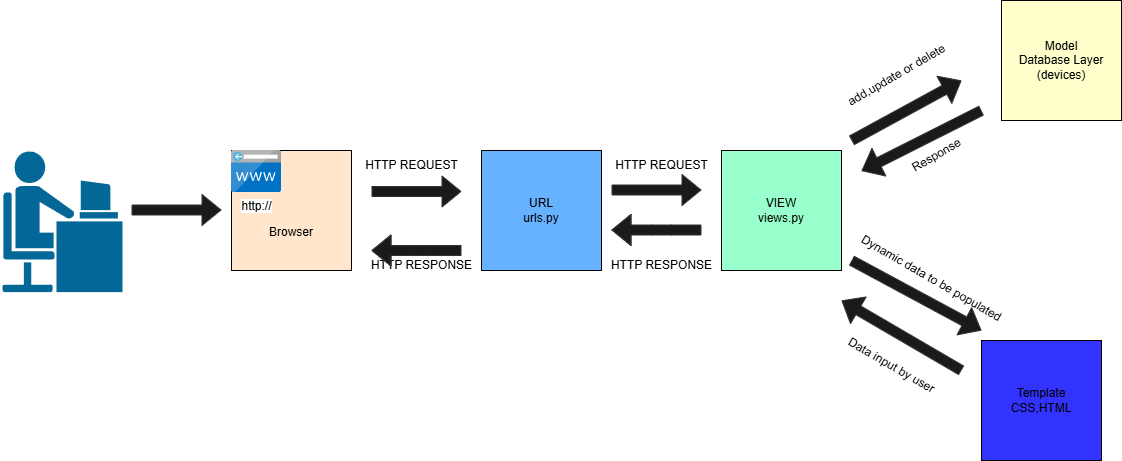
\includegraphics[width=0.7\textwidth]{graphics/MTV.drawio.png}
	\caption{Διαγραμματική απεικόνιση της εφαρμογής}
\end{figure}



\section{Εικονικό Περιβάλλον Δικτύου \en{GNS3 –Testbed}}


Το τοπικό περιβάλλον ανάπτυξης πάνω στο οποίο δοκιµάστηκε η εφαρµογή είναι \en{Linux}, \en{Ubuntu} 22.04.2 \en{LTS} η οποία εικονοποιήθηκε πάνω σε λειτουργκό \en{Windows} ως \en{WSL2}. Το \en{Windows Subsystem for Linux version 2}[11] είναι µια τεχνολογία της \en{Microsoft} που επιτρέπει στους χρήστες \en{Windows} να τρέχουν \en{Linux} περιβάλλοντα απευθείας στο λειτουργικό σύστηµα \en{Windows}, χωρίς την ανάγκη για εξοµοιωτές ή εικονικές µηχανές. Είναι η δεύτερη έκδοση του \en{Windows Subsystem for Linux} και αποτελεί σηµαντική βελτίωση σε σχέση µε την πρώτη έκδοση \en{WSL1}. Το \en{WSL 2} χρησιµοποιεί την τεχνολογία εικονικοποίησης (\en{virtualization}) για να τρέχει έναν πραγµατικό πυρήνα \en{Linux} µέσα σε µια ελαφριά εικονική µηχανή βοηθητικών λειτουργιών (\en{utility VM}). Αυτό επιτρέπει στο \en{WSL 2} να προσφέρει καλύτερη απόδοση, πλήρη συµβατότητα µε τις λειτουργίες \en{Linux} και πρόσβαση σε εργαλεία όπως το \en{Docker}.


Το \en{WSL2} αξιοποιήθηκε διότι παρέχει τη δυνατότητα λειτουργίας ενός 
περιβάλλοντος \en{Linux} μέσα σε έναν υπολογιστή με λειτουργικό 
σύστημα \en{Windows}, χωρίς να απαιτείται η χρήση ενός \en{Type B Hypervisor}. 
Αυτό καθιστά τη διαδικασία πιο ελαφριά και αποδοτική, επιτρέποντας τη 
δημιουργία και εκτέλεση του \en{Django server} και τη διαχείριση των 
απαιτήσεων που περιλαμβάνονται στο αρχείο \en{requirements.txt} με έναν πιο οργανωμένο και σταθερό τρόπο.

Το αρχείο \en{requirements.txt}[16] είναι ένα αρχείο το οποίο περιέχει τις βιβλιοθήκες της \en{Python} που θα χρησιμοποιήσουμε στην εφαρμογή μας. Είναι ένα \en{text} αρχείο το οποίο περιέχει όλα εκείνα τα στοιχεία του λογισμικού τα οποία είναι απαραίτητα προκειμένου να τρέξει η εφαρμογή μας. Με τη βοήθεια του \en{package manager} της \en{Python} το \en{pip} μπορούμε εύκολα να εγκαταστήσουμε με μία εντολή όλες τις βιβλιοθήκες που έχουμε βάλει μέσα σε αυτό το \en{text} αρχείο. Με την εντολή αυτή \en{pip install -r requirements.txt} εγκαθιστούμε αυτόματα όλο το απαραίτητο λογισμικό προκειμένου να τρέξει η εφαρμογή μας.

Η εξοικείωσή μου με περιβάλλοντα \en{Unix} έπαιξε καθοριστικό ρόλο 
στο να επιλέξω να φτιάξω το περιβάλλον αυτό, καθώς το \en{WSL2} προσφέρει μια 
εμπειρία χρήσης που μοιάζει πολύ με αυτή ενός πλήρους \en{Linux} 
συστήματος. Αυτή η προσέγγιση επέτρεψε τη χρήση γνωστών εργαλείων και 
πρακτικών ανάπτυξης, ενώ ταυτόχρονα αξιοποίησε τη συμβατότητα του \en{Windows} 
οικοσυστήματος το οποίο χρειάστηκε για την εγκατάσταση του \en{GNS3}. Έτσι, επιτεύχθηκε η δημιουργία ενός τοπικού περιβάλλοντος 
ανάπτυξης που συνδυάζει την ευελιξία και τη σταθερότητα των \en{Unix} 
συστημάτων με την ευκολία πρόσβασης που παρέχει το λειτουργικό σύστημα \en{Windows}.

Το γεγονός ότι το \en{WSL2} αποτελεί ένα \en{Linux} περιβάλλον που εκτελείται πάνω σε λειτουργικό σύστημα \en{Windows} είχε καθοριστική σημασία για την παρούσα υλοποίηση. Αυτό οφείλεται στο ότι τόσο το \en{GNS3} όσο και το \en{VirtualBox} εγκαταστάθηκαν στο \en{Windows} περιβάλλον, ενώ το \en{WSL2} αξιοποιήθηκε αποκλειστικά για την ανάπτυξη της εφαρμογής \en{Django}. Αυτή η διάκριση στη χρήση των εργαλείων επέτρεψε την ομαλή ενσωμάτωση του \en{Linux} περιβάλλοντος στο συνολικό σύστημα, διατηρώντας παράλληλα τη συμβατότητα με τις απαιτήσεις της προσομοίωσης δικτύου.

\subsection{Σχεδίαση Τοπολογίας Δικτύου}

Η ανάπτυξη του \en{Testbed} βασίστηκε στη λογική ότι οι συσκευές που εκτελούνται στο \en{GNS3 VM} θα πρέπει να μπορούν να αλληλεπιδρούν με το τοπικό περιβάλλον \en{WSL2}. Για να επιτευχθεί αυτός ο στόχος, ακολουθήθηκε μια συγκεκριμένη μεθοδολογία, η οποία περιλαμβάνει διαδοχικά βήματα.
Το πρώτο και θεμελιώδες βήμα ήταν η εγκατάσταση των απαραίτητων λογισμικών εργαλείων, τα οποία έχουν ήδη παρουσιαστεί στο θεωρητικό υπόβαθρο. Η διαδικασία δημιουργίας του \en{testbed} αποδείχθηκε ιδιαίτερα απαιτητική, γι' αυτό και θα εξηγήσουμε ορισμένες βασικές αρχές που διέπουν τη λειτουργία του, ώστε να γίνει πιο κατανοητή.
Όπως αναφέρθηκε στο προηγούμενο κεφάλαιο, έχουμε ήδη εγκαταστήσει το \en{GNS3}, το \en{GNS3 VM} στο \en{VirtualBox}, και πλέον είμαστε έτοιμοι να διαμορφώσουμε το περιβάλλον όπου οι συσκευές της \en{Cisco}, που εκτελούνται στο \en{GNS3 VM}, θα μπορούν να επικοινωνούν με το \en{WSL2}, το οποίο αποτελεί και το βασικό λειτουργικό σύστημα του πειραματικού μας περιβάλλοντος.


Λόγω των περιορισμένων υπολογιστικών πόρων που διατίθενται στο πλαίσιο αυτής της διπλωματικής εργασίας, η τοπολογία που χρησιμοποιήθηκε είναι απλή, όπως φαίνεται και στο Σχήμα 5.3. Συγκεκριμένα, η δομή του \en{testbed} περιλαμβάνει πρώτον έναν κόμβο \en{Cloud}, ο οποίος επιτρέπει τη δικτυακή αλληλεπίδραση μεταξύ των συσκευών του \en{GNS3 VM} και του \en{WSL2} και μία συσκευή δοκιμών, που χρησιμοποιείται για την αξιολόγηση της συνδεσιμότητας και της επικοινωνίας στο προτεινόμενο περιβάλλον. Επιλέχθηκε αυτή η τοπολογία διότι αυτή είναι ικανή να μας προσφέρει με το ελάχιστο δυνατό υπολογιστικό κόστος το απαραίτητο περιβάλλον που θα τεστάρουμε.
Με αυτήν την προσέγγιση, διασφαλίζεται η σωστή λειτουργία του \en{testbed}, καθιστώντας εφικτή τη μελέτη και την ανάλυση της επικοινωνίας μεταξύ των εικονικών και των φυσικών συσκευών.

\FloatBarrier

\begin{figure}[htb]
	\centering
	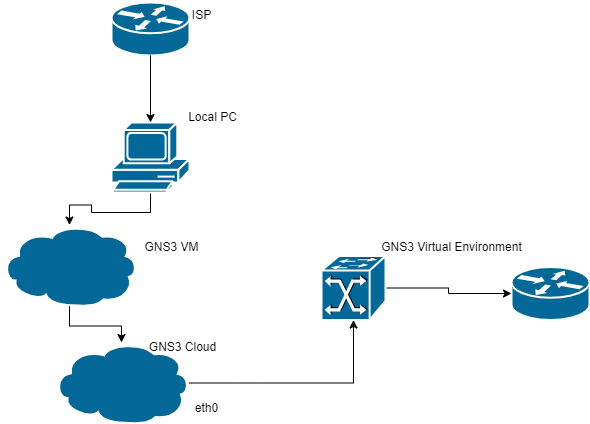
\includegraphics[width=0.7\textwidth]{graphics/diagram.drawio.png}
	\caption{\en{Local PC-GNS3VM-CISCO IOS Connection Architecture} }
\end{figure}

\FloatBarrier

Το \en{GNS3 cloud node} μας δίνει τη δυνατότητα να συνδέσουμε τις συσκευές μας που τρέχουν στο \en{GNS3 VM} με το τοπικό μας δίκτυο. Για να γίνει αυτό ρυθμίζουμε το \en{cloud node} έτσι ώστε to \en{eth0 interface} του να δώσει \en{ip} διεύθυνση μέσα από το \en{DHCP} πρωτόκολλο στα \en{devices} μας. Με αυτόν τον τρόπο έχουμε απευθείας πρόσβαση σε αυτά μέσα από το τοπικό μας δίκτυο.

Για την παραμετροποίηση του \en{Cloud Node}, ρυθμίζουμε το \en{interface} που συνδέεται με τη συσκευή, ακολουθώντας την παρακάτω διαδικασία. Αρχικά, συνδέουμε το \en{interface eth0} του \en{Cloud Node} με το αντίστοιχο \en{eth0} της συσκευής, όπως φαίνεται στην 5.4 εικόνα. 

\FloatBarrier

\begin{figure}[htb]
	\centering
	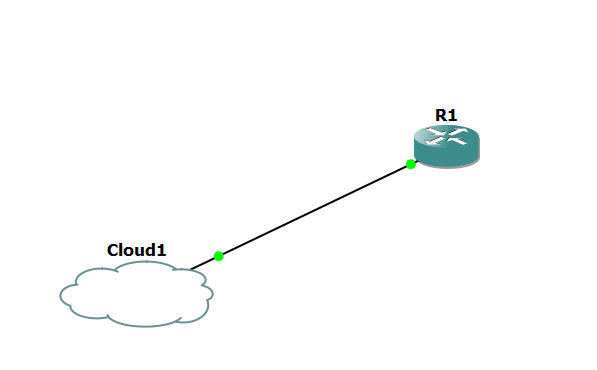
\includegraphics[width=0.7\textwidth]{graphics/CISCO_CLOUD.png}
	\caption{\en{CLOUD NODE With CISCO Node Connection} }
\end{figure}

\FloatBarrier

\noindent Η σύνδεση πραγματοποιείται μέσω της επιλογής του \en{interface} από το \en{Configuration Menu} του \en{Cloud Node}. Συγκεκριμένα, κάνουμε δεξί κλικ στο \en{Cloud Node}, επιλέγουμε "Παραμετροποίηση" και στη συνέχεια προσθέτουμε το \en{eth0} ως τη διεπαφή επικοινωνίας του τοπικού δικτύου με τον διακομιστή όπως φαίνεται στην εικόνα 5.5.

\FloatBarrier

\begin{figure}[htb]
	\centering
	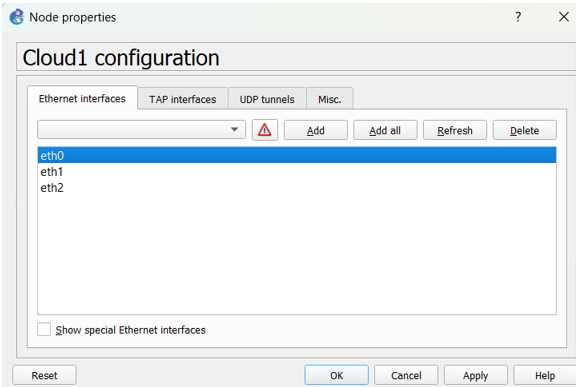
\includegraphics[width=0.7\textwidth]{graphics/CLOUD_NODE_CONFIGURATION.png}
	\caption{\en{CLOUD NODE Configuration} }
\end{figure}

\FloatBarrier


\noindent Η επιλογή του \en{eth0} είναι καθοριστικής σημασίας, καθώς στο \en{GNS3 VM} το συγκεκριμένο \en{interface} είναι ήδη προρυθμισμένο για αυτήν τη λειτουργία, διασφαλίζοντας έτσι την ορθή επικοινωνία του τοπικού δικτύου με τον διακομιστή. Γιατί όμως επιλέγουμε το \en{eth0} στο σχήμα 5.4 και όχι το \en{eth1} ή το \en{eth2}.

Επιλέγουμε το \en{eth0} στο \en{Cloud node} διότι αυτό ανήκει στο δίκτυο της Γεφυρωμένης Κάρτας Δικτύου που επιλέξαμε για το \en{GNS3 VM}. Στην εικόνα παρακάτω(Σχήμα 5.6) βλέπουμε την κάρτα δικτύου του \en{GNS3 VM}.

\FloatBarrier

\begin{figure}[htb]
	\centering
	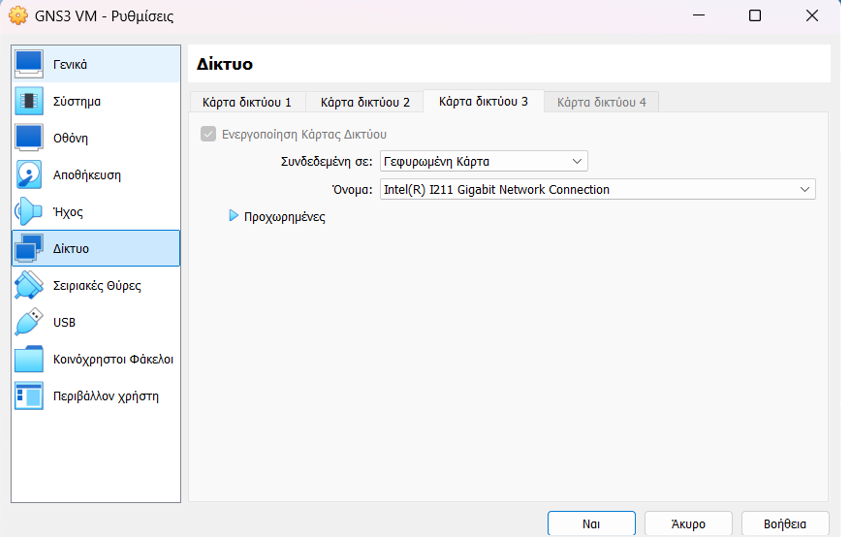
\includegraphics[width=0.7\textwidth]{graphics/GNS3_network_adapter.png}
	\caption{\en{GNS3 VM} κάρτα δικτύου }
\end{figure}

\FloatBarrier

\noindent Προκειμένου να φτιάξουμε την κάρτα δικτύου αυτή μέσα από τα εργαλεία του \en{Vbox} πατάμε Δημιουργία \en{Host-only Networks}
και ρυθμίζουμε την κάρτα δικτύου όπως φαίνεται στο σχήμα 5.7. Στο σχήμα φαίνεται ότι όλες οι συσκευές μας θα πρέπει να παίρνουν \en{IP} διεύθυνση από το δίκτυο 192.168.56.0/24


\FloatBarrier

\begin{figure}[htb]
	\centering
	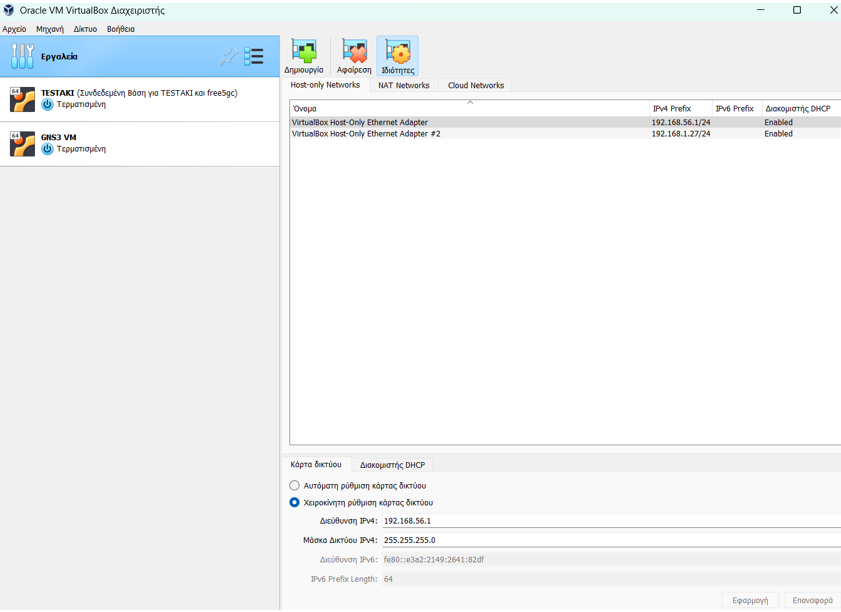
\includegraphics[width=0.7\textwidth]{graphics/GNS3_Network.png}
	\caption{\en{GNS3 VM} δίκτυο }
\end{figure}

\FloatBarrier


\noindent Αφού φτιάξουμε την κάρτα δικτύου του \en{VBox} αυτή μετά φαίνεται αυτόματα στις συνδέσεις δικτύου του υπολογιστή μας όπως στην εικόνα 5.8.

\FloatBarrier

\begin{figure}[htb]
	\centering
	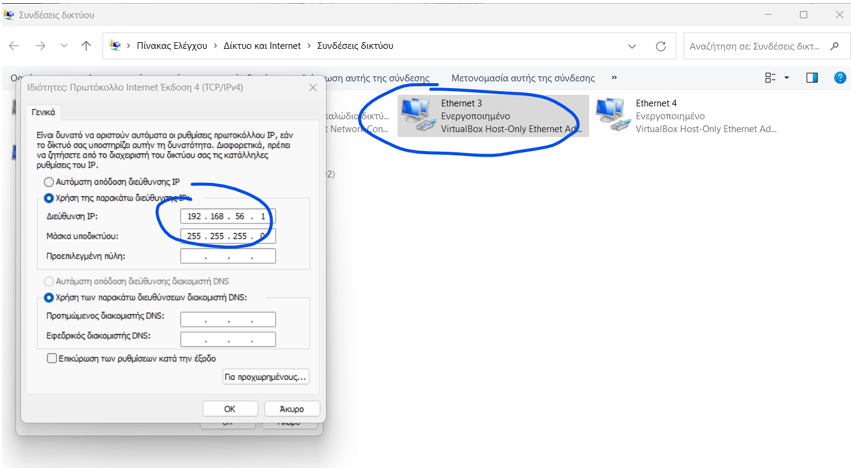
\includegraphics[width=0.7\textwidth]{graphics/windows_host_networking.png}
	\caption{Κάρτα δικτύου στο \en{Windows} λειτουργικό}
\end{figure}

\FloatBarrier

Προκειµένου τώρα οι συσκευές αυτές να µπορέσουν να µιλήσουν µε το τοπικό µας δίκτυο θα πρέπει να τους ορίσουµε \en{IP} διευθύνσεις . Συνεπώς με αυτήν την παραμετροποίηση όταν παραμετροποιήσουμε και τη δικτυακή συσκευή να παίρνει \en{IP} διεύθυνση από αυτό το τοπικό δίκτυο τότε θα μπορούμε από το τοπικό δίκτυο να μιλάμε με στις συσκευές μας για τους \en{testing} λόγους.
Προκειμένου να παίρνουν οι συσκευές \en{IP} διεύθυνση από το τοπικό δίκτυο δηλαδή από το εικονικό \en{interface} του \en{Vbox} που δημιουργήσαμε παραπάνω(192.168.56.0/24) κάναμε την παρακάτω παραμετροποίηση.
Στο σχήμα 5.9 φαίνεται η παραμετροποίηση στην δικτυακή συσκευή.

\FloatBarrier

\begin{figure}[htb]
	\centering
	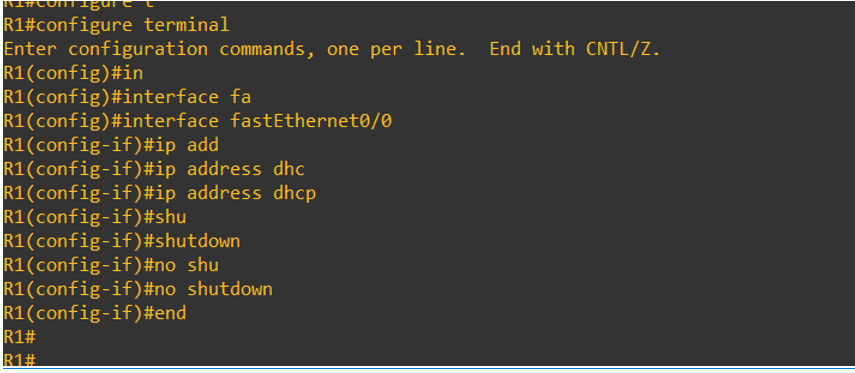
\includegraphics[width=0.7\textwidth]{graphics/cisco_ssh_config_2.png}
	\caption{Παραμετροποίηση στη δικτυακή συσκευή}
\end{figure}

\FloatBarrier

\noindent Στο σχήμα 5.10 φαίνεται η συσκευή να παίρνει σωστά \en{IP} διευθύνση από το 192.168.56.0/24.

\FloatBarrier

\begin{figure}[htb]
	\centering
	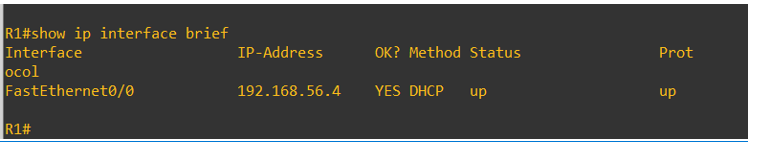
\includegraphics[width=0.7\textwidth]{graphics/cisco_ip_address.png}
	\caption{Κατανομή \en{IP} διευθύνσης}
\end{figure}

\FloatBarrier


\noindent Αφού το \en{interface} πήρε \en{IP} διεύθυνση ελέγχουμε στο τέλος ότι μπορούμε να επικοινωνήσουμε με τη συσκευή όπως στο σχήμα 5.11. Στα σχήματα οι \en{IP} διευθύνσεις μπορεί να είναι διαφορετικές καθώς δοκιμάστηκαν σε διαφορετική φάση. Η ουσία όμως είναι ότι όλες θα παίρνουν \en{IP} διεύθυνση από το δίκτυο 192.168.56.1/24 το οποίο θα αποτελεί και το τελικό δίκτυο πάνω στο οποίο θα αλληλεπιδρούν ο \en{Django Server} με το \en{GNS3 testbed}. Το δίκτυο αυτό είναι κοινό για όλα τα \en{nodes} που βλέπουμε στο Σχήμα 5.3 το οποίο σχεδιάστηκε προκειμένου να γίνει κατανοητή η σχεδίαση.

\FloatBarrier

\begin{figure}[htb]
	\centering
	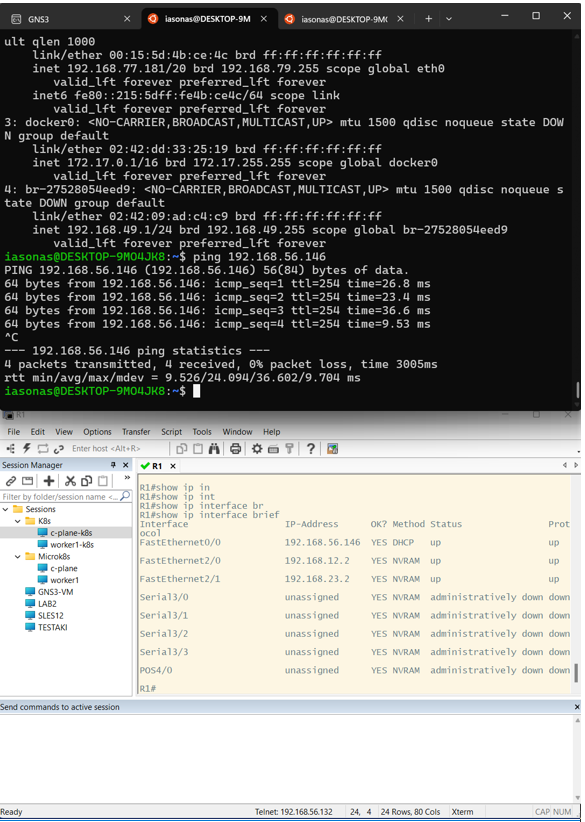
\includegraphics[width=0.7\textwidth]{graphics/ip_connectivity_test.png}
	\caption{\en{IP connectivity test}}
\end{figure}

\FloatBarrier





\subsection{Προσομοίωση Συσκευών \en{Cisco}}

  Προκειμένου να προσομειώσουμε συσκευές της \en{Cisco} το πρώτο βήμα είναι να κατεβάσουμε συγκεκριμένο \en{appliance} απο το \en{GNS3 marketplace}. Αφού το κατεβάσουμε το εισάγουμε στο \en{GNS3} με τον εξής τρόπο: (εικόνα 5.12)

\FloatBarrier

\begin{figure}[htb]
	\centering
	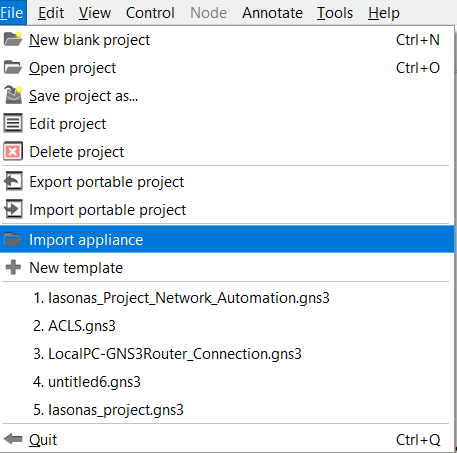
\includegraphics[width=0.7\textwidth]{graphics/import_appliance.png}
	\caption{\en{Import appliance} }
\end{figure}

\FloatBarrier

\noindent Ακολούθως πατάμε \en{Install appliance on the GNS3 VM} και ματσάροντας το \en{filename} του \en{appliance} με το \en{image} που έχουμε μας επιτρέπει να εισάγουμε τη συσκευή. Για να δούμε το \en{filename} στο \en{appliance} ανοίγουμε το αρχείο με έναν \en{editor} και αλλάζουμε το \en{filename} αντίστοιχα οπως στην  εικόνα 5.13.

\FloatBarrier

\begin{figure}[htb]
	\centering
	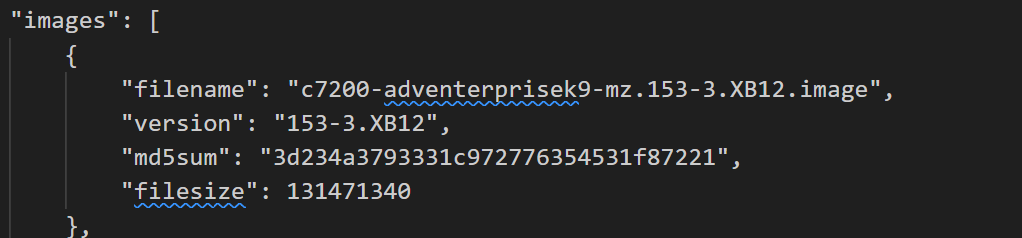
\includegraphics[width=0.7\textwidth]{graphics/appliance_filename.png}
	\caption{\en{filename configuration} }
\end{figure}

\FloatBarrier

Μετά το τέλος της διαδικασίας η συσκευή θα έχει προστεθεί και μπορούμε να την δούμε στην επιλογή \en{Browse all devices}.
Συνεπώς θα μπορούμε να την προσθέσουμε σε τοπολογία και να την κάνουμε να δουλέψει. Για να μπορέσουμε να δουλέψουμε με τη συσκευή θα πρέπει να έχουμε παραμετροποιήσει συγκεκριμένο \en{username},\en{password},\en{secret} καθώς και να τρέχει \en{ssh service}
προκειμένου να μπορούμε να συνδεθούμε μέσα απο το \en{API}. 

Στην  εικόνα 5.14 φαίνεται τι πρέπει να έχει υλοποιηθεί ως προυπόθεση στην εφαρμογή. Φυσικά θεωρούμε δεδομένο ότι έχουν γίνει όλα τα προηγούμενα βήματα καθώς το παρακάτω αφορά μόνο το χρήστη και τον κωδικό του προκειμένου να υλοποιήσει την \en{SSH} σύνδεση.
\FloatBarrier

\begin{figure}[htb]
	\centering
	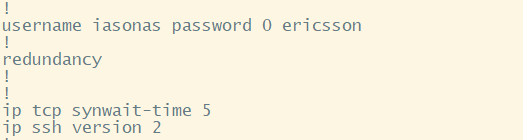
\includegraphics[width=0.7\textwidth]{graphics/ssh.png}
	\caption{\en{ssh and credentials requirements} }
\end{figure}

\FloatBarrier

%\chapter{\en{Virtual Environment Set up}}

\section{\en{GNS3 Installation}}

Το \en{GNS3} είναι ένα λογισμικό που χρησιμοποιείται για την εξομοίωση, τη διαμόρφωση και τη δοκιμή ενός περιβάλλοντος δικτύου. Είναι
είναι ένα ελεύθερο λογισμικό ανοικτού κώδικα και μπορείτε να το κατεβάσετε από τον επίσημο δικτυακό τόπο 
\en{https://www.gns3.com/} .Το \en{GNS3} αποτελείται από δύο στοιχεία. Το ολοκληρωμένο λογισμικό (\en{GUI}) το οποίο είναι ένα γραφικό 
διεπαφή χρήστη και την εικονική μηχανή (\en{VM}), η οποία είναι ένας διακομιστής που εκτελείται σε εικονικό περιβάλλον και παρέχει καλύτερο μέγεθος τοπολογίας και υποστήριξη συσκευών.
Η εγκατάσταση είναι απλή και θα πρέπει να χρησιμοποιούνται οι προεπιλεγμένες επιλογές.

Για να γίνει σωστά η εγκατάσταση θα πρέπει το \en{software version} του \en{GNS3} να είναι το ίδιο με το
\en{software version} του \en{GNS3 VM}. Όταν λοιπόν γίνει η εγκατάσταση και ανοίγουμε το \en{GNS3 GUI}
αυτή η ενέργεια θα κάνει \en{trigger} το \en{booting} του \en{GNS3 VM}
Μόλις γίνει η εγκατάσταση μπορεί να ανοίξει η εφαρμογή και να κάνουμε \en{import cisco IOS images}. Στην παρακάτω
εικόνα μπορούμε να δούμε τι γίνεται όταν ανοίγουμε το \en{GNS3}. 

\begin{figure}[htb]
	\centering
	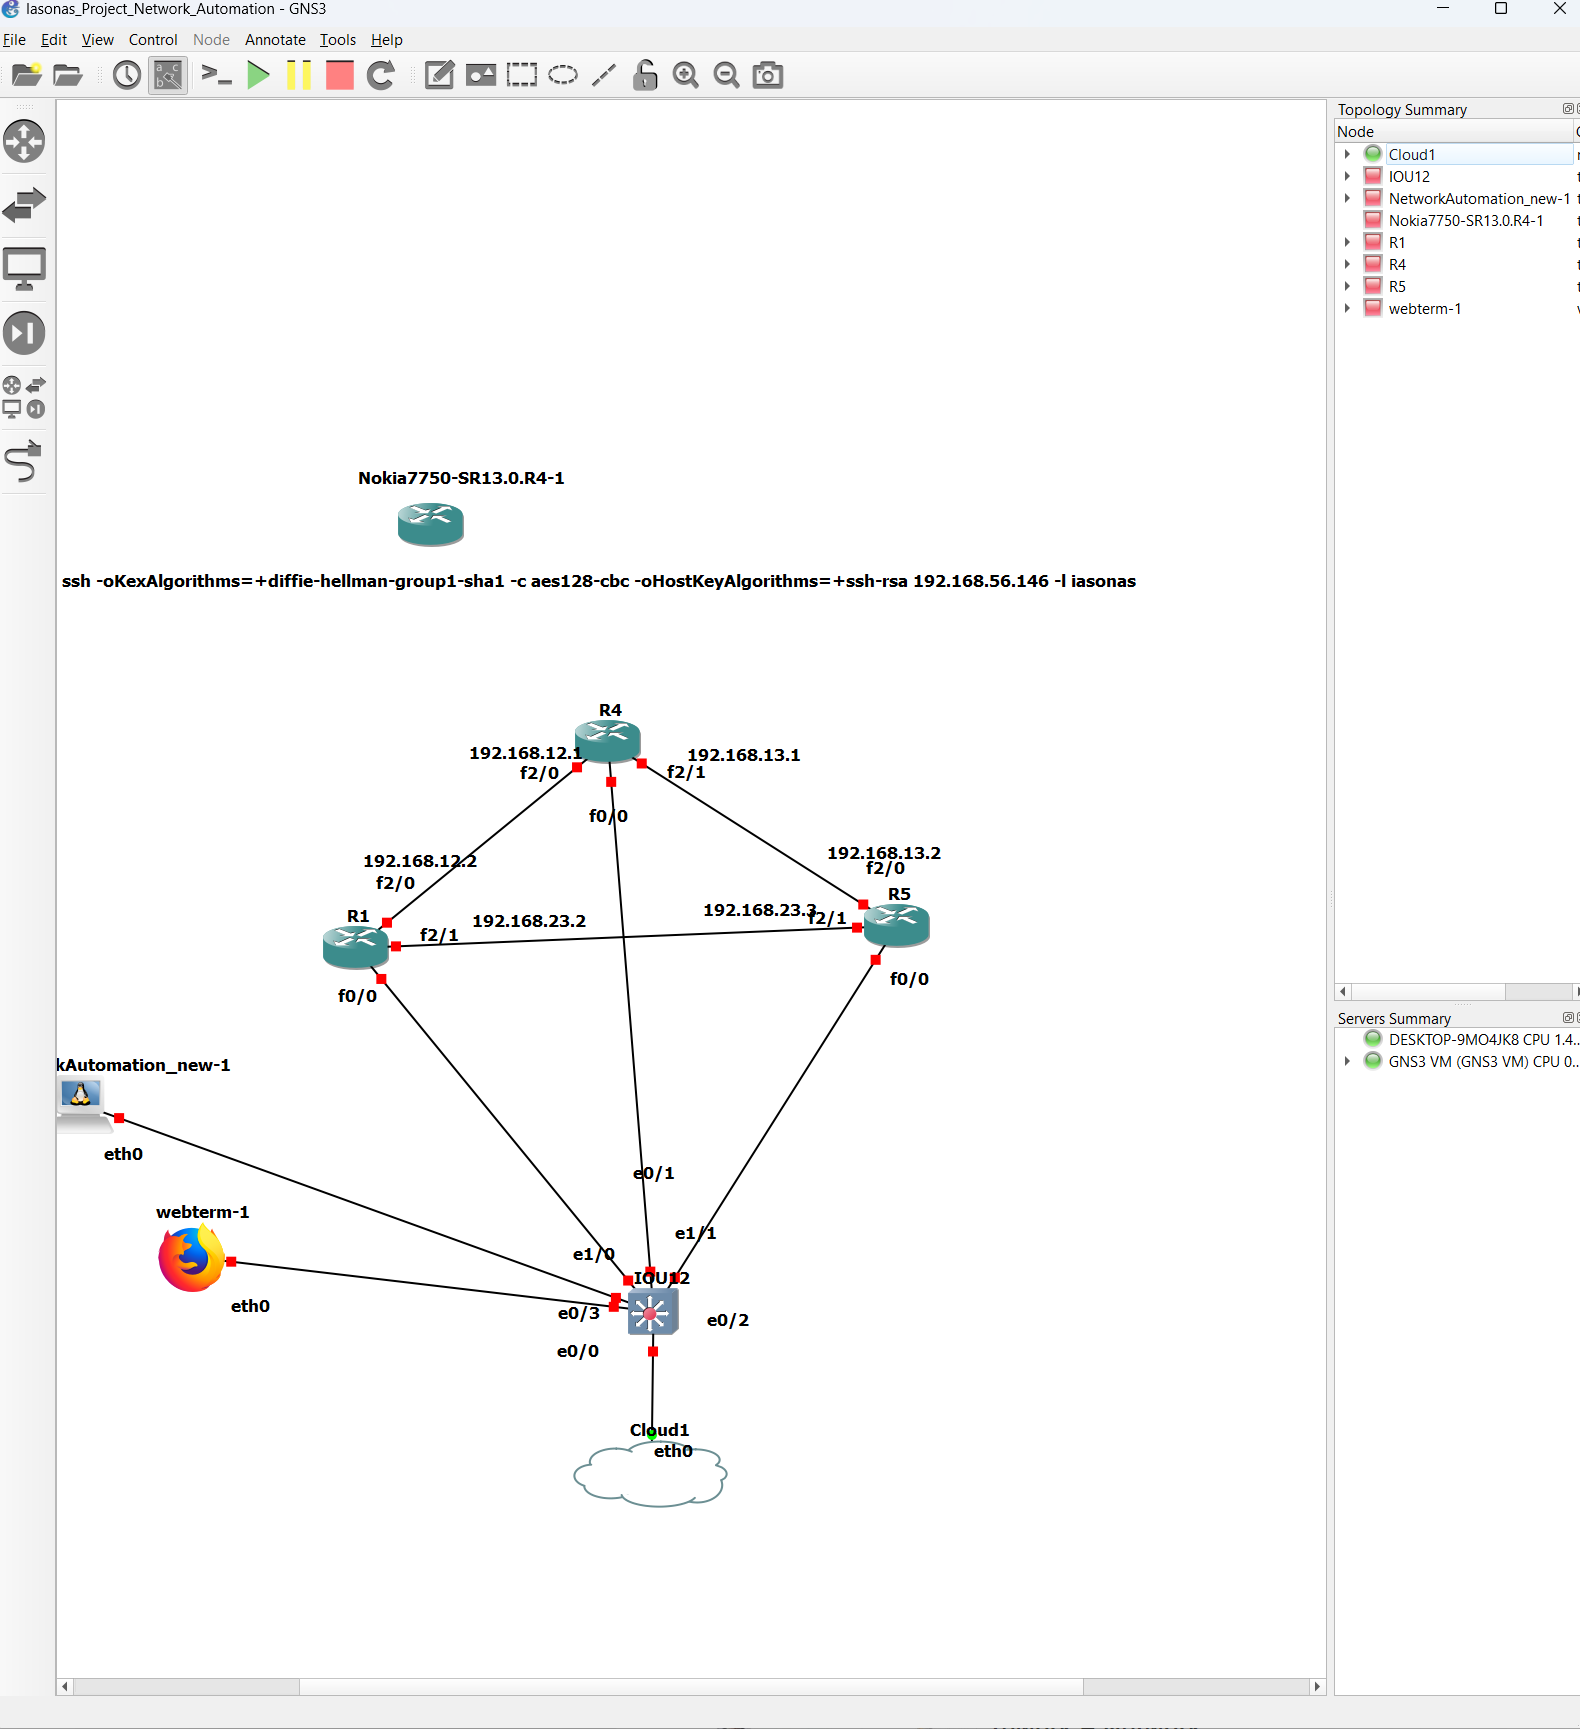
\includegraphics[width=0.7\textwidth]{graphics/gns3_homepage.png}
	\caption{\en{GNS3 homepage} }
\end{figure}

Προκειμένου να μπορέσει να επικοινωνήσει το \en{PC} μας στο τοπικό δίκτυο με το \en{GNS3 VM} στο τοπικό δίκτυο
θα πρέπει να γίνουν κάποιες ρυθμίσεις τόσο στο \en{GNS3 VM} όσο και στις συσκευές της \en{Cisco}

Στις συσκευές της \en{Cisco} θα πρέπει να γίνει η παρακάτω παραμετροποίηση όπως εμφανίζεται στις εικόνες 4.1,4.2,4.3.

\begin{figure}[htb]
	\centering
	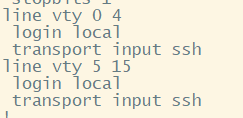
\includegraphics[width=0.7\textwidth]{graphics/cisco_ssh_config.png}
	\caption{\en{Cisco ssh config} }
\end{figure}

\begin{figure}[htb]
	\centering
	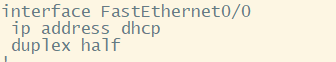
\includegraphics[width=0.7\textwidth]{graphics/dhcp_cisco_config.png}
	\caption{\en{Cisco dhcp config} }
\end{figure}


Μέχρι αυτή τη στιγμή έχουμε παραμετροποιήσει τις συσκευές με τέτοιο τρόπο ώστε να δέχονται
απομακρυσμένη σύνδεση. Τώρα θα εξηγήσουμε πως μπορούμε να φτιάξουμε την εποικοινωνία μεταξύ εικονικών
μηχανών της \en{Cisco} και του τοπικού μας υπολογιστή. Η λογική είναι ότι η συσκευή \en{Cloud}
θα μας επιτρέψει να φτιάξουμε τη σύνδεση αυτή. Η εικόνα 4.4 μας παρουσιάζει σε ανώτερο επίπεδο τη λογική αυτή σύνδεση.

\begin{figure}[htb]
	\centering
	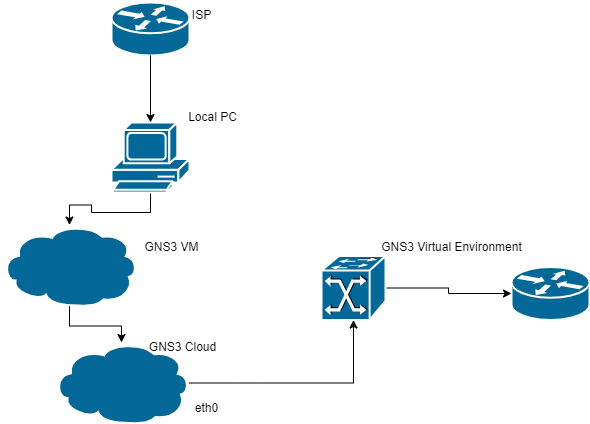
\includegraphics[width=0.7\textwidth]{graphics/diagram.drawio.png}
	\caption{\en{Local PC-GNS3VM-CISCO IOS Connection Architecture} }
\end{figure}









\section{\en{Connection Establishment} }


Μετά την ολοκλήρωση της παραμετροποίησης και της διαμόρφωσης της τοπολογίας, όλα τα διαφορετικά στοιχεία (\en{components}) 
θα πρέπει να ανήκουν στο ίδιο τοπικό δίκτυο. Η εικονική διεπαφή μέσω της οποίας θα διέρχεται όλη η δικτυακή κίνηση, είτε πρόκειται για \en{REST}
είτε για \en{SSH}, είναι η διεπαφή \en{eth0} στο περιβάλλον του \en{GNS3 VM}. Στην εικόνα 4.6 παρατίθεται ένα αρχείο καταγραφής (\en{trace}), 
το οποίο επιβεβαιώνει ότι η σύνδεση πραγματοποιείται απρόσκοπτα.

Η βασική απαίτηση είναι η διεπαφή μεταξύ του \en{GNS3 VM} και του τοπικού υπολογιστή να ανήκουν στο ίδιο δίκτυο. 
Για να επιτευχθεί αυτό, εφαρμόστηκε η κατάλληλη παραμετροποίηση στο \en{GNS3 VM}, όπως παρουσιάζεται στο Σχήμα 4.5. 
Με αυτόν τον τρόπο, εφόσον το \en{GNS3 VM} έχει ενταχθεί στο τοπικό δίκτυο, το ίδιο μπορεί να συμβεί και για τις συσκευές της \en{Cisco}
, οι οποίες θα εισαχθούν στο περιβάλλον εργασίας μας, επιτρέποντας τη διαδραστικότητα και την επικοινωνία με αυτές.

\begin{figure}[htb]
	\centering
	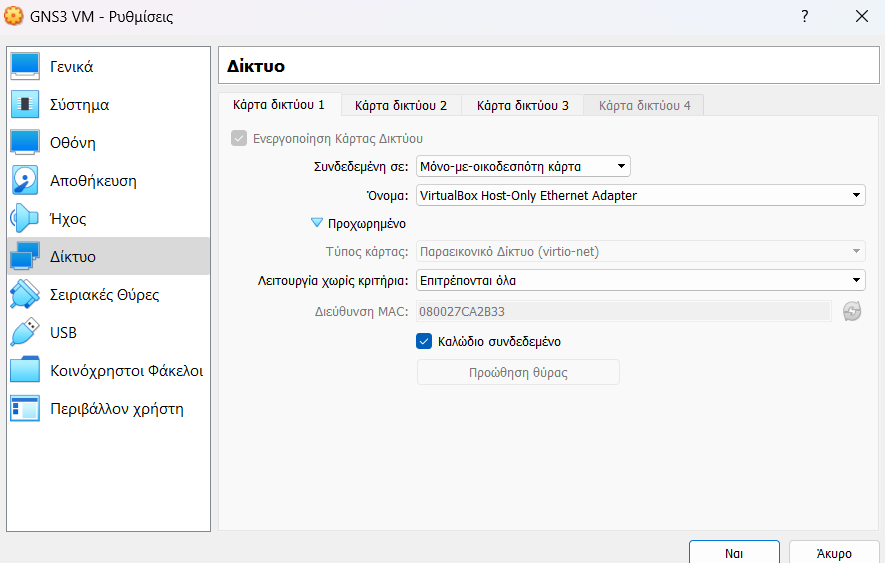
\includegraphics[width=1.0\textwidth]{graphics/network_config_GNS3.png}
	\caption{\en{Network Configuration for GNS3VM} }
\end{figure}


\begin{figure}[htb]
	\centering
	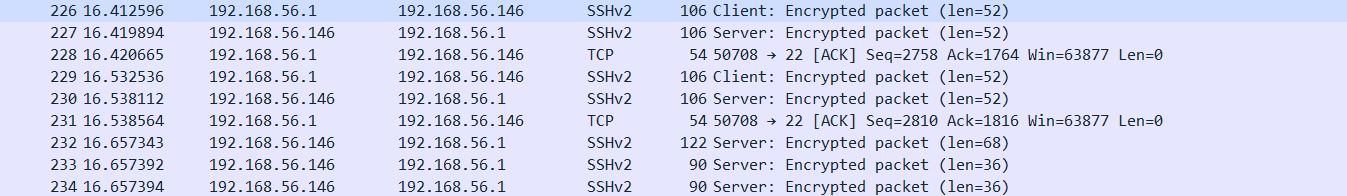
\includegraphics[width=1.0\textwidth]{graphics/ssh_connection.png}
	\caption{\en{SSH traffic} }
\end{figure}


Προκειμένου να γίνει η συλλογή του συγκεκριμένου \en{trace} χρησιμοποιήθηκε η παρακάτω εντολή:
\en{ tcpdump -i eth0 -v -w /home/gns3/test.pcap}
.Η συλλογή του \en{trace} έγινε με το πρωτόκολλο \en{SFTP}.


\begin{figure}[h]
	\centering
	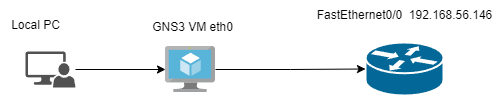
\includegraphics[width=0.7\textwidth]{graphics/jason1.png}
	\caption{\en{SSH traffic} }
\end{figure}

\FloatBarrier

\section{Σύνδεση με \en{Django Server} }

Ο \en{Django Server} τρέχει στον τοπικό υπολογιστή. Μπορεί να τρέξει σε οποιοδήποτε
μηχάνημα είναι \en{Linux} είτε \en{Windows} αρκεί να είναι στο τοπικό δίκτυο
είτε να υπάρχει κάποια συσκευή \en{layer2} η οποία να αναλάβει τη σύνδεση στο λεγόμενο
\en{data link layer}.


\section{Δομή της διαδικτυακής εφαρμογής \en{Django} }


\subsection{Τα αρχεία \en{urls.py}}
Τα αρχεία αυτά καθορίζουν τη δρομολόγηση των \en{URL} της εφαρμογής. 
Οι διευθύνσεις \en{URL} που αντιστοιχούν στα μοτίβα που περιγράφονται στο αρχείο \en{urls.py} 
προωθούνται στην αντίστοιχη συνάρτηση στο αρχείο \en{views.py}. 
Η αντιστοίχιση πραγματοποιείται σειριακά από πάνω προς τα κάτω στο αρχείο \en{urls.py}. 
Παρόλο που σε αυτό το έργο υλοποιήθηκε ακριβής αντιστοίχιση των \en{URL}, το \en{Django} παρέχει τη 
δυνατότητα χρήσης ταυτοποίησης μέσω κανονικών εκφράσεων. Στην εικόνα που ακολουθεί, παρουσιάζονται οι 
διευθύνσεις \en{URL} του \en{API}, όπου κάθε διεύθυνση αντιστοιχεί σε μια συνάρτηση στο αρχείο \en{api1/views.py}, 
η οποία καταλήγει στην εκτέλεση του αντίστοιχου σεναρίου

\begin{figure}[htb]
	\centering
	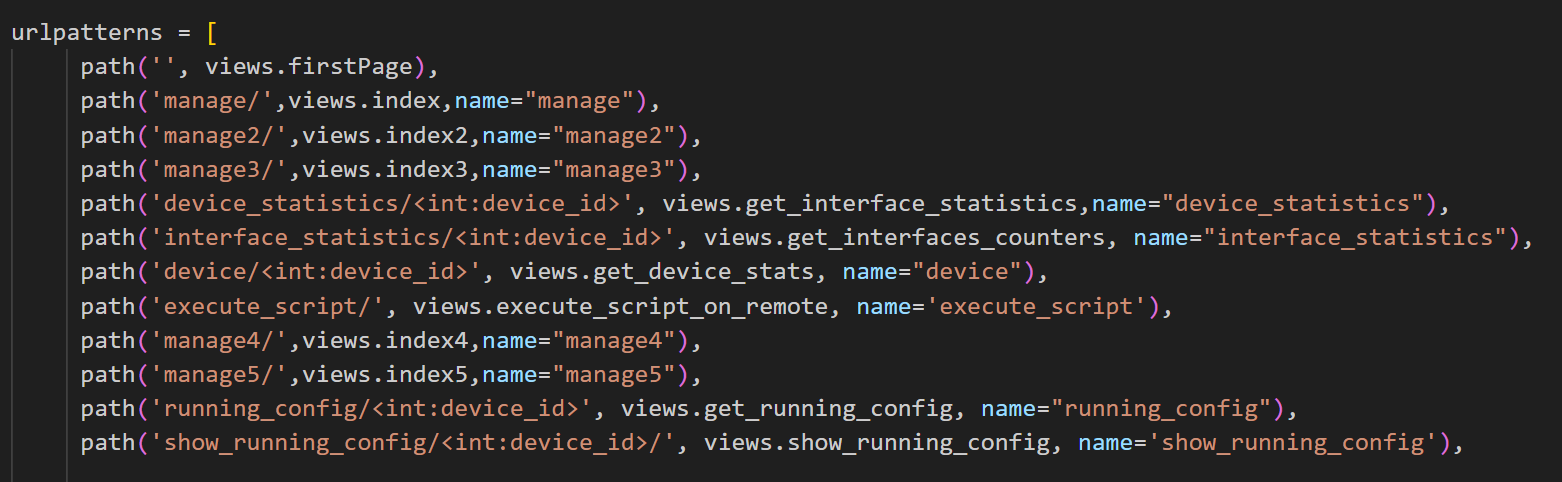
\includegraphics[width=0.9\textwidth]{graphics/urlpy.png}
	\caption{\en{url.py} }
\end{figure}

\subsection{Τα αρχεία \en{views.py}}

Οι συναρτήσεις σε ένα αρχείο \en{views.py} καλούνται όταν η δεδομένη διεύθυνση \en{URL} που αποστέλλεται από το
χρήστη ταιριάζει με το αντίστοιχο μοτίβο \en{URL} στο αρχείο \en{urls.py}. Παράμετροι που αποστέλλονται μέσω κλήσης
\en{HTTP} εισέρχονται στην αντίστοιχη συνάρτηση μέσω παραμέτρων ή σώματος αίτησης. Στο αρχείο \en{views.py} του \en{API}, η συνάρτηση εκτελεί το σενάριο
κώδικα με τις δεδομένες παραμέτρους εισόδου. Όταν τελειώσει η εκτέλεση του κώδικα δέσμης ενεργειών,
το αποτέλεσμα επιστρέφεται στη συνάρτηση \en{views} και μεταβιβάζεται ως πλαίσιο στο αντίστοιχο αρχείο \en{.html} για την εμφάνιση των αποτελεσμάτων στον χρήστη που εκτέλεσε το σενάριο.
Ένα παράδειγμα μιας συνάρτησης σε ένα αρχείο en{views.py} μπορείτε να δείτε στο σχήμα παρακάτω

\begin{figure}[htb]
	\centering
	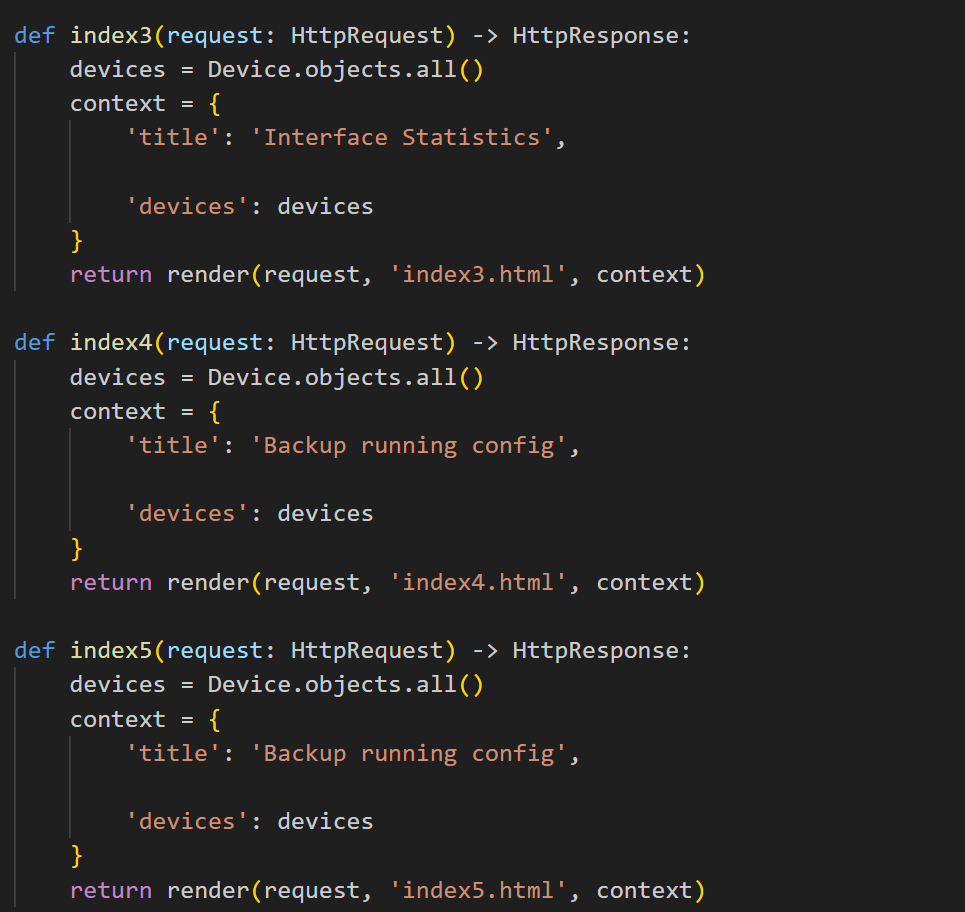
\includegraphics[width=0.9\textwidth]{graphics/viewspy.png}
	\caption{\en{views.py} }
\end{figure}

\subsection{Τα αρχεία \en{html template}}

Στη συνάρτηση \en{views.py}, το \en{Django} αποδίδει το αντίστοιχο πρότυπο \en{.html}
αρχείο με ένα συγκεκριμένο πλαίσιο. Το πλαίσιο είναι σε μορφή \en{JavaScript Object Notation (JSON)} και αποστέλλεται στο αρχείο \en{.html}. Τα δεδομένα στο πλαίσιο εμφανίζονται
στο \en{.html}, εάν το \en{.html} έχει παραμετροποιηθεί κατάλληλα. Ένα παράδειγμα \en{.html} με
τον συντακτικό κώδικα για τον τρόπο πρόσβασης στα δεδομένα του πλαισίου παρουσιάζεται στην εικόνα παρακάτω



\begin{figure}[htb]
	\centering
	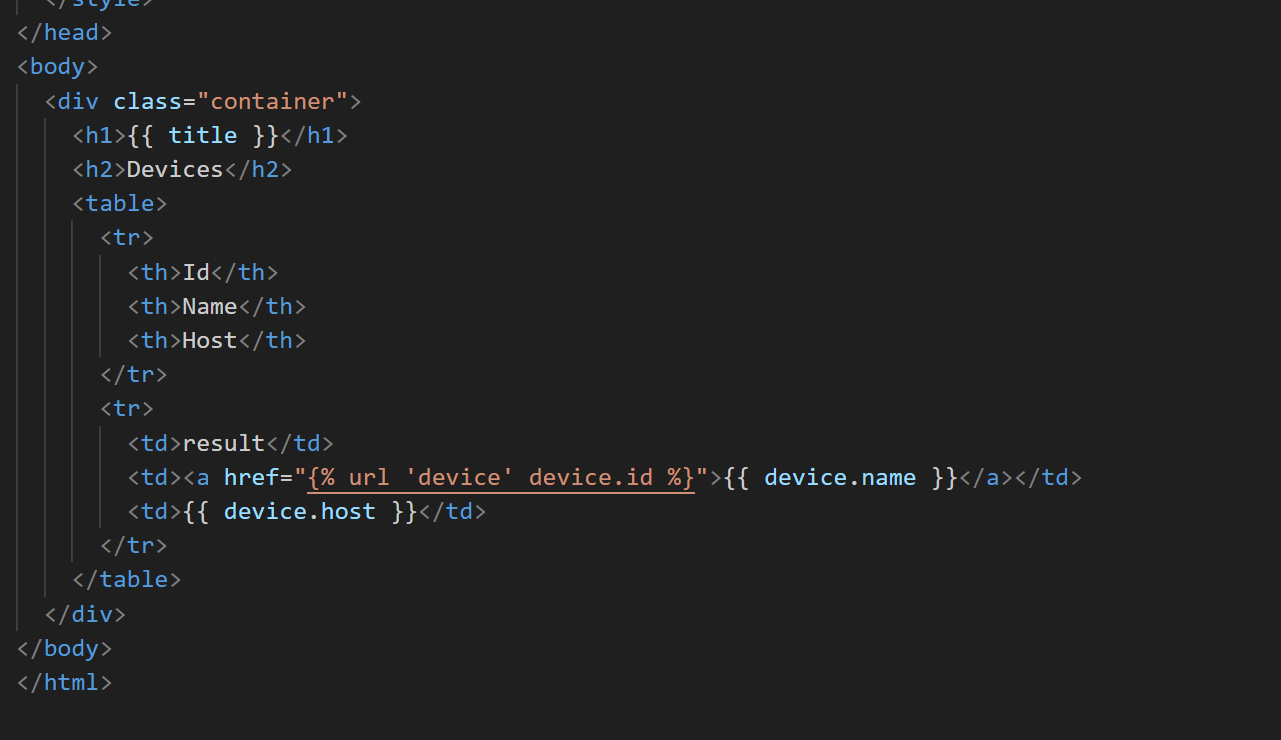
\includegraphics[width=0.9\textwidth]{graphics/html_template.png}
	\caption{Παράδειγμα \en{html} αρχείου }
\end{figure}






\subsection{Η βάση δεδομένων}
Η διαδικτυακή πύλη χρησιμοποιεί μια βάση δεδομένων \en{SQLite}. Αυτή η βάση δεδομένων περιέχει τρία
μοντέλα τα οποία ορίζονται στο αρχείο \en{models.py}. Το αρχείο αυτό περιέχει μία κλαση Device η οποία δέχεται σαν ορίσματα
το όνομα, την \en{IP}, το όνομα χρήστη, τον κωδικό, τον κρυφό κωδικό και το μοντέλο της συσκευής.
Υπάρχει μία εγγραφή στη βάση δεδομένων ένα από αυτά τα αντικέιμενα τα οποία εμείς τα δημιουργούμε. Το μοντέλο διαπιστευτηρίων αποθηκεύει τα διαπιστευτήρια τα οποία έχουν προηγουμένως
κρυπτογραφημένα. Με αυτό, ορισμένες δέσμες ενεργειών μπορούν να λάβουν τα διαπιστευτήρια που απαιτούνται για να λειτουργήσουν
χωρίς την είσοδο του χρήστη και χωρίς να γίνεται άμεση αναφορά στα διαπιστευτήρια στο
κώδικα.
Η διαχείριση της βάσης δεδομένων μπορεί να γίνει απευθείας μέσω μιας γραφικής διεπαφής χρήστη
\en{(GUI)} στο \en{Django}. Σε αυτό το \en{GUI} μπορούν να έχουν πρόσβαση μόνο οι χρήστες διαχειριστές. Παραδείγματα
των εγγραφών του μοντέλου της εφαρμογής  που εμφανίζονται σε αυτό το \en{GUI} παρουσιάζονται παρακάτω στην εικόνα.

\begin{figure}[htb]
	\centering
	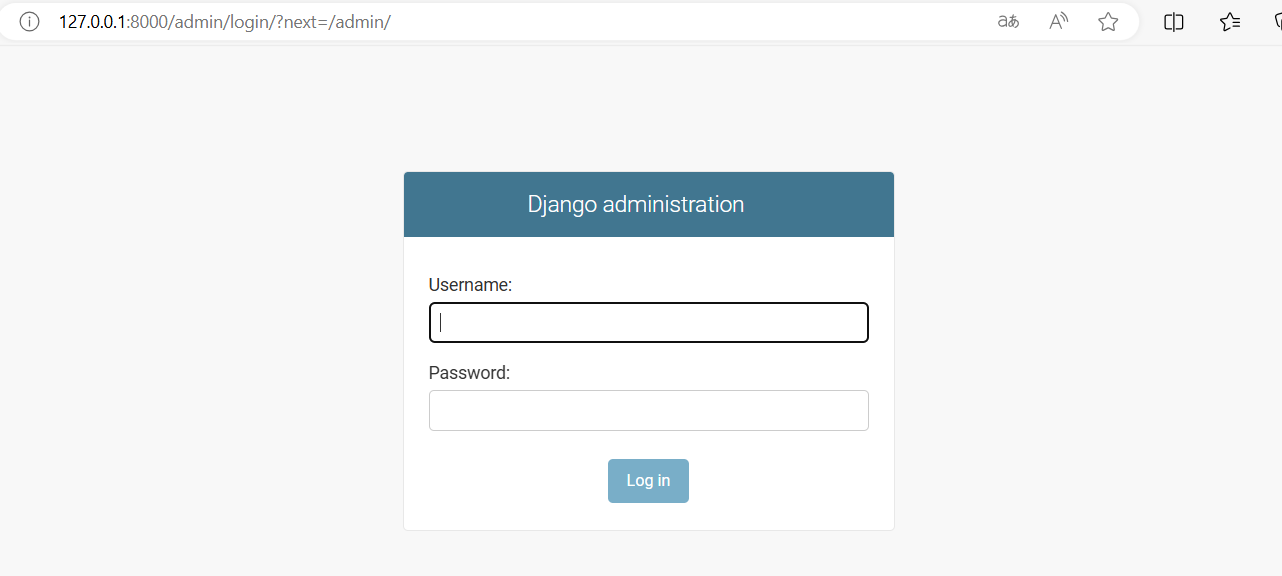
\includegraphics[width=0.9\textwidth]{graphics/GUI_LOGIN.png}
	\caption{Είσοδος στο \en{GUI}}
\end{figure}

\begin{figure}[htb]
	\centering
	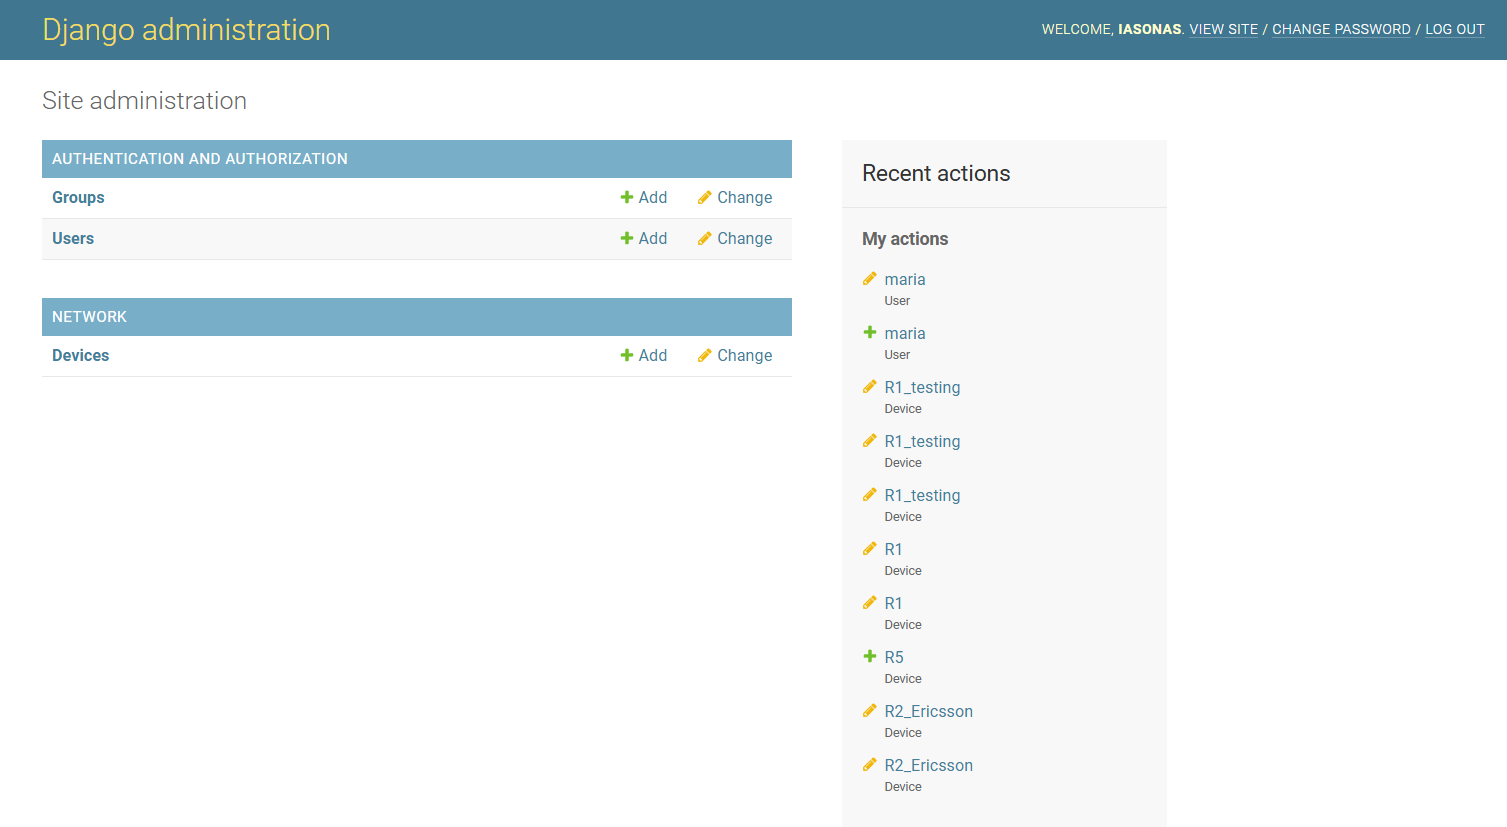
\includegraphics[width=0.9\textwidth]{graphics/DJANGO_ADMIN.png}
	\caption{Κεντρική σελίδα του \en{Django Administration GUI}}
\end{figure}

\begin{figure}[htb]
	\centering
	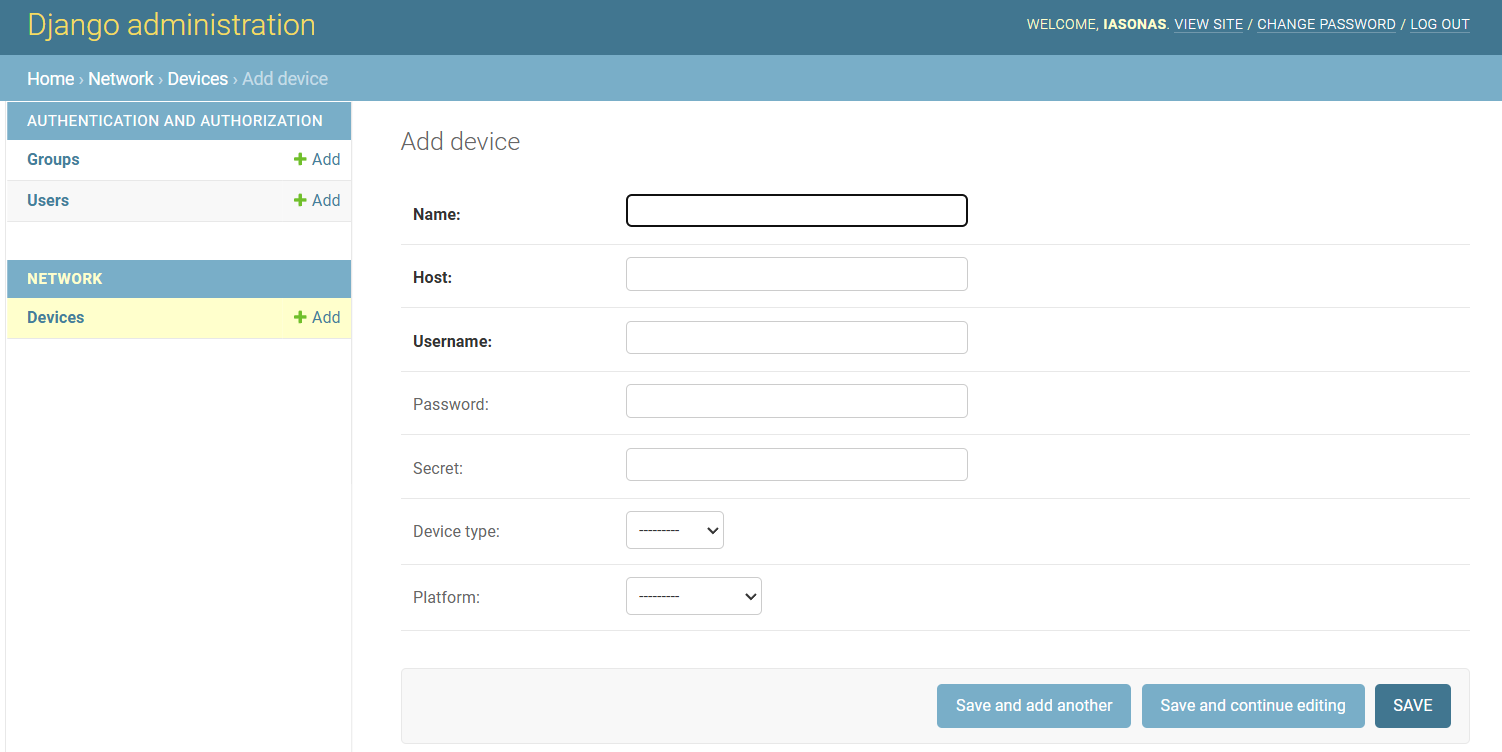
\includegraphics[width=0.9\textwidth]{graphics/ADD_DEVICE.png}
	\caption{Προσθήκη συσκευής }
\end{figure}


 Η προσθήκη συσκευής γίνεται συμπληρώνοντας στοιχεία όπως η \en{IP} διεύθυνση, το \en{username}, το \en{password} ,\en{secret} και το όνομα. Αν δώσουμε αυτά τα στοιχεία
 μετά το λογισμικό θα μπορέσει να κάνει τη δουλειά προκειμένου να μπει στη συσκευή και να εκτελέσει βασικές λειτουργίες που θα παρουσιάσουμε και παρακάτω. 







 

\chapter{Υλοποίηση της εφαρμογης}

%Το \en{Lorem Ipsum} είναι απλά ένα κείμενο χωρίς νόημα για τους επαγγελματίες της τυπογραφίας και στοιχειοθεσίας \cite{LoremIpsumAll}. Το \en{Lorem Ipsum} είναι το επαγγελματικό πρότυπο όσον αφορά το κείμενο χωρίς νόημα, από τον 15ο αιώνα, όταν ένας ανώνυμος τυπογράφος πήρε ένα δοκίμιο και ανακάτεψε τις λέξεις για να δημιουργήσει ένα δείγμα βιβλίου. Όχι μόνο επιβίωσε πέντε αιώνες, αλλά κυριάρχησε στην ηλεκτρονική στοιχειοθεσία, παραμένοντας με κάθε τρόπο αναλλοίωτο. Έγινε δημοφιλές τη δεκαετία του '60 με την έκδοση των δειγμάτων της \en{Letraset} όπου περιελάμβαναν αποσπάσματα του \en{Lorem Ipsum}, και πιο πρόσφατα με το λογισμικό ηλεκτρονικής σελιδοποίησης όπως το \en{Aldus PageMaker} που περιείχαν εκδοχές του \en{Lorem Ipsum}.
\section{Ανάπτυξη με το  \en{Django framework}}

\subsection{Δημιουργία \en{Models}}

Η διαδικτυακή πύλη χρησιμοποιεί μια βάση δεδομένων \en{SQLite}. Αυτή η βάση δεδομένων περιέχει τρία
μοντέλα τα οποία ορίζονται στο αρχείο \en{models.py}. Στην εικόνα 6.1 φαίνονται τα μοντέλα αυτά.

\FloatBarrier

\begin{figure}[htb]
	\centering
	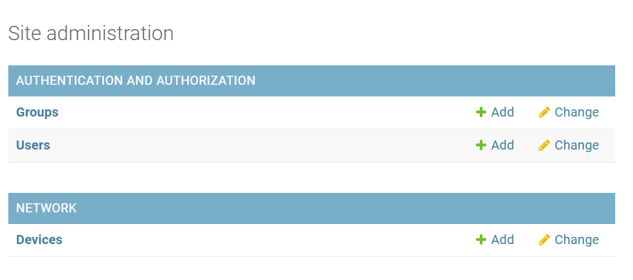
\includegraphics[width=0.9\textwidth]{graphics/models_2.png}
	\caption{Μοντέλα}
\end{figure}

\FloatBarrier


Η διαδικτυακή πύλη περιέχει την κλάση \en{Device}, η οποία δέχεται ως ορίσματα το όνομα, τη διεύθυνση \en{IP}, το όνομα χρήστη, τον κωδικό πρόσβασης, τον κρυφό κωδικό και το μοντέλο της συσκευής. Για κάθε μία από αυτές τις συσκευές που δημιουργούμε, καταγράφεται μια αντίστοιχη εγγραφή στη βάση δεδομένων. Το αντικείμενο που δημιουργείται δηλαδή η συσκευή προς δοκιμή περιλαμβάνει πεδία που αξιοποιούνται από τις συναρτήσεις του αρχείου \en{views.py}. Με αυτόν τον τρόπο, τα πεδία του αντικειμένου αποθηκεύονται και χρησιμοποιούνται ως ορίσματα μέσα στις συναρτήσεις, διευκολύνοντας τη διαχείριση και την επεξεργασία των δεδομένων της συσκευής




\subsection{\en{Views} και \en{Urls}}


 Τα αρχεία \en{Urls} καθορίζουν τη δρομολόγηση των \en{URL} της εφαρμογής. Οι διευθύνσεις \en{URL} που αντιστοιχούν στα μοτίβα που περιγράφονται στο αρχείο \en{urls.py} προωθούνται στην αντίστοιχη συνάρτηση στο αρχείο \en{views.py}. Η αντιστοίχιση πραγματοποιείται σειριακά από πάνω προς τα κάτω στο αρχείο \en{urls.py} όπως φαίνεται στη εικόνα 6.2. 

\FloatBarrier

\begin{figure}[htb]
	\centering
	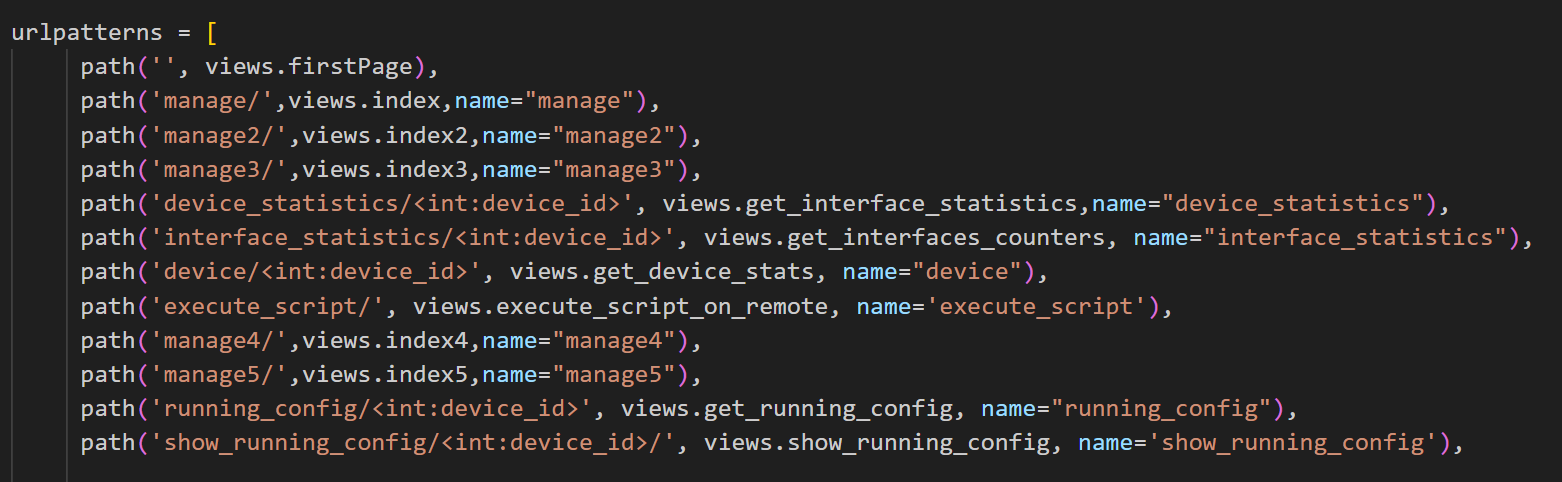
\includegraphics[width=0.9\textwidth]{graphics/urlpy.png}
	\caption{\en{urls.py} }
\end{figure}

\FloatBarrier

Παρόλο που σε αυτό το έργο υλοποιήθηκε ακριβής αντιστοίχιση των \en{URL}, το \en{Django} παρέχει τη 
δυνατότητα χρήσης ταυτοποίησης μέσω κανονικών εκφράσεων. Στην εικόνα που ακολουθεί, παρουσιάζονται οι 
διευθύνσεις \en{URL} του \en{API}, όπου κάθε διεύθυνση αντιστοιχεί σε μια συνάρτηση στο αρχείο \en{api1/views.py}, 
η οποία καταλήγει στην εκτέλεση του αντίστοιχου σεναρίου



Οι συναρτήσεις σε ένα αρχείο \en{views.py} καλούνται όταν η δεδομένη διεύθυνση \en{URL} που αποστέλλεται από το
χρήστη ταιριάζει με το αντίστοιχο μοτίβο \en{URL} στο αρχείο \en{urls.py}. Παράμετροι που αποστέλλονται μέσω κλήσης
\en{HTTP} εισέρχονται στην αντίστοιχη συνάρτηση μέσω παραμέτρων ή σώματος αίτησης. Στο αρχείο \en{views.py} του \en{API}, η συνάρτηση εκτελεί το σενάριο
κώδικα με τις δεδομένες παραμέτρους εισόδου. Όταν τελειώσει η εκτέλεση του κώδικα δέσμης ενεργειών,
το αποτέλεσμα επιστρέφεται στη συνάρτηση \en{views} και μεταβιβάζεται ως πλαίσιο στο αντίστοιχο αρχείο \en{.html} για την εμφάνιση των αποτελεσμάτων στον χρήστη που εκτέλεσε το σενάριο.
Ένα παράδειγμα τριών διαφορετικών συνάρτησεων σε ένα αρχείο \en{views.py} μπορείτε να δείτε στο σχήμα 6.3.

\FloatBarrier

\begin{figure}[htb]
	\centering
	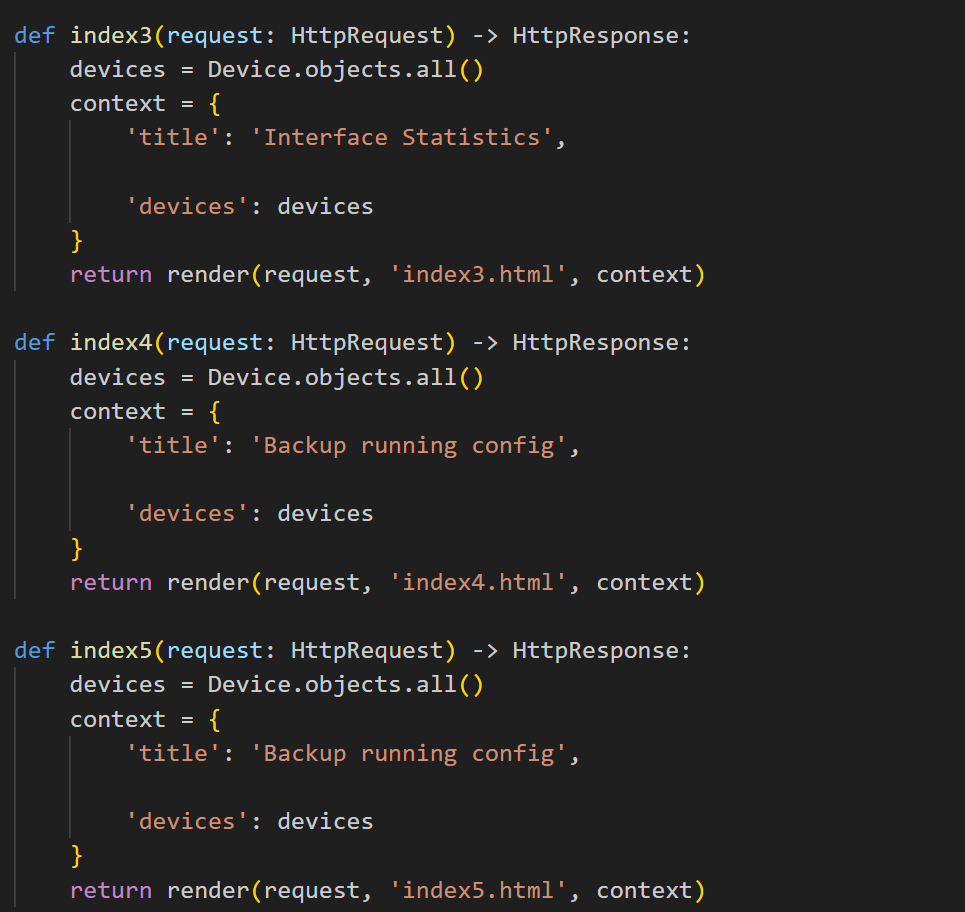
\includegraphics[width=0.9\textwidth]{graphics/viewspy.png}
	\caption{\en{views.py} }
\end{figure}

\FloatBarrier

\subsection{\en{User Interface (Templates)}}


Σε κάθε συνάρτηση του αρχείου \en{views.py}, το \en{Django} αποδίδει το αντίστοιχο πρότυπο \en{.html}
αρχείο με ένα συγκεκριμένο πλαίσιο. Η λογική είναι ότι κάθε \en{HTTP Request} που δέχεται όταν ο χρήστης επιδρά με την εφαρμογή απαντιέται με ένα αντίστοιχο \en{HTTP Response} . Τα δεδομένα στο πλαίσιο εμφανίζονται
στο \en{.html} μέσα από το \en{HTTP Response}, εάν το \en{.html} έχει παραμετροποιηθεί κατάλληλα. Ένα παράδειγμα \en{.html} με
τον συντακτικό κώδικα για τον τρόπο πρόσβασης στα δεδομένα του πλαισίου παρουσιάζεται στην εικόνα 6.4.

\FloatBarrier

\begin{figure}[htb]
	\centering
	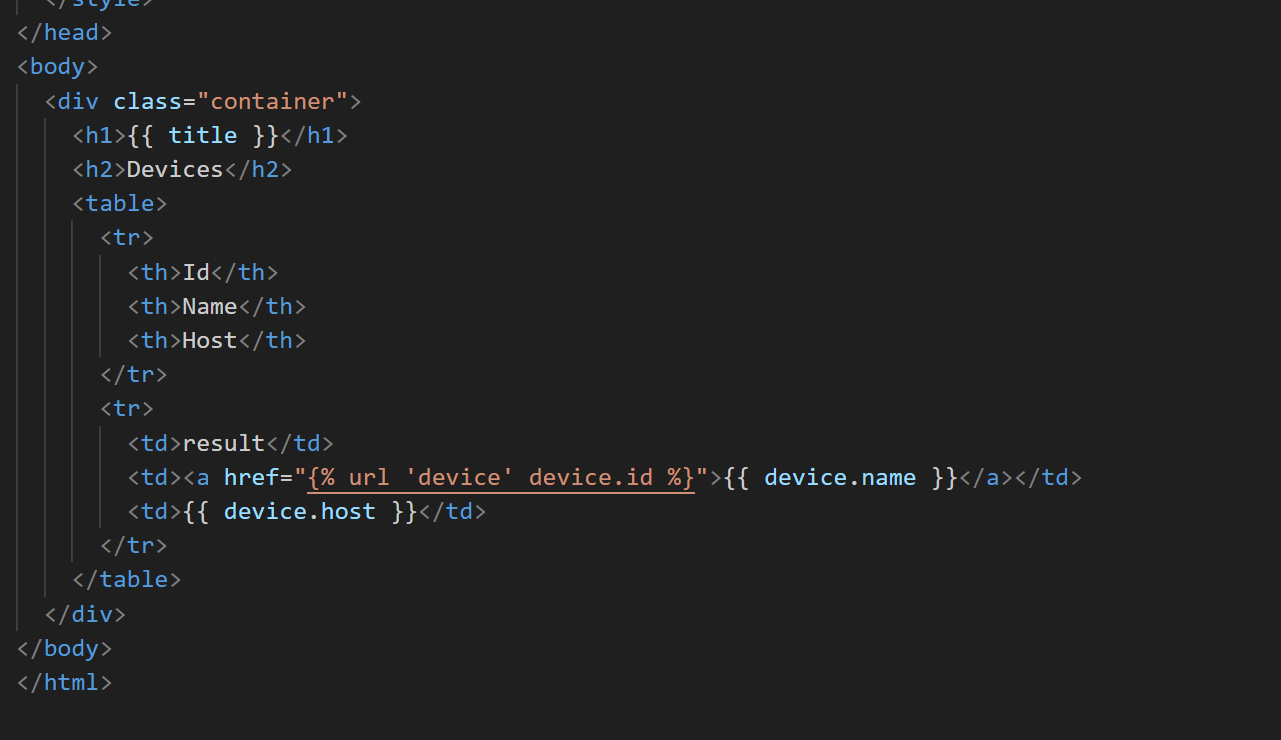
\includegraphics[width=0.9\textwidth]{graphics/html_template.png}
	\caption{Παράδειγμα \en{html} αρχείου }
\end{figure}

\FloatBarrier

Έτσι όλη η διαθέσιμη λειτουργικότητα που παρέχεται στον χρήστη της εφαρμογής διαχείρισης δικτύου υλοποιείται με την χρήση \en{URLs} (κλήσεις συναρτήσεων και \en{html} αρχείων). Έτσι για παράδειγμα για την λειτουργία \en{Statistics} : 

\begin{itemize}
    \item Ο χρήστης επισκέπτεται το \en{URL} \en{/manage3}. 
    \item Ο ορισμός του \en{URL} στο \en{urls.py} κατευθύνει το αίτημα στη συνάρτηση \en{index2} στο \en{views.py}.
    \item Με αυτό τον τρόπο ο χρήστης κάνει ένα \en{HTTP Request}. Η συνάρτηση \en{index2} συλλέγει τα δεδομένα (\en{context-data}) που χρειάζονται για την προβολή.
    \item Η συνάρτηση \en{index2} επιστρέφει τα δεδομένα στη σελίδα \en{index2.html} επιστρέφοντας το μέσα από ένα \en{HTTP Response}.
    \item Το \en{template} \en{index2.html} λαμβάνει τα δεδομένα και τα εμφανίζει στον χρήστη.
\end{itemize}


\section{\en{REST API Integration} και διασύνδεση με το \en{SSH protocol}}

 Το \en{REST API Integration} διαδραματίζει κρίσιμο ρόλο στη 
διπλωματική εργασία, καθώς επιτρέπει την αλληλεπίδραση μεταξύ των 
διαφόρων συστημάτων και την ανταλλαγή δεδομένων μέσω του διαδικτύου. 
Το \en{REST} (\en{Representational State Transfer}) είναι μια 
αρχιτεκτονική προσέγγιση που χρησιμοποιεί τα πρωτόκολλα \en{HTTP} 
για την εκτέλεση λειτουργιών όπως η ανάκτηση, η δημιουργία, η 
ενημέρωση και η διαγραφή δεδομένων. Με την υλοποίηση \en{REST APIs}, 
καθίσταται δυνατή η διαλειτουργικότητα της εφαρμογής με άλλες 
υπηρεσίες, διευκολύνοντας τη σύνθεση πολύπλοκων λειτουργιών από 
διάφορες πηγές. Στο πλαίσιο της διπλωματικής, το \en{REST API} 
χρησιμοποιείται για την διαχείριση δικτυακών συσκευών, παρακολούθηση 
στατιστικών, εκτέλεση εντολών, διασφαλίζοντας την ασφάλεια και την 
αποδοτικότητα της επικοινωνίας μέσω διαφανών και επεκτάσιμων 
τεχνολογιών. Το \en{REST} δεν χρησιμοποιείται για την επικοινωνία της εφαρμογής
και των συσκευών αλλά εσωτερικά ως μηχανισμός δρομολόγησης προκειμένου η εφαρμογή
να μπορεί να φέρει στον χρήστη το σωστό αποτέλεσμα. Η διαχείρηση των δικτυακών
συσκευών γίνεται με το πρωτόκολλο \en{SSH}.

Προσπαθώντας μέσα από το \en{wireshark} να πιάσουμε την κίνηση μεταξύ
\en{WSL} και δικτυακής συσκευής κάναμε το παρακάτω πείραμα προκειμένου να κατανοήσουμε 
πως επικοινωνεί η εφαρμογή με τις συσκευές. Πατάμε το κουμπί \en{R1 Testing} όπως φαίνεται στο σχήμα 6.5. και στο \en{Wireshark} κάνουμε \en{capture}
το \en{interface eth0} του \en{WSL} προκειμένου να δούμε τι γίνεται όταν εμείς πατάμε
το κουμπί για μια λειτουργία. Τα κουμπιά έχουν σχεδιαστεί έτσι ώστε, με το πάτημά τους, να σε κατευθύνουν μέσω συνδέσμου (\en{link}) στη λειτουργία που επιθυμείς να εκτελέσεις.


\FloatBarrier

\begin{figure}[htb]
	\centering
	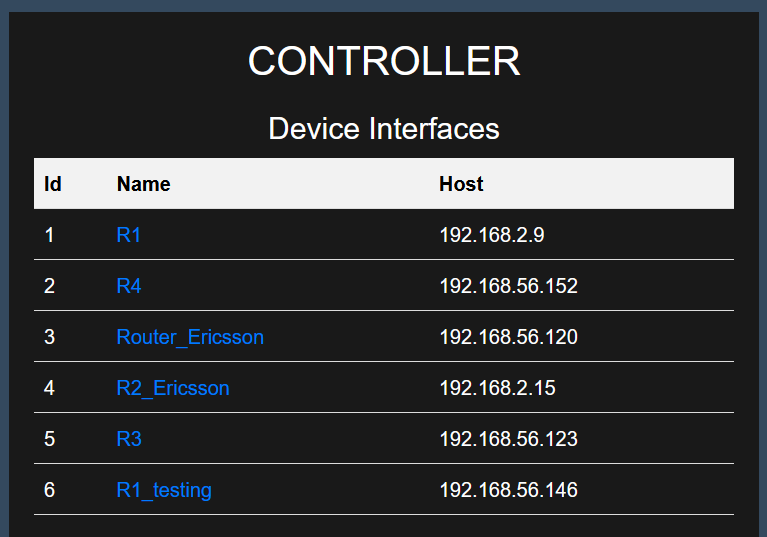
\includegraphics[width=0.9\textwidth]{graphics/r1_testing.png}
	\caption{Παράδειγμα \en{wireshark} }
\end{figure}

\FloatBarrier




\begin{figure}[htb]
	\centering
	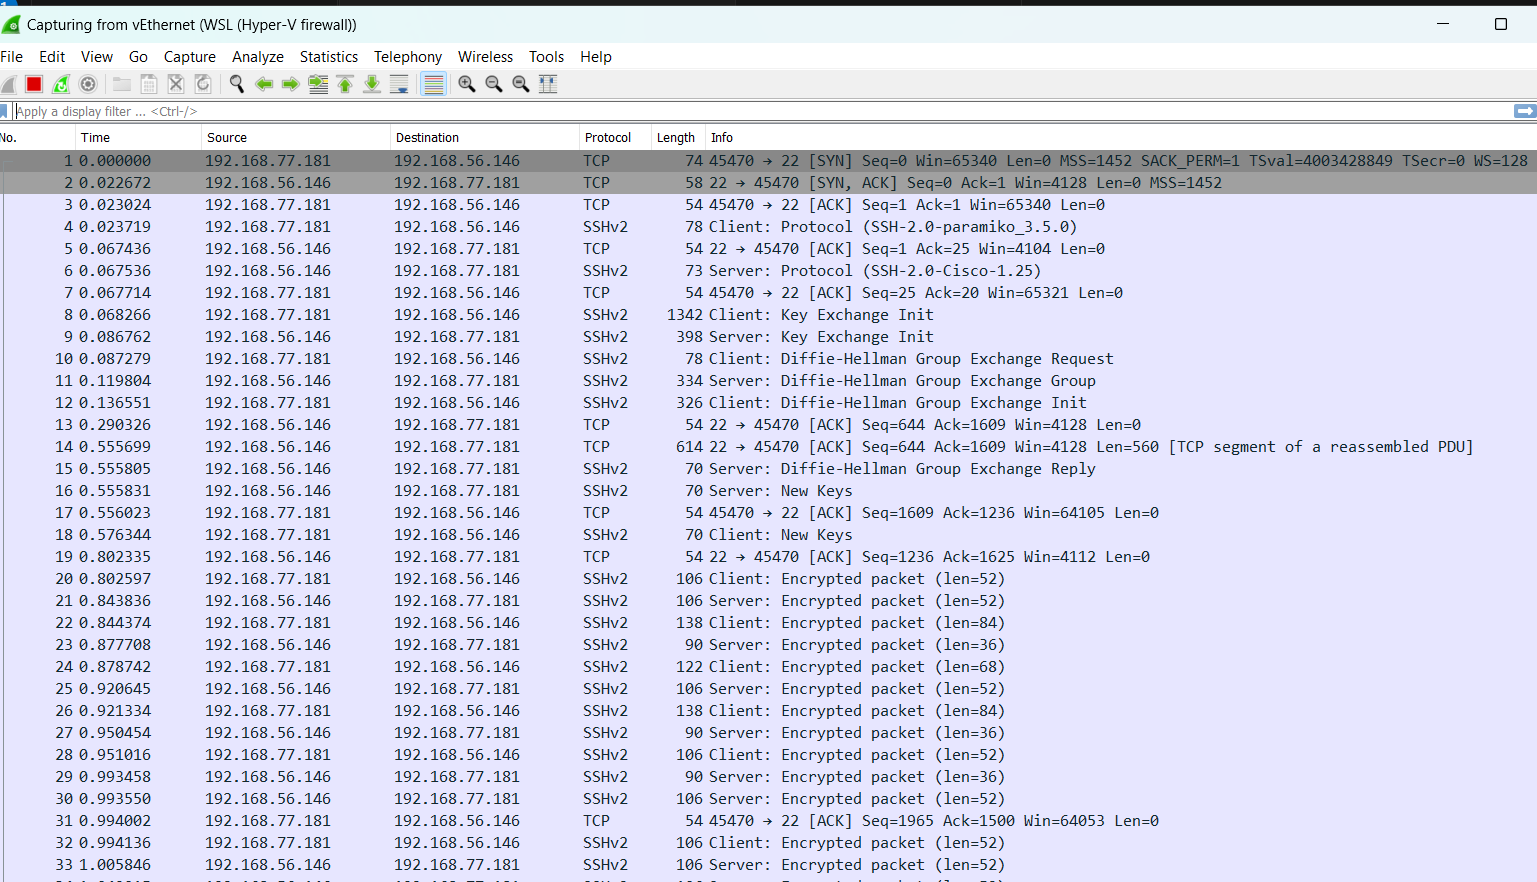
\includegraphics[width=0.9\textwidth]{graphics/wireshark.png}
	\caption{Παράδειγμα \en{wireshark} }
\end{figure}

\FloatBarrier

Αυτή η ακολουθία του σχήματος 6.6 αντιπροσωπεύει μια τυπική, ασφαλή σύνδεση \en{SSH}. Στο αρχείο \en{pcap} που καταγράψαμε, αποτυπώνεται η διαδικασία εγκαθίδρυσης μιας σύνδεσης \en{TCP} (\en{SYN, SYN/ACK, ACK}). Συγκεκριμένα, στο πρώτο πακέτο παρατηρούμε το \en{SYN}, το οποίο αποστέλλεται   προς τη συσκευή. Στη συνέχεια, η συσκευή αποκρίνεται με \en{SYN/ACK}, επιβεβαιώνοντας την επικοινωνία. Τέλος, στο τρίτο πακέτο, απαντάμε με \en{ACK}, ολοκληρώνοντας έτσι τη διαδικασία σύναψης της σύνδεσης.

Μετά ακολουθεί η διαπραγμάτευση πρωτοκόλλου \en{SSH} και στο τέλος η έναρξη της κρυπτογραφημένης επικοινωνίας την οποία δε μπορούμε να δούμε. Όμως μπορούμε να δούμε τι επιστρέφεται 
απο το \en{cli} του \en{Django server} στην  εικόνα 6.7.

\FloatBarrier
\begin{figure}[htb]
	\centering
	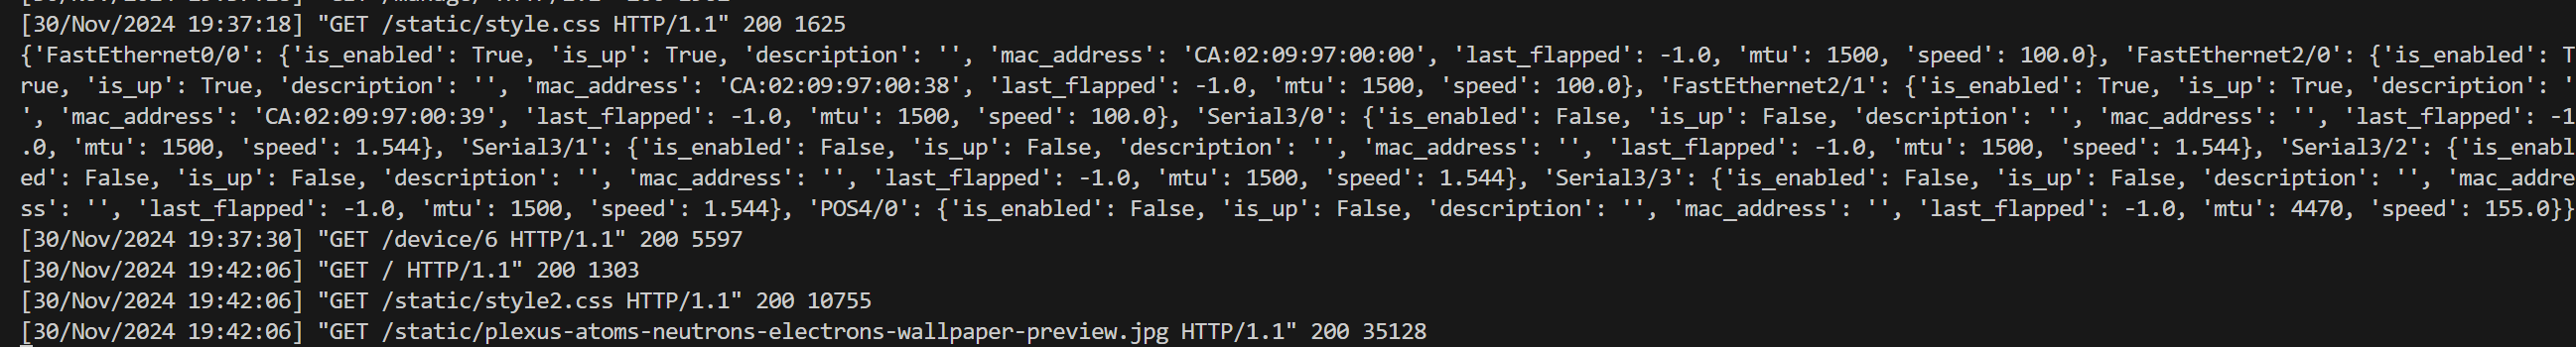
\includegraphics[width=0.9\textwidth]{graphics/rest.png}
	\caption{Απάντηση συσκευής}
\end{figure}

\FloatBarrier




%\begin{equation}
%	y = \alpha x + \beta
%\end{equation}

%Αντίθετα με αυτό που θεωρεί η πλειοψηφία, το \en{Lorem Ipsum} δεν είναι απλά ένα τυχαίο κείμενο. Οι ρίζες του βρίσκονται σε ένα κείμενο Λατινικής λογοτεχνίας του 45 π.Χ., φτάνοντας την ηλικία του πάνω από 2000 έτη.


%\begin{figure}[htb]
%	\centering
%	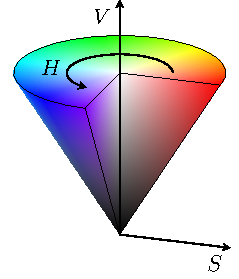
\includegraphics{tikz/hsv_cone/hsv_cone.pdf}
%	\caption{Ο χρωματικός χώρος \en{HSV}.}
%\end{figure}

\chapter{Επίδειξη της εφαρμογής(\en{Application Demo})}

\section{Εισαγωγή-Η λογική της λειτουργίας της εφαρμογής \en{Django}}

Όταν τρέχουμε τον διακομιστή της εφαρμογής η εφαρμογή ιστού
είναι διαθέσιμη από οποιοδήποτε φυλλομετρητή. Η αρχική σελίδα στη εφαρμογή
\en{Django} δηλώνεται στο πλαίσιο του \en{Django run server} ώς μία συνάρτηση της \en{Python}
η οποία δέχεται ένα \en{http request} και σαν απάντηση επιστρέφει την αρχική σελίδα(\en{index.html}).

Αυτό γίνεται μέσα από 2 κύριως μηχανισμούς.Η συνάρτηση \en{firstPage} ορίζεται στο αρχείο \en{views.py} της εφαρμογής. Παίρνει ως όρισμα ένα αντικείμενο \en{HttpRequest} 
(την αίτηση του χρήστη) και επιστρέφει ένα \en{HttpResponse} μέσω της render:

\begin{figure}[h]
	\centering
	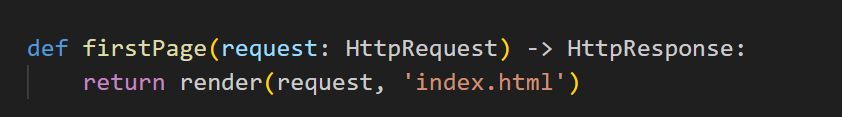
\includegraphics[width=1.0\textwidth]{graphics/firstPage.png}
	\caption{ \en{firstPage} συνάρτηση}
\end{figure}

Η λίστα \en{urlpatterns} συνδέει τη διεύθυνση \en{URL} 
με τη συνάρτηση \en{firstPage}. Το κενό \en{string} ('') σημαίνει ότι αυτή η διαδρομή αντιστοιχεί στη ρίζα του ιστότοπου (π.χ., \en{http://localhost:8000/})
Όταν ένας χρήστης επισκέπτεται τη ρίζα, η συνάρτηση \en{firstPage} 
εκτελείται και επιστρέφει την \en{HTML} σελίδα \en{index.html}. Παρακάτω το σημείο στο \en{urls.py} όπου γίνεται η δρομολόγηση.

\begin{figure}[h]
	\centering
	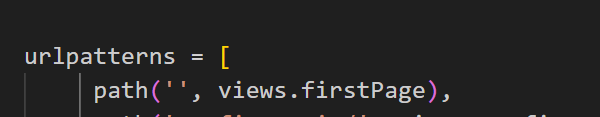
\includegraphics[width=1.0\textwidth]{graphics/urls_firstPage.png}
	\caption{ \en{Urls} δρομολόγηση για την αρχική σελίδα.}
\end{figure}


Μέσα από αυτή την αρχική σελίδα μπορούμε να κατευθυνθούμε σε οποιαδήποτε επιλογή εμείς θέλουμε.
Στο \en{Django} καθοριστικός παράγοντας στην ευκολία με την οποία
μπορείς να χτίσεις μια εφαρμογή από την αρχή είναι ο τρόπος που χειρίζεται
τη δρομολόγηση των διαφόρων σελίδων. Αυτό γίνεται μεσα απο το \en{urls.py}

Αυτή η ρύθμιση καθορίζει πώς θα δρομολογούνται οι 
αιτήσεις \en{HTTP} προς συγκεκριμένες λειτουργίες (\en{views}) 
στην εφαρμογή \en{Django}. Με τη χρήση των δυναμικών παραμέτρων, 
μπορούμε συνεπώς να δημιουργήσουμε πιο ευέλικτες διαδρομές \en{URL} 
που μπορούν να χειρίζονται ποικίλες καταστάσεις. 

Κάθε ένα από αυτά τα \en{paths} που φαίνονται και παρακάτω στην εικόνα
είναι υπεύθυνα για την ανακατεύθυνση των διευθύνσεων και τη σωστή δρομολόγησή
τους ώστε να δώσουν σαν απάντηση κάθε φορά τα σωστά δεδομένα.


\begin{figure}[h]
	\centering
	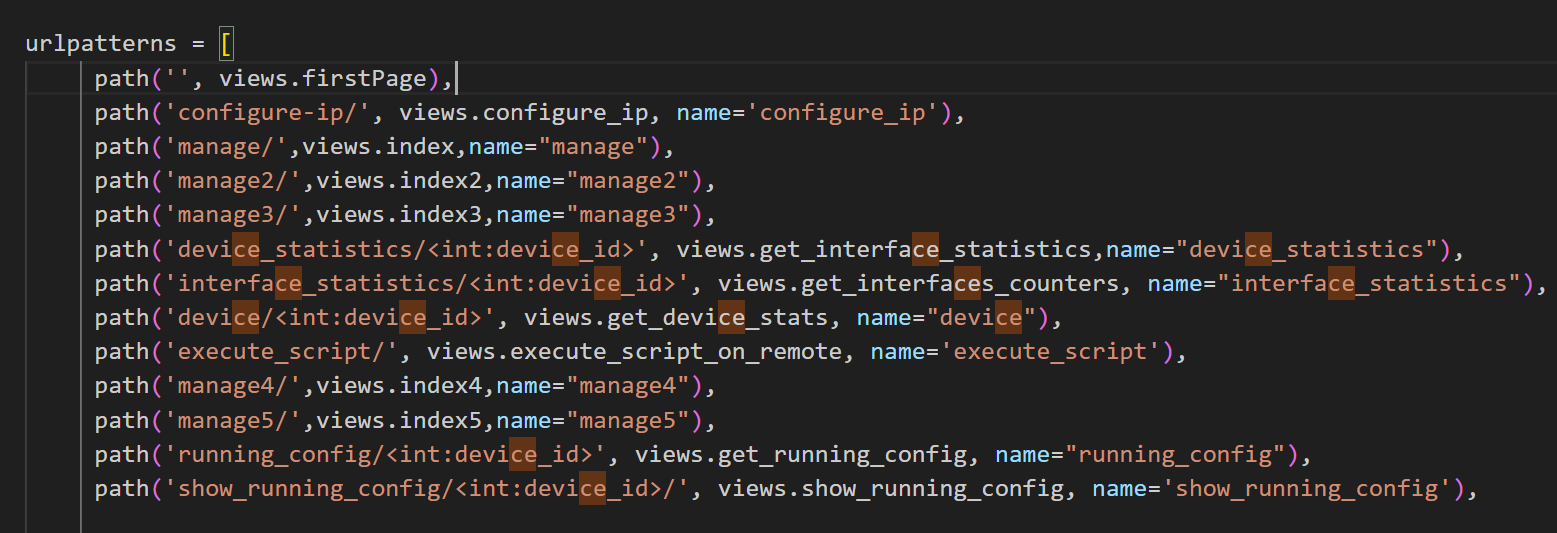
\includegraphics[width=1.0\textwidth]{graphics/urls.png}
	\caption{ \en{Urls.py} αρχείο}
\end{figure}

\FloatBarrier



\section{Η αρχική σελίδα της εφαρμοφής}

Προκειμένου να τρέξει ο \en{Django server}
τρέχουμε την εντολή η οποία βρίσκεται στην 
εικόνα 5.1.

\begin{figure}[h]
	\centering
	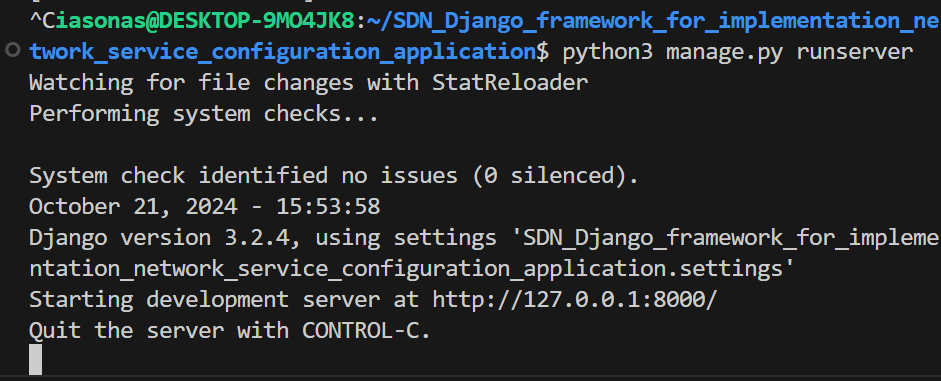
\includegraphics[width=1.0\textwidth]{graphics/django_server_run.png}
	\caption{ \en{Django run server}}
\end{figure}






Ο εξυπηρετητής τρέχει σαν διεργασία στο λειτουργικό
και είναι διαθέσιμος στη διεύθυνση \en{http://127.0.0.1:8000/}

Εάν εισάγουμε αυτή τη διεύθυνση σε έναν 
φυλλομετρητή της επιλογής μας, θα ανακατευθυνθούμε 
στην αρχική σελίδα, η οποία θα παρουσιαστεί στον 
χρήστη όπως στην εικόνα 5.2. Το εμπρόστιο τμήμα της εφαρμοφής(\en{frontend}) 
είναι γραμμένο με \en{HTML},\en{CSS} ενώ το οπίσθιο τμήμα(\en{backend}) 
είναι γραμμένο σε \en{Python}.

\begin{figure}[h]
	\centering
	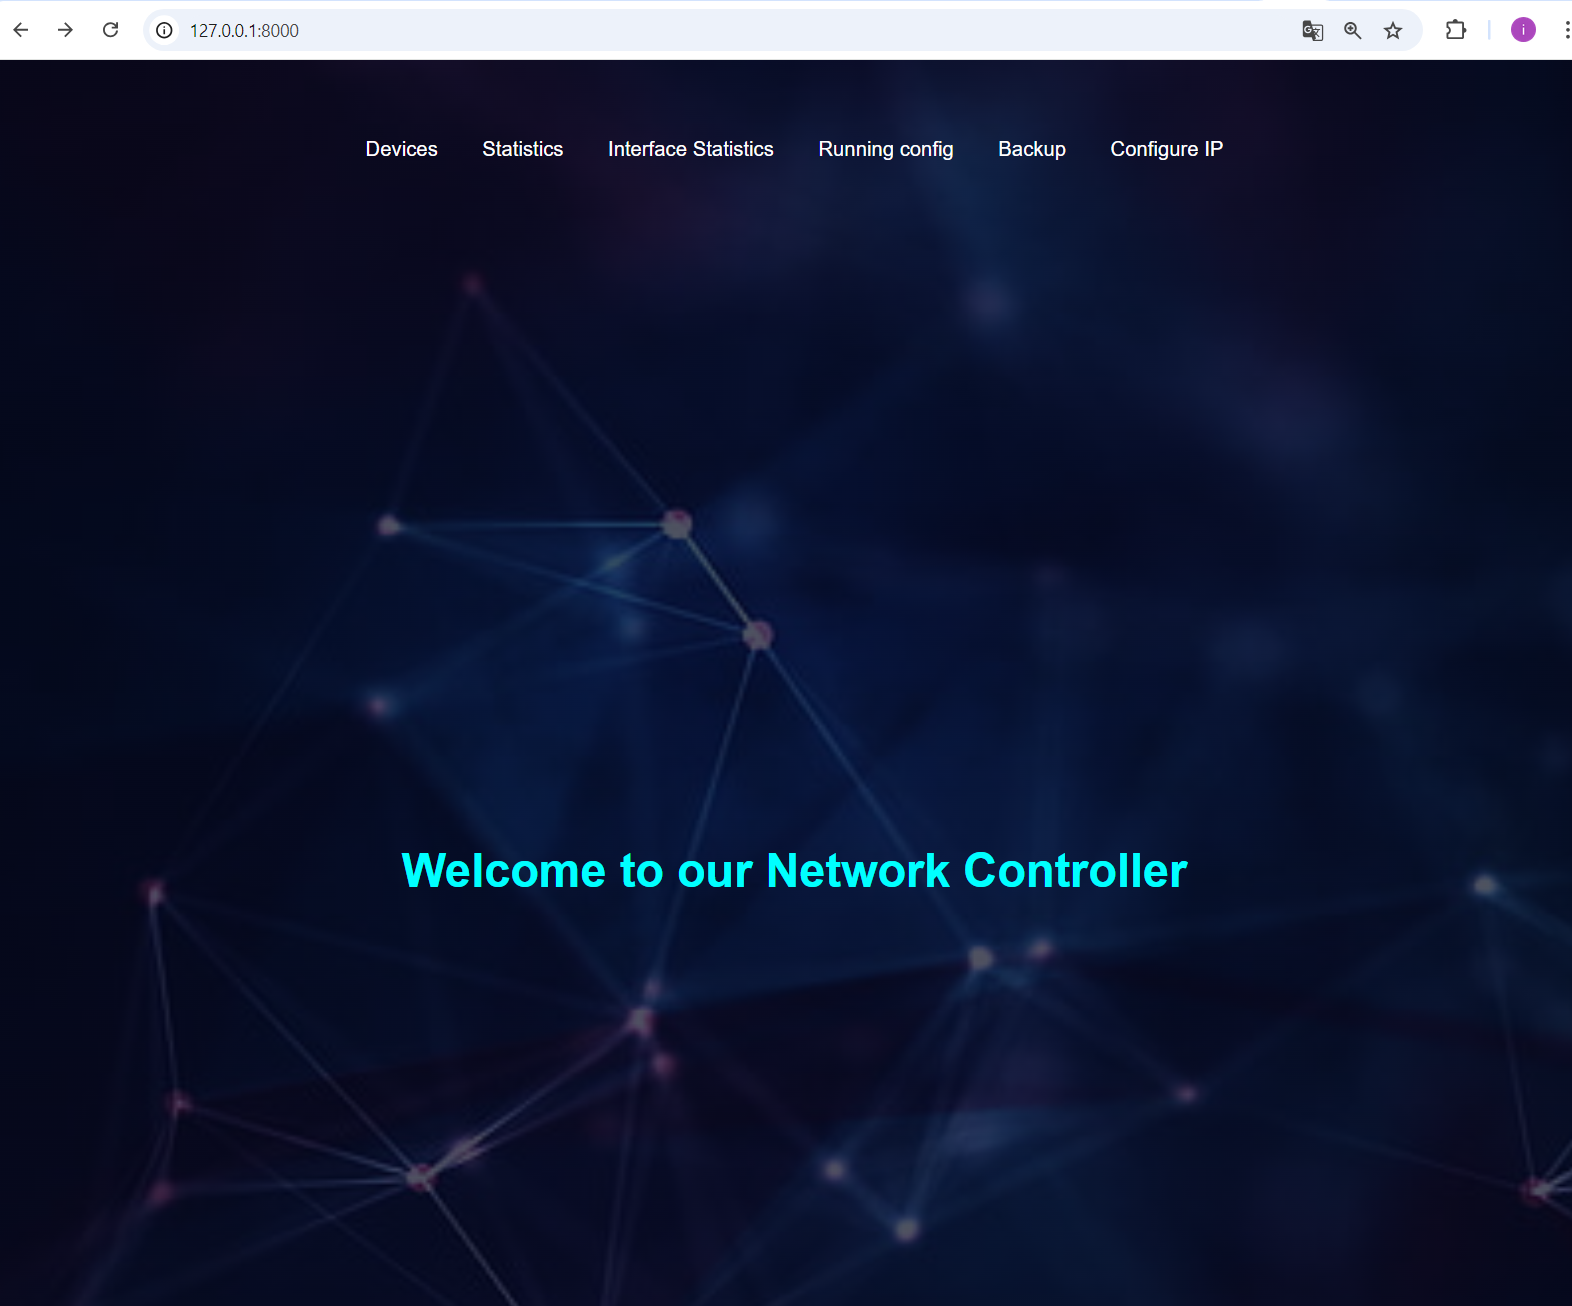
\includegraphics[width=1.2\textwidth]{graphics/home_page.png}
	\caption{ Αρχική Σελίδα}
\end{figure}

\FloatBarrier % Prevents floats from moving past this point

\section{\en{Devices}}

Προκειμένου να δημιουργήσουμε μία νεα συσκευή η παρακατω κλάσση
κώδικα μας βοηθάει στο να γίνει όπως στο σχήμα 5.3

\begin{figure}[htb]
	\centering
	\includegraphics[width=1.2\textwidth]{graphics/class_device.png}
	\caption{Αρχικοποίηση συσκευής}
\end{figure}

\FloatBarrier

Αφού λοιπόν πατήσουμε το κουμπί \en{Devices} αυτό θα μας δρομολογήσει στο αντίστοιχο \en{HTML link}.
Το οποίο θα μας εμφανίσει μια άλλη σελίδα αυτή του σχήματος 5.4. 

Αποτέλεσμα του πίνακα του σχήματος 5.4 είναι όλες οι συσκευές οι οποίες
είναι στη βάση δεδομένων μας όπου ο χρήστης πρόσθεσε προκειμένου
να μπορεί να αναδράσει με αυτές.

\begin{figure}[htb]
	\centering
	\includegraphics[width=1.2\textwidth]{graphics/device_interfaces.png}
	\caption{\en{Controller-Device Interfaces}}
\end{figure}

\FloatBarrier

Πατόντας ένα από αυτά τα κουμπιά θα μπορέσουμε να πάρουμε το αποτέλεσμα που θέλουμε.
Σε αυτή τη σελίδα μπορούμε να δούμε αν κάποια διεπαφή αν λειτουργεί ή όχι.
(Σχήμα 5.5)

\begin{figure}[htb]
	\centering
	\includegraphics[width=1.2\textwidth]{graphics/interfaces.png}
	\caption{\en{Interfaces}}
\end{figure}



\section{Στατιστικά της συσκευής}

Η λειτουργία του κουμπιού αυτού βασίζεται στη συνάρτηση \en{get\_interface\_statistics}, 
η οποία είναι υπεύθυνη για τη σύνδεση σε μια δικτυακή συσκευή, 
την απόκτηση στατιστικών πληροφοριών σχετικά με τις 
διεπαφές της, και την παρουσίαση αυτών των πληροφοριών 
σε μια ιστοσελίδα μέσω ενός προτύπου \en{HTML}. Η συνάρτηση αυτή 
δέχεται δύο παραμέτρους: το αίτημα του χρήστη (\en{request}) 
και το αναγνωριστικό της συσκευής (\en{device\_id}), 
το οποίο χρησιμοποιείται για να εντοπίσει τη συγκεκριμένη 
συσκευή από τη βάση δεδομένων.

Για να εντοπίσει τη συσκευή, παρουσιάζεται μία λίστα από το 
\en{User Interface} όπως και στην παραπάνω (\en{Devices}), 
και πατώντας πάνω της εμφανίζει τα παρακάτω στατιστικά:

\FloatBarrier

\begin{figure}[h]
	\centering
	\includegraphics[width=1.0\textwidth]{graphics/statistics.png}
	\caption{Στατιστικά}
\end{figure}

\section{Στατιστικά της διεπαφής}

Η συνάρτηση επιτρέπει τη σύνδεση σε μια δικτυακή συσκευή, την ανάκτηση των στατιστικών των διεπαφών της και την παρουσίαση αυτών των δεδομένων σε μια ιστοσελίδα

\FloatBarrier

\begin{figure}[h]
	\centering
	\includegraphics[width=1.0\textwidth]{graphics/interface_statistics.png}
	\caption{Στατιστικά διεπαφής}
\end{figure}


\section{\en{Backup} της συσκευής}

Προκειμένου να σώσουμε τη διαμόρφωση της συσκευής πατάμε το κουμπί
\en{backup} και με αυτό πέρνουμε το παρακάτω αποτέλεσμα.

Ουσιαστικά είναι σε \en{text} αρχείο το λεγόμενο \en{running config}
της συσκευής

\FloatBarrier

\begin{figure}[h]
	\centering
	\includegraphics[width=1.0\textwidth]{graphics/running_config.png}
	\caption{Τρέχων Διαμόρφωση}
\end{figure}


\section{Διαμόρφωση διεύθυνσης \en{IP}}

Η διαμόρφωση \en{IP} διεύθυσης γίνεται δίνοντας τα παρακάτω στοιχεία
σαν είσοδο

\FloatBarrier

\begin{figure}[h]
	\centering
	\includegraphics[width=1.0\textwidth]{graphics/configure_ip.png}
	\caption{\en{IP}Διαμόρφωση}
\end{figure}

Και καταφέρνει και αλλάζει την διέυθυνση.

\FloatBarrier

\begin{figure}[h]
	\centering
	\includegraphics[width=1.0\textwidth]{graphics/configure_ip_1.png}
	\caption{\en{IP} Διαφορά}
\end{figure}
\chapter{\en{Containerization} και \en{Deployment} }

\section{\en{Containerization} με \en{Docker}}

\subsection{Δημιουργία \en{Docker Image}}

Προκειμένου να μπορέσουμε να χρησιμοποιήσουμε το \en{Docker Desktop}, θα πρέπει να έχουμε δημιουργήσει την εφαρμογή μας σε μορφή \en{container}. Για να το πετύχουμε αυτό, είναι απαραίτητο να δημιουργήσουμε το \en{Dockerfile}(Σχήμα 8.1), το οποίο ουσιαστικά μετατρέπει την εφαρμογή μας σε \en{container}.
Προτού εξηγήσουμε τη διαδικασία δημιουργίας του \en{Image}, είναι σημαντικό να αναφέρουμε τον λόγο για τον οποίο πραγματοποιείται αυτή η διαδικασία. Οι \en{Cloud Native microservices} είναι σχεδιασμένες να λειτουργούν πάνω στην υποδομή του \en{Kubernetes}. Για να μπορέσει το \en{Kubernetes} να τις διαχειριστεί, πρέπει να γίνουν \en{deploy} σε αυτόν.
Ο \en{Kubernetes} δεν αναγνωρίζει εφαρμογές, ούτε \en{containers}, ούτε \en{Images} αλλά μόνο \en{pods}. Τα \en{pods} περιέχουν τα \en{containers}, τα οποία ουσιαστικά αποτελούν το λογισμικό που δημιουργείται μέσω της διαδικασίας δημιουργίας του \en{Image}. Ο Κυβερνήτης δεν αναγνωρίζει τίποτα άλλο εκτός από τα \en{pods}. Επειδή, λοιπόν, ο \en{Kubernetes} αναγνωρίζει \en{pods} που ορίζονται μέσω αρχείων \en{YAML}, τα οποία αναλύονται εκτενέστερα στην παράγραφο 8.2.1, δημιουργούμε το \en{Image} με τέτοιο τρόπο ώστε να μπορεί να το αναγνωρίσει ο \en{Kubernetes} στο τοπικό \en{Docker repository} και να προχωρήσει στη δημιουργία του \en{pod}.


\begin{figure}[htb]
	\centering
	\includegraphics[width=1.0\textwidth]{graphics/dockerfile.png}
	\caption{\en{Dockerfile}}
\end{figure}

\FloatBarrier


Tο \en{Dockerfile} του σχήματος 8.1 δηµιουργεί ένα περιβάλλον \en{Python 3.9} για ένα έργο \en{Django}. Ορίζει το φάκελο εργασίας στον κατάλογο \en{/app}, εγκαθιστά τις απαιτούµενες εξαρτήσεις από το αρχείο \en{requirements.txt}(σχήμα 8.4) , ενηµερώνει το \en{pip}, και εγκαθιστά βιβλιοθήκες συστήµατος (π.χ. \en{libyaml-dev}). Αντιγράφει τον κώδικα του έργου \en{Django} στο κοντέινερ, θέτει τη µεταβλητή περιβάλλοντος \en{PYTHONPATH}, εκθέτει την θύρα 8000 για τον διακοµιστή \en{Django} και εκκινεί την εφαρµογή µε την εντολή \en{runserver}.


Η εντολή \en{docker build}(σχήμα 8.2) χρησιμοποιείται για τη δημιουργία μιας εικόνας \en{Docker} (\en{Docker image}) 
από ένα συγκεκριμένο αρχείο \en{Dockerfile} και τα αρχεία που περιλαμβάνονται στον φάκελο εργασίας (\en{context}).

Αυτή η διαδικασία πακετάρει τον κώδικα της εφαρμογής, τις εξαρτήσεις και τις ρυθμίσεις σε ένα απομονωμένο περιβάλλον. 
Με αυτόν τον τρόπο, η παραγόμενη εικόνα μπορεί να διαμοιραστεί και να εκτελεστεί με συνέπεια σε διαφορετικά συστήματα, 
εξασφαλίζοντας ομοιόμορφο περιβάλλον εκτέλεσης. Είναι σημαντικό εργαλείο για αυτοματοποίηση και ανάπτυξη σε συστήματα \en{CI/CD}. Για να φτιάξουμε το \en{image} τρέχουμε τη εντολη \en{docker build -t djangothesis:v2}(σχήμα 8.2). Για να μπορέσουμε να τρέξουμε την εντολή αυτή πρέπει να βρισκόμαστε στο \en{path} που βρίσκεται το \en{requirements.txt} και το \en{manage.py}. Η διαδρομή φαίνεται στο σχήμα 8.3 και είναι ουσιαστικά εκεί που βρίσκεται και το \en{manage.py} αρχείο. 

\FloatBarrier

\begin{figure}[h]
	\centering
	\includegraphics[width=1.0\textwidth]{graphics/docker_build_v2.png}
	\caption{\en{Docker build}-Δημιουργία του κοντεινερ}
\end{figure}

\FloatBarrier


\FloatBarrier

\begin{figure}[h]
	\centering
	\includegraphics[width=1.0\textwidth]{graphics/dockerfile_location.png}
	\caption{\en{Dockerfile Path}}
\end{figure}

\FloatBarrier

\FloatBarrier

\begin{figure}[h]
	\centering
	\includegraphics[width=1.0\textwidth]{graphics/requirements.png}
	\caption{Αρχείο \en{requirements.txt}}
\end{figure}

\FloatBarrier

\noindent Τώρα που έγινε \en{build} το \en{image} είναι διαθέσιμο τοπικά(σχήμα 8.5) με το όνομα \en{djangothesis} και \en{tag v2} όπως αυτό ορίστηκε από την εντολή \en{docker build}(σχήμα 8.2).

\FloatBarrier


\begin{figure}[h]
	\centering
	\includegraphics[width=1.0\textwidth]{graphics/docker_image_list_2.png}
	\caption{\en{Docker image list}}
\end{figure}

\FloatBarrier



\section{\en{Deployment} με \en{Kubernetes}}

Τα τελευταία χρόνια, παρατηρείται ραγδαία αύξηση στον τομέα της πληροφορικής, 
με την εμφάνιση και εξάπλωση νέων εννοιών, όπως ο κυβερνήτης και τα \en{microservices}. 
Ένας βασικός παράγοντας που συνέβαλε στην εισαγωγή αυτών των τεχνολογιών είναι η ικανότητα εικονικοποίησης 
του λειτουργικού συστήματος, καθώς και η δυνατότητα εκτέλεσης εφαρμογών ως κοντέινερ. 
Αυτές οι τεχνολογίες επιτρέπουν την απομόνωση και τη διαχείριση εφαρμογών με μεγαλύτερη ευελιξία και 
αποτελεσματικότητα, κάτι που έχει οδηγήσει σε σημαντικές αλλαγές στον τρόπο ανάπτυξης και λειτουργίας των σύγχρονων υποδομών λογισμικού.

Τα κοντέινερ είναι ένας καλός τρόπος για να ομαδοποιήσουμε και να εκτελέσουμε τις εφαρμογές μας. 
Σε ένα περιβάλλον παραγωγής, πρέπει να διαχειριστούμε τα κοντέινερ που εκτελούν τις εφαρμογές και να 
διασφαλίσουμε ότι δεν υπάρχει χρόνος διακοπής λειτουργίας. Για παράδειγμα, εάν ένα κοντέινερ πέσει κάτω, ένα άλλο κοντέινερ πρέπει να ξεκινήσει. 

Το \en{Kubernetes} παρέχει ένα πλαίσιο για την εκτέλεση κατανεμημένων συστημάτων με μεγάλη ευχέρεια. Αναλαμβάνει τη διαχείριση της κλιμάκωσης και της ανθεκτικότητας (\en{failover}) μίας εφαρμογής, προσφέροντας παράλληλα διάφορα αναπτυξιακά μοτίβα και άλλες χρήσιμες δυνατότητες. Δεν είναι στόχος να αναλυθεί με κάθε λεπτομέρεια η λειτουργία του κυβερνήτη, καθώς κάτι τέτοιο απαιτεί μια ολόκληρη διπλωματική εργασία, αλλά θα παρουσιαστούν τα βασικά χαρακτηριστικά του που χρησιμοποιήθηκαν στην πράξη για την υλοποίηση της διπλωματικής εργασίας.



Στη διπλωματική αυτή εργασία, χρησιμοποιείται ένα τοπικό περιβάλλον 
ανάπτυξης με \en{Kubernetes} μέσω του \en{Minikube} και του \en{WSL2}
(\en{Windows Subsystem for Linux} 2) για την ανάπτυξη και δοκιμή 
της εφαρμογής \en{Django}. 

Το \en{Kubernetes} είναι μια δημοφιλής 
πλατφόρμα ενορχήστρωσης κοντέινερ, που επιτρέπει την αυτόματη 
διαχείριση και κλιμάκωση εφαρμογών σε περιβάλλοντα παραγωγής, 
ενώ το \en{Minikube} προσφέρει τη δυνατότητα εκκίνησης ενός 
τοπικού \en{Kubernetes cluster}. 
Με τον τρόπο αυτό, επιτυγχάνεται η δημιουργία ενός ασφαλούς, 
απομονωμένου περιβάλλοντος δοκιμών, το οποίο προσομοιώνει ένα 
πλήρες \en{cluster}, χωρίς την ανάγκη πρόσθετης υποδομής \en{cloud}.

Χάρη στο \en{WSL2}, το οποίο επιτρέπει την εκτέλεση \en{Linux} 
πυρήνα απευθείας στα \en{Windows}, 
εξασφαλίζεται ευκολία στη διαχείριση του \en{cluster} 
και της εφαρμογής \en{Django}, 
ενώ η χρήση εργαλείων όπως το \en{kubectl} 
καθιστά εύκολη την παρακολούθηση και τον έλεγχο των \en{pods} 
και υπηρεσιών. Αυτό το περιβάλλον προσφέρει μια ολοκληρωμένη 
εμπειρία ανάπτυξης και δοκιμής, βοηθώντας στην κατανόηση των 
αρχών του \en{Kubernetes} και διευκολύνοντας τη μετάβαση της 
εφαρμογής σε μεγαλύτερα \en{production} περιβάλλοντα

Το \en{Minikube} είναι ένα εργαλείο που απλοποιεί την εκτέλεση και 
διαχείριση ενός τοπικού \en{Kubernetes cluster} στον υπολογιστή σας,
ειδικά σχεδιασμένο για περιβάλλοντα ανάπτυξης και δοκιμών. 
Σας επιτρέπει να ξεκινήσετε ένα \en{Kubernetes cluster} 
με ένα μόνο κόμβο (ή ακόμα και πολλούς σε ορισμένες περιπτώσεις) 
χρησιμοποιώντας εικονικοποίηση μέσω \en{WSL, Docker, ή Hypervisor}. 
Ο κύριος σκοπός του \en{Minikube} είναι να παρέχει ένα περιβάλλον \en{Kubernetes} 
με όλες τις βασικές δυνατότητες του \en{Kubernetes} 
αλλά χωρίς την πολυπλοκότητα που θα απαιτούσε η διαχείριση ενός \en{cluster}
σε παραγωγικό περιβάλλον.

Επιπλέον, το \en{Minikube} 
διαθέτει ενσωματωμένα εργαλεία, όπως τη δυνατότητα να παρακολουθείτε
και να διαχειρίζεστε τον πίνακα ελέγχου του \en{Kubernetes}, 
να δημιουργείτε \en{pods, deployments}, και \en{services}[19], και 
να παρακολουθείτε τα \en{logs} των εφαρμογών σας, ενώ επιτρέπει 
επίσης εύκολη σύνδεση με εργαλεία όπως το \en{kubectl} 
για πλήρη πρόσβαση στη διαχείριση του \en{cluster}. 
Αυτό το καθιστά ιδανικό για προγραμματιστές που θέλουν να 
πειραματιστούν με \en{Kubernetes}, 
να κάνουν δοκιμές εφαρμογών, ή να αναπτύξουν μικροϋπηρεσίες 
τοπικά χωρίς να απαιτείται η πολυπλοκότητα ενός πλήρους \en{cluster}
όπως το περιβάλλον της παρούσας διπλωματικής εργασίας. Παρακάτω μπορούμε να δούμε 
πόσο εύκολα μπορούμε να ξεκινήσουμε ένα τοπικό περιβάλλον κυβερνήτη(σχήμα 8.5).


\begin{figure}[h]
	\centering
	\includegraphics[width=1.0\textwidth]{graphics/minikube_deployment_k8s.png}
	\caption{\en{Minikube deployment}}
\end{figure}

\subsection{Δημιουργία \en{Kubernetes manifest files}}

Στο πλαίσιο της ανάπτυξης της εφαρμογής, χρησιμοποιήθηκε το 
\en{Kubernetes} για τη δημιουργία και διαχείριση ενός \en{pod} 
που φιλοξενεί την εφαρμογή \en{Django}. Το αρχείο διαμόρφωσης \en{YAML}
(\en{pod1.yml}) που δημιουργήθηκε, ακολουθεί τη βασική δομή του \en{Kubernetes}, 
ορίζοντας τον τύπο πόρου ως \en{Pod} και 
εκχωρώντας μεταδεδομένα όπως το όνομα \en{djangotestapp}. 
Στην ενότητα \en{spec}, ορίζεται ένα \en{container} 
το οποίο χρησιμοποιεί την εικόνα \en{iasonasi/djangotestapp:latest} 
και ακούει στη θύρα 8000, η οποία είναι η προεπιλεγμένη θύρα της 
εφαρμογής \en{Django}. Παρακάτω το \en{spec} του \en{yaml file.}(σχήμα 8.7)

\FloatBarrier

\begin{figure}[h]
	\centering
	\includegraphics[width=1.0\textwidth]{graphics/pod_spec.png}
	\caption{\en{Spec} του \en{YAML file}}
\end{figure}

\FloatBarrier

Αυτό το παράδειγμα αποδεικνύει τη σημασία της χρήσης του \en{Kubernetes YAML syntax} 
για την αυτοματοποιημένη ανάπτυξη και διαχείριση \en{containerized} 
εφαρμογών. Μέσω αυτής της διαδικασίας, η εφαρμογή μπορεί να 
επεκταθεί εύκολα σε διάφορα περιβάλλοντα και να κλιμακωθεί 
ανάλογα με τις ανάγκες. Το συγκεκριμένο αρχείο \en{YAML} 
επιτρέπει στο \en{Kubernetes} να εκτελέσει και να διαχειριστεί το 
\en{pod} με τρόπο ανεξάρτητο από το υποκείμενο σύστημα, 
εξασφαλίζοντας επαναληψιμότητα και δυνατότητα μεταφοράς του 
συστήματος σε διαφορετικές υποδομές. Στην παρακάτω εικόνα φαίνεται το 
\en{YAML file} που χρησιμοποιήθηκε(σχήμα 8.8). 

\FloatBarrier

\begin{figure}[h]
	\centering
	\includegraphics[width=1.0\textwidth]{graphics/deploy_django.png}
	\caption{\en{Manifest for Django pod}}
\end{figure}

\FloatBarrier

\subsection{Πρόσβαση στο \en{Django pod}}.

Για να αποκτήσουμε πρόσβαση στην εφαρμογή \en{Django} που τρέχει στο \en{pod} του \en{Kubernetes}, 
μπορούμε να χρησιμοποιήσουμε την εντολή \en{kubectl port-forward pod/djangotestapp 8000:8000}. Με την εντολή \en{kubectl port-forward} θα μπορέσουμε μέσα απο έναν \en{browser}
να έχουμε πρόσβαση στην εφαρμογή.

\FloatBarrier

\begin{figure}[h]
	\centering
	\includegraphics[width=1.0\textwidth]{graphics/kubernetes_proxy.png}
	\caption{Πρόσβαση στο \en{Django pod} μέσα από τη λειτουργία \en{Port forward}}
\end{figure}

\FloatBarrier

\noindent  Στη συνέχεια, η εφαρμογή είναι προσπελάσιμη στην διεύθυνση \en{http://localhost:8000}. Όλες οι λειτουργίες θα πρέπει να μπορούν να εκτελεστούν, όπως και επιβεβαιώνεται από την εικόνα στο σχήμα 8.9.

\section{\en{Use cases} με \en{Kubernetes}}

Η ανάπτυξη μιας εφαρμογής σε περιβάλλον \en{Kubernetes} στοχεύει στη μετατροπή της σε μικροϋπηρεσία, προσφέροντας σημαντικά πλεονεκτήματα. Αυτή η αρχιτεκτονική διευκολύνει την κλιμάκωση μέσω των μηχανισμών του \en{Kubernetes}, όπως το \en{Horizontal Pod Autoscaler} (\en{HPA}), το οποίο επιτρέπει την αυτόματη προσαρμογή των πόρων της εφαρμογής προσθέτοντας επιπλέον \en{replica}. Στο πλαίσιο της παρούσας διπλωματικής εργασίας, η υλοποίηση περιορίστηκε στη δημιουργία \en{pod}. Παρόλα αυτά, η μετατροπή της εφαρμογής σε μικροϋπηρεσία διευκολύνει την αξιοποίηση των δυνατοτήτων του \en{Kubernetes}, καθώς η ενσωμάτωση οποιουδήποτε αντικειμένου, όπως το \en{HPA}, πραγματοποιείται εύκολα μέσω της κατάλληλης διαμόρφωσης σε \en{YAML file}.

Η χρήση \en{Kubernetes} στη συγκεκριμένη εφαρμογή αποσκοπεί στην αύξηση της ευελιξίας και της προσαρμοστικότητάς της σε περιόδους υψηλής ζήτησης. Ενώ μια μονολιθική εφαρμογή παρουσιάζει περιορισμούς στην επέκταση, η αρχιτεκτονική μικροϋπηρεσιών επιτρέπει δυναμική κλιμάκωση, διασφαλίζοντας τη βέλτιστη λειτουργία της εφαρμογής σε κάθε συνθήκη.

Το παρόν αρχείο \en{YAML} της εικόνα 8.10 περιγράφει έναν πόρο τύπου \en{Deployment} στο \en{Kubernetes}, με σκοπό την αυτόματη ανάπτυξη και διαχείριση μιας \en{web} εφαρμογής \en{Django}. Ο πόρος αυτός ονομάζεται \en{django-app} και χρησιμοποιεί το \en{label app}: \en{django} για τη σήμανση τόσο του ίδιου όσο και των \en{pods} που θα δημιουργήσει, διευκολύνοντας έτσι τη σύνδεσή του με άλλα αντικείμενα του \en{Kubernetes}, όπως \en{Services} ή \en{selectors}. 

Ορίζεται η δημιουργία δύο αντιγράφων (\en{replicas}) της εφαρμογής, ώστε να διασφαλίζεται η διαθεσιμότητα και η αντοχή σε αστοχίες. Κάθε \en{pod} περιέχει έναν \en{container}, ο οποίος βασίζεται στην εικόνα \en{Docker iasonasi/djangotestapp:latest}. Η εικόνα αυτή προφανώς περιλαμβάνει την \en{Django} εφαρμογή. O \en{container} εκθέτει την πόρτα 8000, η οποία χρησιμοποιείται συνήθως για \en{web} εφαρμογές \en{Django}.

Συνολικά, το \en{Deployment} αυτός διασφαλίζει ότι η εφαρμογή \en{Django} θα τρέχει με συνέπεια και αξιοπιστία, καθώς το \en{Kubernetes} θα φροντίζει να υπάρχουν πάντα δύο ενεργά \en{pods}. Αν κάποιο \en{pod} αποτύχει, το σύστημα θα το αντικαταστήσει αυτόματα. Στη διπλωματική αυτή δε χρησιμοποιήσαμε \en{Services} αλλά μπορέσαμε να κάνουμε την εφαρμογή προσβάσιμη μέσα από την εντολή \en{kubectl port-forward} όπως φαίνεται και στο σχήμα 8.9.

\FloatBarrier

\begin{figure}[h]
	\centering
	\includegraphics[width=1.0\textwidth]{graphics/kubernetes_use_case.png}
	\caption{\en{Deployment yaml for Django pod} }
\end{figure}

\chapter{Συμπέρασματα και Μελλοντική Εργασία}

\section{Συμπεράσματα}

Η διπλωματική αυτή εργασία επικεντρώθηκε στην ανάπτυξη ενός εργαλείου αυτοματοποίησης 
δικτύου με χρήση της γλώσσας προγραμματισμού \en{Python}. 
Κατά τη διάρκεια αυτής της διαδικασίας, καταφέραμε να αναπτύξουμε και να 
εφαρμόσουμε διάφορες τεχνολογίες για την αυτοματοποίηση δικτυακών εργασιών, 
όπως η διαμόρφωση συσκευών και η παρακολούθηση της απόδοσης του δικτύου. 
Το εργαλείο αναπτύχθηκε χρησιμοποιώντας σαν \en{TestBed} το \en{GNS3} και το \en{Cisco IOU}, 
και παρέχει σημαντικά οφέλη στον τομέα της δικτύωσης.




\section{Προκλήσεις και Μαθήματα}


Οι προκλήσεις που αντιμετωπίστηκαν κατά τη διάρκεια της 
εργασίας περιελάμβαναν τη διαχείριση περιορισμών, όπως η 
εύρεση της κατάλληλης έκδοσης \en{Cisco IOU}, μια διαδικασία 
χρονοβόρα λόγω της μη δημόσιας διαθεσιμότητάς τους. 
Αυτό απαίτησε χρόνο για έρευνα και επίλυση τεχνικών προβλημάτων, 
οδηγώντας σε καθυστερήσεις, αλλά και σε πολύτιμα μαθήματα για τη 
διαχείριση κρίσιμων πόρων και την επιμονή στις δυσκολίες. Η εκμάθηση 
της \en{Python} υπήρξε εξίσου απαιτητική, καθώς απαιτούσε 
εμβάθυνση στη σύνταξη, στις δομές δεδομένων και στον προγραμματισμό. 
Οι δυσκολίες αυτές έγιναν ευκαιρίες κατανόησης της δύναμης της 
γλώσσας, ειδικά στον τομέα της αυτοματοποίησης. Η εμπειρία αυτή 
ανέδειξε τη σημασία της κριτικής σκέψης και της δημιουργίας 
ρεαλιστικών λύσεων.

Τέλος, η ανάπτυξη της εφαρμογής έδειξε πώς οι 
τεχνικές προκλήσεις μπορούν να μετατραπούν σε μαθήματα ζωής, 
όπως η διαχείριση χρόνου, η συνεργασία με εργαλεία ανοιχτού 
κώδικα και η ανάγκη για συνεχή ενημέρωση σε νέες τεχνολογίες. 
Η εργασία ανέδειξε τη σημασία της προσαρμοστικότητας και της 
δια βίου μάθησης στον τομέα των δικτύων

\section{Μελλοντική Εργασία και Επέκταση Λειτουργικότητας}

Η μελλοντική εργασία θα επικεντρωθεί στην περαιτέρω 
βελτίωση της λειτουργικότητας της εφαρμογής, ενσωματώνοντας 
επιπλέον πρωτόκολλα δικτύωσης και αυτοματοποίησης. 
Μια πιθανή κατεύθυνση είναι η ανάπτυξη μηχανισμών για την 
υποστήριξη \en{SDN} (δικτύωση οριζόμενη από λογισμικό), 
προκειμένου να ανταποκριθεί στις απαιτήσεις σύγχρονων δικτύων.

Επίσης, θα μπορούσαν να προστεθούν χαρακτηριστικά όπως 
η παρακολούθηση της απόδοσης του δικτύου σε πραγματικό 
χρόνο και η αυτοματοποίηση διαδικασιών αποκατάστασης προβλημάτων. 
Οι επεκτάσεις θα ενισχύσουν την ευελιξία και τη χρηστικότητα του 
εργαλείου.

Το περιβάλλον της εφαρμογής θα μπορούσε να είναι διαφορετικό.
Μελλοντική εργασία μπορεί να αναπτυχθεί με τη βοήθεια καινούργιων περιβάλλοντων προσομοιώσης όπως
το \en{ContainerLab}. Η περαιτέρω ανάπτυξη λειτουργιών της εφαρμογής, η δημιουργία καλυτερου \en{User Experience}
και \en{User Interface} καθώς και η δημιουργία \en{Testing Platform} για την αυτοματοποίηση
του \en{testing} της εφαρμογής θα μπορούσαν να αποτελέσουν ξεχωριστό επίσης θέμα για διπλωματική εργασία.

Τέλος, η μελλοντική έρευνα μπορεί να εξετάσει τη δυνατότητα διασύνδεσης με 
πλατφόρμες μηχανικής μάθησης, για την 
πρόβλεψη και αποτροπή πιθανών αποτυχιών, 
καθιστώντας την εφαρμογή ένα σύγχρονο εργαλείο 
αυτοματοποιημένης διαχείρισης δικτύου

\chapter{Παράρτημα}

\section{Σχεδίαση και Διάγραμμα τοπολογίας δικτύου}

\FloatBarrier

\begin{figure}[h]
	\centering
	\includegraphics[width=1.1\textwidth]{graphics/network_topology_high_level.png}
	\caption{\en{Network topology design}}
\end{figure}

\FloatBarrier

\section{Οδηγός χρήσης της εφαρμογής}

\subsection{Δημιουργία αντικειμένου-Προσθήκη συσκευής}

Προκειμένου να μπορούμε να διαχειριστούμε συσκευή θα πρέπει να την εισάγουμε ως αντικείμενο.

Ανοίγουμε το \en{http://127.0.0.1:8000/admin/} σε \en{browser} και εισάγουμε ως χρήστη \en{iasonas}
και κωδικό \en{ericsson}.

\FloatBarrier

\begin{figure}[h]
	\centering
	\includegraphics[width=1.1\textwidth]{graphics/GUI_LOGIN.png}
	\caption{\en{GUI Login}}
\end{figure}

\FloatBarrier

Αφού συνδεθούμε στο \en{GUI} επιλέγουμε \en{Network}, \en{Devices} και \en{Add} προκειμένου να εισάγουμε καινούργια συσκευή.

\FloatBarrier

\begin{figure}[h]
	\centering
	\includegraphics[width=1.1\textwidth]{graphics/DJANGO_ADMIN.png}
	\caption{\en{GUI Login second page}}
\end{figure}

\FloatBarrier

Στη συνέχεια μας εμφανίζεται η παρακάτω εικόνα. Βάζουμε τα στοιχεία της συσκευής και πατάμε αποθήκευση.

\FloatBarrier

\begin{figure}[h]
	\centering
	\includegraphics[width=1.1\textwidth]{graphics/ADD_DEVICE.png}
	\caption{\en{Add device page}}
\end{figure}

\FloatBarrier

Αφού το κάνουμε αυτό όλες οι συσκευές που προσθέσαμε μπορούμε να τις δούμε σε όλες τις λειτουργίες της εφαρμογής.
Οι λειτουργίες μπορούν να εκτελεστούν μια μια όπως έγινε στο \en{application demo}.

\section{Κώδικας}

H εφαρμογή είναι ελεύθερη στη σελίδα:


\FloatBarrier

\begin{figure}[h]
	\centering
	\includegraphics[width=1.1\textwidth]{graphics/github_page.png}
	\caption{\en{github repo}}
\end{figure}

\FloatBarrier


\chapter{Βιβλιογραφία}

%Το \en{Lorem Ipsum} είναι απλά ένα κείμενο χωρίς νόημα για τους επαγγελματίες της τυπογραφίας και στοιχειοθεσίας \cite{LoremIpsumAll}. Το \en{Lorem Ipsum} είναι το επαγγελματικό πρότυπο όσον αφορά το κείμενο χωρίς νόημα, από τον 15ο αιώνα, όταν ένας ανώνυμος τυπογράφος πήρε ένα δοκίμιο και ανακάτεψε τις λέξεις για να δημιουργήσει ένα δείγμα βιβλίου. Όχι μόνο επιβίωσε πέντε αιώνες, αλλά κυριάρχησε στην ηλεκτρονική στοιχειοθεσία, παραμένοντας με κάθε τρόπο αναλλοίωτο. Έγινε δημοφιλές τη δεκαετία του '60 με την έκδοση των δειγμάτων της \en{Letraset} όπου περιελάμβαναν αποσπάσματα του \en{Lorem Ipsum}, και πιο πρόσφατα με το λογισμικό ηλεκτρονικής σελιδοποίησης όπως το \en{Aldus PageMaker} που περιείχαν εκδοχές του \en{Lorem Ipsum}.

\section{Βιβλιογραφίκές αναφορές}
\begin{itemize}
    \item \en{https://kubernetes.io/docs/concepts/overview/}  
    \item \en{Vs Code development environment}
    \item \en{https://el.wikipedia.org/wiki/}
    \item \en{Virtual box} ή οποιονδήποτε \en{type B hypervisor}
    \item \en{https://www.cloudflare.com/learning/network-layer/what-is-the-control-plane/}
    \item \en{https://el.wikipedia.org/wiki/Git}
    \item \en{https://kubernetes.io}
    \item \en{https://github.com/dmfigol/network-programmability-stream}
    \item \en{https://medium.com/@komalminhas.96/a-step-by-step-guide-to-build-and-push-your-own-docker-images-to-dockerhub-709963d4a8bc}
    \item \en{https://repository.ihu.edu.gr/}, \en{Network automation using python George Milios}
    \item \en{Wikipedia}, τι είναι το \en{Windows Subsystem for Linux}
    \item \en{wikipedia.org/wiki/Modelviewcontroller}
\end{itemize}


%\begin{equation}
%	y = \alpha x + \beta
%\end{equation}

%Αντίθετα με αυτό που θεωρεί η πλειοψηφία, το \en{Lorem Ipsum} δεν είναι απλά ένα τυχαίο κείμενο. Οι ρίζες του βρίσκονται σε ένα κείμενο Λατινικής λογοτεχνίας του 45 π.Χ., φτάνοντας την ηλικία του πάνω από 2000 έτη.


%\begin{figure}[htb]
%	\centering
%	\includegraphics{tikz/hsv_cone/hsv_cone.pdf}
%	\caption{Ο χρωματικός χώρος \en{HSV}.}
%\end{figure}


\end{document}
